\documentclass[conference,a4paper,10pt]{IEEEtran}
%\documentclass{article}
\IEEEoverridecommandlockouts

% General
\usepackage[T1]{fontenc} % optional T1 font encoding
\usepackage[utf8]{inputenc}
\usepackage[english]{babel}
\usepackage{glossaries}
%A
\newacronym{AWGN}{AWGN}{additive white gaussian noise}
\newacronym{AF}{AF}{array factor}
%B
\newacronym{BS}{BS}{base station}

%C
\newacronym{CE}{CE}{channel estimation}
\newacronym{CDF}{CDF}{cumulative distribution function}
\newacronym{CP}{CP}{cyclic prefix}
\newacronym{CMS}{CMS}{canonical minimum-scattering}
\newacronym{CSI}{CSI}{channel state information}

%D+
\newacronym{DFT}{DFT}{discrete fourier transform}
\newacronym{DTFT}{DTFT}{discrete time fourier transform}
\newacronym{DMA}{DMA}{dynamic metasurface antenna}
\newacronym{DL}{DL}{downlink}

%E
\newacronym{ELAA}{ELAA}{extremely large aperture array}

%F
\newacronym{flop}{flop}{floating point operation}
\newacronym{flops}{flops}{\gls{flop} per second}
\newacronym{FD}{FD}{full-digital}
\newacronym{FDMA}{FDMA}{Frequency division multiple access}

%G

\newacronym{LOS}{LoS}{Line-of-Sight}

\newacronym{NLOS}{NLoS}{Non-Line-of-Sight}

\newacronym{ISAC}{ISAC}{integrated sensing and communication}

\newacronym{OMP}{OMP}{orthogonal matching pursuit}
\newacronym{OFDM}{OFDM}{orthogonal-frequency division multiplexing}

% M
\newacronym{MINLP}{MINLP}{mixed integer non-linear problem}

%R
\newacronym{RF}{RF}{radio-frequency}
\newacronym{RIS}{RIS}{reconfigurable intelligent surface}
\newacronym{RB}{RB}{resource block}

%S
\newacronym{SE}{SE}{spectral efficiency}
\newacronym{SINR}{SINR}{signal-to-interference-plus-noise ratio}
\newacronym{SNR}{SNR}{signal-to-noise ratio}
\newacronym{SLL}{SLL}{side lobe level}

%T
\newacronym{TDD}{TDD}{time division duplexing}
\newacronym{TDMA}{TDMA}{time division multiple access}

%U
\newacronym{UE}{UE}{user equipment}
\newacronym{UL}{UL}{uplink}
\newacronym{ULA}{ULA}{uniform linear array}

%V
\newacronym{VR}{VR}{visibility region}

%X

%Y

%Z

% Writing
\usepackage{lmodern}
\usepackage{comment}
\usepackage[colorlinks=true, allcolors=blue]{hyperref}
\usepackage{extarrows}
\usepackage{cite}
\usepackage[normalem]{ulem}
\hyphenation{op-tical net-works semi-conduc-tor}
% Plotting
\usepackage[svgnames]{xcolor}
\usepackage[pdftex]{graphicx}
\usepackage{caption}
\usepackage{subcaption}
% Tikz
\usepackage{tikz}
\usetikzlibrary{math, shapes}
\usepackage{pgfplots}
\pgfplotsset{
compat=1.3,
legend style={font=\scriptsize, fill opacity=0.8,  draw opacity=1, text opacity=1, draw=white!15!black, legend cell align=left, align=left}, 
width=6.5cm, 
yminorticks=false,
xminorticks=false,
title style={font=\small},
tick style={color=black},
tick label style={font=\small},
tick align=outside,
grid style={line width=.1pt, draw=gray!20},
major grid style={line width=.1pt,draw=gray!20},
label style={font=\small},
}
% Math
\usepackage{amssymb,amsmath,amsfonts,amsthm,bm,mathtools,cuted,bbold}
\usepackage[cmintegrals]{newtxmath}
\usepackage{cuted}
% Table
\usepackage{tabularx}
\usepackage{booktabs}
\usepackage[ruled,vlined,linesnumbered]{algorithm2e}

% New commands
\newcommand{\T}{^{\intercal}}     % transpose
\renewcommand{\H}{^{\rm {H}}}   % hermitian
\newcommand{\E}[1]{\mathbb{E}\left\{ #1 \right\}} % expectation
\newcommand{\mc}[1]{\mathcal{#1}}   % mathcal abbreviation
\newcommand{\mb}[1]{\mathbf{#1}}    % mathbold abbreviation
\newcommand{\dpar}[2]{\mathop{}\!\frac{\partial #1}{\partial #2}}   % partial derivative
\newcommand*\diff{\mathop{}\!\mathrm{d}}    % differential in the integral
\DeclareMathOperator*{\argmax}{arg\,max}    % argmax
\DeclareMathOperator*{\argmin}{arg\,min}    % argmin
\DeclareMathOperator{\sinc}{sinc}

\newcommand{\DL}{^{\rm \scriptscriptstyle {DL}}} 
\newcommand{\UL}{^{\rm \scriptscriptstyle {UL}}} 
\newcommand{\HPp}{^{\rm \scriptscriptstyle {HP+}}}
\newcommand{\HPm}{^{\rm \scriptscriptstyle {HP-}}}


% Comments
\definecolor{gold}{rgb}{0.85,.66,0}
\definecolor{amaranth}{rgb}{0.9, 0.17, 0.31}


% COMMENTS
\newcommand{\TODO}[1]{\textcolor{orange}{TODO: {#1}}} % TODO commenting
\newcommand{\colb}{\textcolor{blue}} % used to highlight general changes
\newcommand{\colr}{\textcolor{red}} % used for problems in general 
\newcommand{\pp}[1]{\textcolor{blue}{ {#1}}} % Petar
\newcommand{\fs}[1]{\textcolor{amaranth}{#1}} % Fabio variations
\newcommand{\FS}[1]{\textcolor{amaranth}{\footnotesize \textsf{[Fabio: #1]}}} % Fabio comments
\newcommand{\KK}[1]{\textcolor{blue}{\footnotesize \textsf{[Kimmo: #1]}}} % Kimmo comments

\newtheorem{assumption}{Assumption}
\newtheorem{lemma}{Lemma}

%\title{A RIS-aided OFDM communication protocol exploiting positioning information}
% \title{Position based resource allocation with RIS in frequency selective channels}
\title{Localization-based OFDM framework for RIS-aided systems}
%\title{Why RIS chennels are inheretely frequency selective and how to fix it.}
\author{\IEEEauthorblockN{Fabio Saggese\IEEEauthorrefmark{1}, Kimmo Kansanen\IEEEauthorrefmark{1}\IEEEauthorrefmark{2}, and Petar Popovski\IEEEauthorrefmark{1}}
\IEEEauthorblockA{\IEEEauthorrefmark{1}Department of Electronic Systems, Aalborg University, Denmark (\{fasa, kimkan, petarp\}@es.aau.dk)}
\IEEEauthorblockA{\IEEEauthorrefmark{2}Department of Electronic Systems, Norwegian University of Science and Technology}\thanks{This work was partly supported by the Villum Investigator grant ``WATER'' from the Villum Foundation, Denmark, and by the Horizon 2020 ``RISE-6G'' project, financed by the European Commission under grant no. 101017011.}}

\begin{document}

\maketitle

\begin{abstract}
Efficient integration of reconfigurable intelligent surfaces (RISs) into the current wireless network standard is not a trivial task due to the overhead generated by performing channel estimation (CE) and phase-shift optimization. In this paper, we propose a framework enabling the coexistence between orthogonal-frequency division multiplexing (OFDM)
and RIS technologies. Instead of wasting communication symbols for the CE and optimization, the proposed framework exploits the localization information obtainable by RIS-aided communications to provide a robust
allocation strategy for user multiplexing. The results demonstrate the effectiveness of the proposed approach with respect to CE-based transmission methods.
\end{abstract}
\begin{IEEEkeywords}
Reconfigurable intelligent surfaces, OFDM, robust optimization, resource allocation
\end{IEEEkeywords}


\section{Introduction}
\Glspl{RIS} are considered among the enabling technologies for the next-generation (6G) of wireless networks due to their ability to control the wireless propagation environment~\cite{bjornson2021signalprocessing}. 

In recent years, many research works have shown the capabilities of the \gls{RIS} in terms of improved coverage, data rate, and mitigation of multi-user interference through accurate phase-shift optimization~\cite{mengnan2022survey}. 
However, only a few works have focused on integrating the \gls{RIS} into the existing communication protocols. To the best of the authors' knowledge, the authors of~\cite{Zheng2020cebf} were the first to consider \gls{RIS}-aided communications framework employing \gls{OFDM}, proposing a joint \gls{CE} and \gls{RIS} phase-shift optimization framework showing outstanding performance for a single \gls{UE} scenario.
Nevertheless, in multi-user systems, \gls{RIS} channel estimation procedures need pilot sequences whose length is proportional to the number of \gls{RIS} elements and the number of \glspl{UE} in the system~\cite{Wang2020ce, mengnan2022survey}. Hence, the \gls{CE} procedure may lead to an unfeasible overhead when serving a large number of users.
% \fs{While the effort of the community in reducing this overhead, it is still unclear if the \gls{RIS} can be integrated to the \gls{OFDM} classically.}

From a different perspective, the recent literature has shown the capability of using \gls{RIS} to enhance the performance of localization algorithms~\cite{bjornson2021signalprocessing}, and even enable new localization procedures not feasible without an \gls{RIS}~\cite{keykhosravi2021siso}.
Considering the relevance that \gls{ISAC} has gained to enable the \emph{connected intelligence} promised by the 6G, it is natural to imagine the use of the (improved) localization information available in \gls{RIS}-aided networks to help the scheduling decision: instead of wasting time for exchanging \gls{CE} pilot sequences, the knowledge of the \glspl{UE} position can be used to optimize the data transmission.
In this line, the authors of~\cite{Abrardo2021positioning} proposed a \gls{RIS} phase shift optimization based on localization information able to maximize the average spectral efficiency. Furthermore, in~\cite{wang2021joint}, the authors provide a \gls{TDD} framework to integrate communication and localization in \gls{RIS}-aided systems.

This paper proposes an \gls{OFDM} scheduling protocol for \gls{RIS}-aided systems based on localization information. 
 Following the time horizon provided by the \gls{OFDM} structure, our \gls{RIS} loads different configurations in different time slots, enhancing incoming signals in a space division manner. The configurations are stored in a \emph{codebook}, optimized to provide maximum gain within the configuration subspaces. 
The propagation scenario analyzed is far-field, with both direct and reflected paths present. We assume that the direct path is Rician distributed, while the \gls{RIS} reflected path is \gls{LOS}.
We show that the position can be used to determine a robust allocation strategy able to effectively utilize the designed codebook while keeping the \gls{OFDM} structure unchanged.
The performance is tested using max-rate and max-min allocation in both throughput and fairness and compared with the performance of a \gls{RIS}-aided system able to recover perfect \gls{CSI} through a minimum overhead \gls{CE} procedure.
Even considering the overhead obtained by the localization signaling needed to infer the position of the \gls{UE} in the system, we show that the proposed approach outperforms the \gls{CSI}-based system.\footnote{The simulation code for the paper is available at \url{https://github.com/lostinafro/ris-ofdm-loca-scheduling}}

%The rest of the paper is divided as follows: Sec.~\ref{sec:model} presents the system model and the proposed \gls{OFDM} structure. In Sec.~\ref{sec:codebook}, the design of the configuration codebook is given and its impact on the used spectrum is analyzed. Sec.~\ref{sec:scheduling} present the resource allocation strategy. Numerical results are presented in Sec.~\ref{sec:results}, while conclusion and future works are discussed in Sec.~\ref{sec:conclusions}.

\paragraph*{Notation} Integer sets are denoted by calligraphic letters $\mc{A}$ with cardinality $|\mc{A}|=A$. The complex Gaussian distribution is $\mc{CN}(\bm{\alpha},\mb{R})$ with mean $\bm{\alpha}$ and covariance matrix $\mb{R}$; non-central $\chi$-squared distribution with non-centrality $\xi$ and $v$ degrees of freedom is $\chi_v^{2}(\xi)$. Lowercase boldface letters denote column vectors $\mathbf{x}$; $\circ$ represents the element-wise vector multiplication. The identity matrix of size $N$ is $\mathbf{I}_N$, and $\mathbf{0}$ is a vector of zeros. %$\text{vec}(\cdot)$ vectorization of a matrix.
%  Euclidean norm of $\mathbf{x}$ is $\lVert\mathbf{x}\rVert_2$.  %Superscript $(\cdot)^*$ denotes complex conjugate. The $\arg\max(\cdot)$ function returns the index of the maximum element of a vector, while $\mathrm{med}\{\cdot\}$ and $\mathrm{max}\{\cdot\}$ denote the median and the maximum operator over a set, respectively. % The maximum operator over a set is.. % over a set.%We use $\bar{\cdot}$ and  

%We examine the propagation in an environment where a \gls{RIS} is deployed. We demonstrate how the \gls{RIS}, with an almost flat frequency response, imposes frequency selectivity even in a simple line of sight environment. We utilise the selectivity for frequency scheduling, effectively applying the principle of multi-user diversity.

\section{System model}
\label{sec:model}
We consider an \gls{UL} \gls{RIS}-aided communication scenario, where a single-antenna \gls{BS}, an \gls{RIS}, and set $\mc{K}$ of single-antenna \glspl{UE} are present. The \gls{BS} is assumed to have perfect knowledge of the \glspl{UE}' position, and it uses this information to make scheduling decisions.

\paragraph{Geometry} 
The scenario is shown in Fig.~\ref{fig:scenario}, where the $z$ axis points to the outgoing direction of the $x-y$ plane. The center of the \gls{RIS} is positioned at the origin of the axis, parallel to $x$ and $z$ axis. The dimensions of the \gls{RIS} are $D_x$ and $D_z$, and it is formed by $N = N_x \times N_z$ elements, having distance $d_x = \frac{D_x}{N_x}$ and $d_z = \frac{D_z}{N_z}$, on the $x$ and $z$ axes respectively.  We enumerate each element following the direction of the $x$ and $z$ axis, i.e., the element $n,n'$ has center position $\mb{r}_{n,n'} = \left[ d_x\left(n - (N_x + 1) / 2\right), 0, d_z\left(n' - (N_z + 1)/2 \right)\right]\T$, $n = 1, \dots, N_x$, $n'=1,\dots, N_z$. 
The \gls{BS} is positioned at $\mb{r}_b = [r_b, \theta_b, \varphi_b]\T$. The users are collected in the set $\mc{K}$, $|\mc{K}| = K$. Each user $k\in\mc{K}$ is positioned at $\mb{r}_k = [r_k, \theta_k, \varphi_k]\T$. The distance between \gls{UE} $k$ and \gls{BS} is denoted as $r_{b,k} = || \mb{r}_b  - \mb{r}_k||$. 
For simplicity of presentation, the elevation angle of both \gls{BS} and \gls{UE} is set as $\theta_k = \theta_b = \pi/2$, i.e., \glspl{UE}, \gls{BS} and \gls{RIS} lay on the same plane. The design principles given here can be extended for different elevation angles.

\begin{figure}[t]
    \centering
    \includegraphics[width=6cm]{img/scenario.pdf}
    \caption{Scenario in 2D.}
    \label{fig:scenario}
\end{figure}
 
\paragraph{RIS phase shift profile}
Each element $n,n'$ of the \gls{RIS} is able to imprint a %n attenuation $\alpha_{m,n}$ and 
phase shift $\phi_{n,n'}$ on the impinging electromagnetic wave\footnote{The \gls{RIS} is considered ideal, i.e., no attenuation or inter-element coupling is considered for mathematical tractability.}. The overall phase shift profile is a vector denoted as $\bm{\phi}\in\mathbb{C}^{N}$, collecting the phase shifts for each \gls{RIS}' element. A configuration \emph{codebook} collects the pre-determined phase shift profiles that can be loaded by the \gls{RIS}, i.e., \gls{RIS} and \gls{BS} share the knowledge of a finite set $\mc{C} = \{1, \dots, C\}$ of \gls{RIS}' configurations. When configuration $c\in\mc{C}$ is loaded, the correspondent \gls{RIS} phase shift profile $\bm{\phi}_c = [\phi_{1,1}^{(c)}, \dots, \phi_{N_x,1}^{(c)}, \phi_{1,2}^{(c)}, \dots, \phi_{N_x,2}^{(c)}, \dots, \phi_{N_x, N_z}^{(c)}]\T$ is designed to enhance the signal coming from a sector of the area, steering it towards the \gls{BS}. %In the remainder of the paper, the names ``configuration'' and ``phase shift profile'' will be used interchangeably.

\paragraph{Proposed data-frame structure}
The time-frequency resource grid is formed by $S$ time slots, collected in the set $\mc{S} = \{0,1,\dots,S-1\}$, each of duration $T_s$, and $F$ \glspl{RB}, collected in the set $\mc{F}=\{0, \dots, F-1\}$, each having bandwidth $\Delta_F$.
The first \gls{RB} is assumed to have central frequency $f_0$, i.e., wavelength $\lambda_0 = \frac{\nu}{f_0}$, where $\nu$ denotes the propagation velocity of the wave. Hence, the wavelength of \gls{RB} $f \in\mc{F}$ is $\lambda_f = \frac{\nu}{f_0 + f \Delta_F}$.
It is assumed that the coherence time is longer than the overall frame duration in time ($S T_s$), while $\Delta_F$ is lower than the coherence bandwidth.
% In the time domain, a different set of users is served by each \gls{RIS} configuration. 

% We assume that the \gls{RIS} frame length equals one time slot and, 
%Therefore, the number of slots is equal to the configurations employed, $S=C$. % Users positioned in the sector of the environment illuminated by configuration $c$ will share the time slot related to that configuration. 
%
Each time slot comprises $\tau_\mathrm{OFDM}$ \gls{OFDM} symbols; $\tau_d \le \tau_\mathrm{OFDM}$ are reserved for data communication, while $\tau_\ell = \tau_\mathrm{OFDM} - \tau_d$ are reserved for localization waveform the \gls{BS} can use to keep track of the user position through a specific algorithm, such as~\cite{keykhosravi2021siso}. It is assumed that the \gls{BS} can recover the position of each user without any error\footnote{The design of the localization algorithm is out of the scope of the paper. Future works will focus on the trade-off of localization and communication performance in this setting, taking into account the impact of the localization error in the overall scheduling strategy.}. 

At the beginning of each time slot, the \gls{RIS} loads a single configuration $c$, which is kept for the whole time slot duration. 
It is assumed that the time for loading a configuration is lower than the time of the \gls{CP} of the first \gls{OFDM} symbol, and hence the \gls{RIS} switching through different configurations does not influence the transmitted data (differently from, e.g.,~\cite{croisfelt2022oracle}).
\glspl{UE} are multiplexed through orthogonal slot-\gls{RB} allocation, as shown in the time-frequency example given in Fig.~\ref{fig:dataframe}. 

\begin{figure}
    \centering
    \includegraphics[width=0.9\columnwidth]{img/data-frame.pdf}
    \caption{Example of configuration and time-frequency allocation for $K = 7$ users.} % Configuration $c=1$ is associated to users $k\in\{1,2\}$, configuration $c$ for users $k\in\{3,4,5\}$ and configuration $c=S$ for $k\in\{6,7\}$.}
    \label{fig:dataframe}
\end{figure}

\paragraph{Signal model}
\label{sec:signal}
Consider that a single time-frequency resource related to configuration $c\in\mc{C}$ and frequency $f\in\mc{F}$ is exclusively allocated to user $k\in\mc{K}$. On that resource, the user transmits a symbols $x \in \mathbb{C}$, $\E{x} = 0$, $\E{|x|^2} = 1$, with power $P_k$. The received signal at the \gls{BS} is given by
\begin{equation}
    y_{k,f,c} = \Big( h_{k,f} + g_{k,f}(\bm{\phi}_c) \Big) \sqrt{P_k} x + w
\end{equation}
where we indicated $h_{f,k}\in \mathbb{C}$ as the direct \gls{BS}-\gls{UE} channel, $g_{f,k}(\bm{\phi}_c)\in\mathbb{C}$ as the \gls{BS}-\gls{RIS}-\gls{UE} reflected channel while the \gls{RIS} has configuration $c$ loaded, and $w \sim \mc{CN}(0, \sigma^2)$ as the \gls{AWGN} at the \gls{BS} receiver side.
The \gls{SNR} at the \gls{RB} is given by
\begin{equation} \label{eq:snr}
    \gamma_{k,f,c} = \frac{P_k}{\sigma^2} \left| |h_{k,f}|e^{j\angle h_{k,f}} + |g_{k,f}(\bm{\phi}_c)|e^{j\angle g_{k,f}(\bm{\phi}_c)} \right|^2
\end{equation}
where $\angle h_{k,f}$ is the phase shift that the signal experiences through the direct path, while $\angle g_{k,f}(\bm{\phi}_c)$ is the phase shift experienced through the reflective path comprehending the one imprinted by the \gls{RIS} configuration $c$. The \gls{SNR} of a single resource is maximized when $\angle g_{k,f}(\mb{\phi}_c) = \angle  h_{k,f}$. In the following, the assumption made on the channels and their formulation is given.

\begin{assumption} \label{assu:channel}
In this work, the direct channel coefficient is assumed to be Rician distributed, i.e., it has a deterministic \gls{LOS} component and a random \gls{NLOS} component; the reflected path has only a dominant deterministic \gls{LOS} component. \end{assumption}

According to Assumption~\ref{assu:channel}, the vector $\mb{h}_k, \mb{g}_k \in\mathbb{C}^F$ collecting the channel of the direct and reflective paths for all the \glspl{RB} are
\begin{align}
    &\mb{h}_{k} = \sqrt{\beta_k(r_{b,k})} \left[\sqrt{\frac{\kappa}{\kappa + 1}} \mb{d}(r_{b,k})   + \sqrt{\frac{1}{\kappa + 1}} \mb{n}_{k} \right], \label{eq:channel:direct}\\
    &\mb{g}_k(\bm{\phi}_c) = \hspace{-0.5mm}\sqrt{\beta_k(r_k r_b)} N \mb{d}(r_b + r_k) \hspace{-.8mm}\circ\hspace{-.5mm}\mb{a}_k(\bm{\phi}_c),  \label{eq:channel:reflected}
\end{align}
where $\mb{n}_k \sim \mc{CN}(\mb{0}, \mb{I}_F)$ is the random \gls{NLOS} component; the deterministic \gls{LOS} component is represented by
\begin{equation}
    \mb{d}(r) = e^{-j \frac{2 \pi}{\nu} f_0 r}  [1, e^{-j \frac{2 \pi}{\nu} \Delta_F r}, \dots, e^{-j \frac{2 \pi}{\nu} (F-1) \Delta_F r}]\T
\end{equation}
which collects the different propagation delays for different \glspl{RB}; $\kappa$ is the Rician factor previously estimated in the environment~\cite{Greenstein1999kfactor}; the path loss is~\cite{albanese2022marisa}
\begin{equation} \label{eq:pathloss}
    \beta_k(r) = \beta_0 \frac{G_k G_b}{r^\varepsilon} 
\end{equation}
having path-loss exponent $\varepsilon$\footnote{Here, we used the common assumption that the variation of the path loss on the different wavelengths is negligible.} and \gls{BS} and \gls{UE} antenna gains $G_b$ and $G_k$, respectively; finally, $\mb{a}_k(\bm{\phi}_c)$ is the normalized \gls{AF} generated by configuration $c$. 

Remark that \glspl{UE}, \gls{RIS} and \gls{BS} lay on the same plane; to provide the maximum gain on the $x-y$ plane, the phase shifts induced by the \gls{RIS} elements in the $z$-dimension are set to the same~\cite{Balanis2012antenna}. In other words, $\phi_{n,n'}^{(c)} = \phi_n$, $n'=1,\dots, N_z$, $\forall c \in\mc{C}$. The contribution of the normalized \gls{AF} on a frequency $f\in\mc{F}$ results~\cite{Balanis2012antenna, tang2020wireless}
\begin{equation} \label{eq:af:RB}
\begin{aligned} 
    a_{k, f}(\bm{\phi}_c) =& \, \frac{N_z}{N} e^{-j \frac{2 \pi}{\nu} (f_0 + f \Delta_F) \frac{N_x+1}{2} d_x (\cos\varphi_k + \cos\varphi_b)} \\
    \quad& \sum_{n=1}^{N_x} e^{j\phi_{n}^{(c)}} e^{j \frac{2 \pi}{\nu} (f_0 + f \Delta_F) n d_x (\cos\varphi_k + \cos\varphi_b)}.
\end{aligned}
\end{equation}

\section{Resource grid and codebook design}
\label{sec:codebook}
In this section, we propose a design of the codebook to cover the whole area of interest.
We remark that the element phase shift term $\phi_n^{(c)}$ influences all the \glspl{RB} in the same manner\footnote{Circuital-based \gls{RIS} models show that the \gls{RIS} phase shift is affected by the frequency~\cite{Li2021widebandris}. We neglect this effect to concisely show the design principle of the proposed protocol, considering that this dependency is deterministic and can be straightforwardly included.}; hence, we will design the phase shift for a single \gls{RB}, e.g., $f=0$, study the impact on the other frequencies, and finally provide a design of the configuration codebook to employ for the proposed paradigm.

\subsection{General phase-shift formulation}
For each configuration $c\in\mc{C}$, we aim to maximize the \gls{AF} gain when the received signal comes from a specific angular direction $\varphi_c$, for $f = 0$.  
By the observation of eq.~\eqref{eq:af:RB}, we can infer that each element phase shift $\phi_n^{(c)}$ needs to compensate for the phase shift generated by the \gls{BS} position, while let each term of the sum to be 1 when $\varphi_k = \varphi_c$.
Accordingly, we can design the phase shifts as
\begin{equation} \label{eq:phi_n}
    \phi_{n}^{(c)} = \frac{2 \pi}{\nu} f_0 (\phi_\text{res}^{(c)} - n d_x \phi^{(c)}_x),
\end{equation}
with
\begin{equation} \label{eq:phaseshifts}
\begin{cases}
   \phi_\text{res}^{(c)} = (\cos\varphi_b + \cos\varphi_c) \frac{N_x + 1}{2} d_x, \\
    \phi_{x}^{(c)} = \cos\varphi_b + \cos\varphi_c,
\end{cases}
\end{equation}
being $\phi_\text{res}^{(c)}$ set to cancel the residual phase shift given by the geometry of the \gls{RIS}. Indeed, plugging~\eqref{eq:phi_n}-\eqref{eq:phaseshifts} into eq.~\eqref{eq:af:RB} yields
\begin{equation} \label{eq:af:linearphase}
\begin{aligned}
    a_{k,f}(\bm{\phi}_c) &=  e^{-j \frac{2 \pi}{\nu} \frac{N_x+1}{2} d_x \left[f_0  (\cos\varphi_k - \cos\varphi_c) + f \Delta_F (\cos\varphi_k + \cos\varphi_b) \right]} \\
    & \frac{1}{N_x} \sum_{n=1}^{N_x} e^{j \frac{2 \pi}{\nu} n  d_x \left[f_0 (\cos\varphi_k - \cos\varphi_c) + f \Delta_F (\cos\varphi_k+ \cos\varphi_b) \right]}, \\
\end{aligned}
\end{equation}
which is maximized for $f=0$ if a user is located at $\varphi_k = \varphi_c$.
For $f \neq 0$, this design can remove the contribution of the \gls{AF} in the overall phase of the reflective channel 
% on the other hand, the residual phase given by the positions of \gls{UE} and \gls{BS} contribute in the \gls{AF} in the other \gls{RB} $\forall f \neq 0$. Luckily, these residual phase shifts do not contribute in the evaluation of 
$\angle g_{k,f}(\bm{\phi}_c)$. Indeed, by means of finite geometric series,  eq.~\eqref{eq:af:linearphase} can be rewritten as~\cite{Balanis2012antenna, tang2020wireless}
\begin{equation} \label{eq:af:sin}
\begin{aligned}
    a_{k,f}(\bm{\phi}_c) =& \frac{\sin\left(\frac{\pi d_x}{\nu} N_x \psi_{k,f} \right)}{N_x \sin\left(\frac{\pi d_x}{\nu} \psi_{k,f} \right)}
\end{aligned}
\end{equation}
where $\psi_{k,f} = f_0 (\cos\varphi_k - \cos\varphi_c) + f \Delta_F (\cos\varphi_k + \cos\varphi_b)$.
Eq.~\eqref{eq:af:sin} shows that $a_{k,f}(\bm{\phi}_c) \in \mathbb{R}$, i.e., $\angle a_{k,f}(\bm{\phi}_c) = \pi u(-a_{k,f}(\bm{\phi}_c))$ where $u(\cdot)$ is the Heaviside step function. Moreover, eq.~\eqref{eq:af:sin} is the \gls{AF} of the uniform linear phased array, being negative only outside of the main lobe region~\cite{Balanis2012antenna}. %, where the maximum gain is $\approx -13.46$ dB, i.e., the \gls{SLL}. 
Hence, as long as the allocated configuration and \glspl{RB} guarantee that the normalized \gls{AF} works in the main lobe for the user $k$, the contribution of the \gls{AF} in the total phase $\angle g_{k,f}(\bm{\phi}_k)$ is zero, i.e., $\angle a_{k,f}(\bm{\phi}_c) = 0$.

\begin{figure}[th]
    \centering
    % This file was created by matlab2tikz.
%
%The latest updates can be retrieved from
%  http://www.mathworks.com/matlabcentral/fileexchange/22022-matlab2tikz-matlab2tikz
%where you can also make suggestions and rate matlab2tikz.
%
\definecolor{mycolor1}{rgb}{0.00000,0.44700,0.74100}%
\definecolor{mycolor2}{rgb}{0.85000,0.32500,0.09800}%
\definecolor{mycolor3}{rgb}{0.92900,0.69400,0.12500}%
\definecolor{mycolor4}{rgb}{0.49400,0.18400,0.55600}%
\definecolor{mycolor5}{rgb}{0.46600,0.67400,0.18800}%
\definecolor{mycolor6}{rgb}{0.30100,0.74500,0.93300}%
%
\begin{tikzpicture}

\begin{axis}[%
width=6.8cm,
height=2.5cm,
scale only axis,
xmin=1850000000,
xmax=4425000000,
xlabel={$f$ [Hz]},
ymin=0,
ymax=1,
ylabel={$|a_{k,f}(\bm{\phi}_c)|^2$},
xmajorgrids,
ymajorgrids,
axis lines = left,
%legend style={legend cell align=left, align=left, draw=white!15!black}
]
\addplot [color=mycolor1]
  table[row sep=crcr]{%
1850000000	1\\
1855760000	0.999997274108183\\
1861520000	0.999989096468117\\
1867280000	0.999975467185949\\
1873040000	0.999956386438594\\
1878800000	0.999931854473725\\
1884560000	0.999901871609774\\
1890320000	0.999866438235922\\
1896080000	0.999825554812097\\
1901840000	0.999779221868961\\
1907600000	0.999727440007906\\
1913360000	0.99967020990104\\
1919120000	0.999607532291178\\
1924880000	0.999539407991824\\
1930640000	0.999465837887166\\
1936400000	0.999386822932051\\
1942160000	0.999302364151978\\
1947920000	0.999212462643071\\
1953680000	0.999117119572068\\
1959440000	0.999016336176296\\
1965200000	0.998910113763653\\
1970960000	0.998798453712581\\
1976720000	0.998681357472048\\
1982480000	0.998558826561519\\
1988240000	0.998430862570933\\
1994000000	0.998297467160671\\
1999760000	0.998158642061532\\
2005520000	0.998014389074701\\
2011280000	0.997864710071719\\
2017040000	0.997709606994449\\
2022800000	0.997549081855047\\
2028560000	0.997383136735921\\
2034320000	0.997211773789701\\
2040080000	0.997034995239198\\
2045840000	0.996852803377368\\
2051600000	0.996665200567271\\
2057360000	0.996472189242035\\
2063120000	0.996273771904804\\
2068880000	0.996069951128708\\
2074640000	0.995860729556809\\
2080400000	0.995646109902058\\
2086160000	0.995426094947251\\
2091920000	0.995200687544979\\
2097680000	0.994969890617578\\
2103440000	0.994733707157082\\
2109200000	0.994492140225168\\
2114960000	0.994245192953107\\
2120720000	0.993992868541706\\
2126480000	0.993735170261256\\
2132240000	0.993472101451475\\
2138000000	0.993203665521452\\
2143760000	0.992929865949585\\
2149520000	0.992650706283525\\
2155280000	0.992366190140113\\
2161040000	0.992076321205316\\
2166800000	0.99178110323417\\
2172560000	0.991480540050707\\
2178320000	0.991174635547898\\
2184080000	0.990863393687578\\
2189840000	0.990546818500384\\
2195600000	0.990224914085683\\
2201360000	0.989897684611502\\
2207120000	0.989565134314458\\
2212880000	0.989227267499681\\
2218640000	0.988884088540745\\
2224400000	0.98853560187959\\
2230160000	0.988181812026448\\
2235920000	0.987822723559762\\
2241680000	0.987458341126111\\
2247440000	0.987088669440128\\
2253200000	0.986713713284419\\
2258960000	0.986333477509484\\
2264720000	0.98594796703363\\
2270480000	0.985557186842888\\
2276240000	0.985161141990927\\
2282000000	0.98475983759897\\
2287760000	0.984353278855701\\
2293520000	0.98394147101718\\
2299280000	0.983524419406754\\
2305040000	0.98310212941496\\
2310800000	0.982674606499436\\
2316560000	0.982241856184829\\
2322320000	0.981803884062699\\
2328080000	0.98136069579142\\
2333840000	0.980912297096087\\
2339600000	0.980458693768418\\
2345360000	0.979999891666649\\
2351120000	0.979535896715442\\
2356880000	0.979066714905776\\
2362640000	0.978592352294848\\
2368400000	0.97811281500597\\
2374160000	0.977628109228461\\
2379920000	0.977138241217541\\
2385680000	0.976643217294229\\
2391440000	0.976143043845229\\
2397200000	0.975637727322821\\
2402960000	0.975127274244754\\
2408720000	0.974611691194131\\
2414480000	0.974090984819298\\
2420240000	0.973565161833731\\
2426000000	0.973034229015916\\
2431760000	0.972498193209239\\
2437520000	0.971957061321868\\
2443280000	0.971410840326628\\
2449040000	0.97085953726089\\
2454800000	0.970303159226449\\
2460560000	0.969741713389394\\
2466320000	0.96917520698\\
2472080000	0.968603647292589\\
2477840000	0.968027041685417\\
2483600000	0.96744539758054\\
2489360000	0.966858722463694\\
2495120000	0.96626702388416\\
2500880000	0.965670309454639\\
2506640000	0.965068586851122\\
2512400000	0.964461863812756\\
2518160000	0.963850148141715\\
2523920000	0.963233447703062\\
2529680000	0.96261177042462\\
2535440000	0.961985124296834\\
2541200000	0.96135351737263\\
2546960000	0.960716957767286\\
2552720000	0.960075453658288\\
2558480000	0.959429013285189\\
2564240000	0.958777644949472\\
2570000000	0.958121357014404\\
2575760000	0.957460157904899\\
2581520000	0.956794056107369\\
2587280000	0.956123060169578\\
2593040000	0.955447178700502\\
2598800000	0.954766420370179\\
2604560000	0.954080793909557\\
2610320000	0.953390308110351\\
2616080000	0.952694971824891\\
2621840000	0.951994793965967\\
2627600000	0.951289783506683\\
2633360000	0.9505799494803\\
2639120000	0.949865300980085\\
2644880000	0.94914584715915\\
2650640000	0.948421597230302\\
2656400000	0.947692560465883\\
2662160000	0.946958746197613\\
2667920000	0.946220163816427\\
2673680000	0.945476822772323\\
2679440000	0.944728732574193\\
2685200000	0.943975902789664\\
2690960000	0.943218343044935\\
2696720000	0.942456063024612\\
2702480000	0.941689072471546\\
2708240000	0.940917381186663\\
2714000000	0.940140999028799\\
2719760000	0.939359935914531\\
2725520000	0.938574201818012\\
2731280000	0.937783806770794\\
2737040000	0.936988760861665\\
2742800000	0.93618907423647\\
2748560000	0.935384757097946\\
2754320000	0.934575819705541\\
2760080000	0.933762272375244\\
2765840000	0.932944125479407\\
2771600000	0.932121389446572\\
2777360000	0.931294074761291\\
2783120000	0.930462191963945\\
2788880000	0.929625751650571\\
2794640000	0.928784764472678\\
2800400000	0.927939241137065\\
2806160000	0.927089192405643\\
2811920000	0.926234629095249\\
2817680000	0.925375562077461\\
2823440000	0.924512002278418\\
2829200000	0.923643960678631\\
2834960000	0.922771448312796\\
2840720000	0.92189447626961\\
2846480000	0.921013055691577\\
2852240000	0.920127197774826\\
2858000000	0.919236913768917\\
2863760000	0.918342214976648\\
2869520000	0.917443112753869\\
2875280000	0.916539618509283\\
2881040000	0.915631743704259\\
2886800000	0.91471949985263\\
2892560000	0.913802898520506\\
2898320000	0.912881951326072\\
2904080000	0.911956669939393\\
2909840000	0.911027066082218\\
2915600000	0.910093151527776\\
2921360000	0.909154938100583\\
2927120000	0.908212437676239\\
2932880000	0.907265662181227\\
2938640000	0.906314623592708\\
2944400000	0.905359333938325\\
2950160000	0.904399805295991\\
2955920000	0.903436049793694\\
2961680000	0.902468079609284\\
2967440000	0.90149590697027\\
2973200000	0.900519544153614\\
2978960000	0.899539003485521\\
2984720000	0.898554297341235\\
2990480000	0.897565438144823\\
2996240000	0.896572438368973\\
3002000000	0.895575310534775\\
3007760000	0.894574067211518\\
3013520000	0.893568721016468\\
3019280000	0.892559284614666\\
3025040000	0.891545770718704\\
3030800000	0.890528192088515\\
3036560000	0.88950656153116\\
3042320000	0.888480891900609\\
3048080000	0.887451196097521\\
3053840000	0.886417487069033\\
3059600000	0.885379777808538\\
3065360000	0.884338081355464\\
3071120000	0.883292410795061\\
3076880000	0.88224277925817\\
3082640000	0.881189199921015\\
3088400000	0.880131686004966\\
3094160000	0.87907025077633\\
3099920000	0.878004907546118\\
3105680000	0.876935669669827\\
3111440000	0.875862550547211\\
3117200000	0.874785563622058\\
3122960000	0.873704722381962\\
3128720000	0.872620040358099\\
3134480000	0.871531531124995\\
3140240000	0.870439208300303\\
3146000000	0.869343085544567\\
3151760000	0.868243176561003\\
3157520000	0.867139495095256\\
3163280000	0.866032054935181\\
3169040000	0.864920869910601\\
3174800000	0.863805953893083\\
3180560000	0.862687320795701\\
3186320000	0.861564984572803\\
3192080000	0.860438959219778\\
3197840000	0.859309258772819\\
3203600000	0.858175897308688\\
3209360000	0.857038888944484\\
3215120000	0.855898247837401\\
3220880000	0.854753988184494\\
3226640000	0.853606124222437\\
3232400000	0.852454670227292\\
3238160000	0.851299640514262\\
3243920000	0.850141049437455\\
3249680000	0.848978911389645\\
3255440000	0.847813240802028\\
3261200000	0.846644052143982\\
3266960000	0.845471359922826\\
3272720000	0.844295178683576\\
3278480000	0.843115523008699\\
3284240000	0.841932407517879\\
3290000000	0.840745846867758\\
3295760000	0.839555855751706\\
3301520000	0.838362448899565\\
3307280000	0.837165641077408\\
3313040000	0.835965447087291\\
3318800000	0.834761881767007\\
3324560000	0.833554959989834\\
3330320000	0.832344696664296\\
3336080000	0.831131106733906\\
3341840000	0.829914205176919\\
3347600000	0.828694007006085\\
3353360000	0.827470527268396\\
3359120000	0.826243781044837\\
3364880000	0.825013783450132\\
3370640000	0.823780549632498\\
3376400000	0.822544094773387\\
3382160000	0.821304434087235\\
3387920000	0.820061582821213\\
3393680000	0.818815556254966\\
3399440000	0.817566369700365\\
3405200000	0.816314038501253\\
3410960000	0.815058578033182\\
3416720000	0.813800003703168\\
3422480000	0.812538330949428\\
3428240000	0.811273575241126\\
3434000000	0.810005752078118\\
3439760000	0.808734876990691\\
3445520000	0.807460965539309\\
3451280000	0.806184033314351\\
3457040000	0.804904095935858\\
3462800000	0.80362116905327\\
3468560000	0.802335268345167\\
3474320000	0.80104640951901\\
3480080000	0.799754608310884\\
3485840000	0.798459880485231\\
3491600000	0.797162241834595\\
3497360000	0.795861708179357\\
3503120000	0.794558295367477\\
3508880000	0.793252019274228\\
3514640000	0.791942895801936\\
3520400000	0.790630940879717\\
3526160000	0.789316170463214\\
3531920000	0.787998600534335\\
3537680000	0.786678247100983\\
3543440000	0.7853551261968\\
3549200000	0.784029253880899\\
3554960000	0.782700646237599\\
3560720000	0.781369319376157\\
3566480000	0.780035289430509\\
3572240000	0.778698572559\\
3578000000	0.777359184944119\\
3583760000	0.776017142792231\\
3589520000	0.774672462333312\\
3595280000	0.773325159820684\\
3601040000	0.771975251530742\\
3606800000	0.770622753762693\\
3612560000	0.769267682838282\\
3618320000	0.76791005510153\\
3624080000	0.766549886918459\\
3629840000	0.765187194676831\\
3635600000	0.763821994785871\\
3641360000	0.762454303676003\\
3647120000	0.761084137798581\\
3652880000	0.759711513625616\\
3658640000	0.758336447649508\\
3664400000	0.756958956382775\\
3670160000	0.755579056357784\\
3675920000	0.75419676412648\\
3681680000	0.752812096260113\\
3687440000	0.75142506934897\\
3693200000	0.750035700002103\\
3698960000	0.748644004847056\\
3704720000	0.747250000529595\\
3710480000	0.745853703713434\\
3716240000	0.744455131079966\\
3722000000	0.743054299327989\\
3727760000	0.741651225173434\\
3733520000	0.740245925349091\\
3739280000	0.73883841660434\\
3745040000	0.737428715704872\\
3750800000	0.736016839432423\\
3756560000	0.734602804584496\\
3762320000	0.73318662797409\\
3768080000	0.731768326429422\\
3773840000	0.730347916793661\\
3779600000	0.728925415924648\\
3785360000	0.727500840694625\\
3791120000	0.72607420798996\\
3796880000	0.724645534710872\\
3802640000	0.723214837771159\\
3808400000	0.721782134097921\\
3814160000	0.720347440631291\\
3819920000	0.71891077432415\\
3825680000	0.717472152141865\\
3831440000	0.716031591062003\\
3837200000	0.714589108074065\\
3842960000	0.713144720179205\\
3848720000	0.71169844438996\\
3854480000	0.71025029772997\\
3860240000	0.708800297233706\\
3866000000	0.707348459946195\\
3871760000	0.705894802922743\\
3877520000	0.704439343228662\\
3883280000	0.702982097938993\\
3889040000	0.701523084138232\\
3894800000	0.700062318920053\\
3900560000	0.698599819387035\\
3906320000	0.697135602650383\\
3912080000	0.695669685829658\\
3917840000	0.694202086052498\\
3923600000	0.69273282045434\\
3929360000	0.691261906178152\\
3935120000	0.689789360374152\\
3940880000	0.688315200199534\\
3946640000	0.686839442818193\\
3952400000	0.685362105400449\\
3958160000	0.683883205122775\\
3963920000	0.682402759167515\\
3969680000	0.680920784722616\\
3975440000	0.679437298981348\\
3981200000	0.677952319142033\\
3986960000	0.676465862407764\\
3992720000	0.674977945986136\\
3998480000	0.67348858708897\\
4004240000	0.671997802932034\\
4010000000	0.670505610734772\\
4015760000	0.669012027720031\\
4021520000	0.667517071113779\\
4027280000	0.666020758144839\\
4033040000	0.664523106044611\\
4038800000	0.663024132046796\\
4044560000	0.661523853387123\\
4050320000	0.660022287303078\\
4056080000	0.658519451033625\\
4061840000	0.657015361818935\\
4067600000	0.655510036900113\\
4073360000	0.654003493518922\\
4079120000	0.65249574891751\\
4084880000	0.65098682033814\\
4090640000	0.649476725022912\\
4096400000	0.647965480213495\\
4102160000	0.646453103150847\\
4107920000	0.644939611074953\\
4113680000	0.64342502122454\\
4119440000	0.641909350836816\\
4125200000	0.640392617147188\\
4130960000	0.638874837389001\\
4136720000	0.637356028793254\\
4142480000	0.635836208588338\\
4148240000	0.634315393999761\\
4154000000	0.632793602249874\\
4159760000	0.631270850557607\\
4165520000	0.629747156138191\\
4171280000	0.628222536202892\\
4177040000	0.626697007958738\\
4182800000	0.625170588608254\\
4188560000	0.623643295349183\\
4194320000	0.622115145374225\\
4200080000	0.620586155870764\\
4205840000	0.6190563440206\\
4211600000	0.617525726999676\\
4217360000	0.615994321977817\\
4223120000	0.614462146118455\\
4228880000	0.612929216578365\\
4234640000	0.611395550507392\\
4240400000	0.609861165048192\\
4246160000	0.608326077335957\\
4251920000	0.60679030449815\\
4257680000	0.605253863654241\\
4263440000	0.60371677191544\\
4269200000	0.602179046384426\\
4274960000	0.600640704155089\\
4280720000	0.599101762312257\\
4286480000	0.597562237931438\\
4292240000	0.59602214807855\\
4298000000	0.594481509809659\\
4303760000	0.592940340170712\\
4309520000	0.591398656197278\\
4315280000	0.589856474914283\\
4321040000	0.588313813335741\\
4326800000	0.586770688464502\\
4332560000	0.585227117291978\\
4338320000	0.583683116797893\\
4344080000	0.582138703950008\\
4349840000	0.580593895703874\\
4355600000	0.579048709002558\\
4361360000	0.577503160776392\\
4367120000	0.575957267942707\\
4372880000	0.574411047405578\\
4378640000	0.57286451605556\\
4384400000	0.571317690769432\\
4390160000	0.569770588409938\\
4395920000	0.568223225825527\\
4401680000	0.566675619850099\\
4407440000	0.565127787302743\\
4413200000	0.563579744987486\\
4418960000	0.56203150969303\\
4424720000	0.5604830981925\\
4430480000	0.558934527243188\\
4436240000	0.557385813586299\\
4442000000	0.555836973946692\\
4447760000	0.55428802503263\\
4453520000	0.552738983535524\\
4459280000	0.551189866129681\\
4465040000	0.549640689472051\\
4470800000	0.548091470201975\\
4476560000	0.546542224940929\\
4482320000	0.544992970292278\\
4488080000	0.543443722841025\\
4493840000	0.541894499153555\\
4499600000	0.54034531577739\\
4505360000	0.538796189240939\\
4511120000	0.537247136053246\\
4516880000	0.535698172703745\\
4522640000	0.534149315662011\\
4528400000	0.532600581377511\\
4534160000	0.531051986279361\\
4539920000	0.529503546776073\\
4545680000	0.527955279255317\\
4551440000	0.52640720008367\\
4557200000	0.524859325606372\\
4562960000	0.523311672147086\\
4568720000	0.521764256007647\\
4574480000	0.520217093467828\\
4580240000	0.518670200785086\\
4586000000	0.517123594194332\\
4591760000	0.515577289907681\\
4597520000	0.514031304114215\\
4603280000	0.512485652979742\\
4609040000	0.510940352646553\\
4614800000	0.509395419233191\\
4620560000	0.507850868834202\\
4626320000	0.506306717519905\\
4632080000	0.504762981336151\\
4637840000	0.503219676304086\\
4643600000	0.50167681841992\\
4649360000	0.50013442365468\\
4655120000	0.498592507953988\\
4660880000	0.49705108723782\\
4666640000	0.49551017740027\\
4672400000	0.493969794309322\\
4678160000	0.492429953806617\\
4683920000	0.490890671707217\\
4689680000	0.489351963799377\\
4695440000	0.487813845844315\\
4701200000	0.486276333575979\\
4706960000	0.48473944270082\\
4712720000	0.483203188897563\\
4718480000	0.48166758781698\\
4724240000	0.48013265508166\\
4730000000	0.478598406285784\\
4735760000	0.477064856994898\\
4741520000	0.475532022745691\\
4747280000	0.473999919045766\\
4753040000	0.472468561373418\\
4758800000	0.47093796517741\\
4764560000	0.469408145876752\\
4770320000	0.467879118860478\\
4776080000	0.466350899487423\\
4781840000	0.464823503086007\\
4787600000	0.46329694495401\\
4793360000	0.461771240358357\\
4799120000	0.460246404534896\\
4804880000	0.458722452688184\\
4810640000	0.457199399991267\\
4816400000	0.455677261585466\\
4822160000	0.454156052580159\\
4827920000	0.452635788052568\\
4833680000	0.451116483047547\\
4839440000	0.449598152577362\\
4845200000	0.448080811621486\\
4850960000	0.446564475126382\\
4856720000	0.445049158005293\\
4862480000	0.443534875138036\\
4868240000	0.442021641370783\\
4874000000	0.440509471515862\\
4879760000	0.438998380351543\\
4885520000	0.437488382621835\\
4891280000	0.435979493036273\\
4897040000	0.434471726269719\\
4902800000	0.432965096962151\\
4908560000	0.431459619718467\\
4914320000	0.429955309108271\\
4920080000	0.42845217966568\\
4925840000	0.426950245889114\\
4931600000	0.425449522241103\\
4937360000	0.423950023148079\\
4943120000	0.422451763000181\\
4948880000	0.420954756151058\\
4954640000	0.419459016917665\\
4960400000	0.417964559580071\\
4966160000	0.416471398381262\\
4971920000	0.414979547526942\\
4977680000	0.413489021185345\\
4983440000	0.411999833487035\\
4989200000	0.410511998524715\\
4994960000	0.409025530353038\\
5000720000	0.40754044298841\\
5006480000	0.406056750408804\\
5012240000	0.404574466553569\\
5018000000	0.40309360532324\\
5023760000	0.401614180579351\\
5029520000	0.400136206144251\\
5035280000	0.398659695800912\\
5041040000	0.397184663292746\\
5046800000	0.395711122323424\\
5052560000	0.394239086556685\\
5058320000	0.392768569616162\\
5064080000	0.391299585085191\\
5069840000	0.389832146506638\\
5075600000	0.388366267382713\\
5081360000	0.386901961174793\\
5087120000	0.385439241303245\\
5092880000	0.383978121147245\\
5098640000	0.382518614044604\\
5104400000	0.381060733291591\\
5110160000	0.379604492142759\\
5115920000	0.37814990381077\\
5121680000	0.376696981466222\\
5127440000	0.375245738237477\\
5133200000	0.373796187210491\\
5138960000	0.372348341428641\\
5144720000	0.370902213892556\\
5150480000	0.369457817559952\\
5156240000	0.368015165345458\\
5162000000	0.366574270120456\\
5167760000	0.365135144712909\\
5173520000	0.363697801907201\\
5179280000	0.362262254443969\\
5185040000	0.360828515019942\\
5190800000	0.359396596287782\\
5196560000	0.357966510855913\\
5202320000	0.356538271288373\\
5208080000	0.355111890104645\\
5213840000	0.353687379779502\\
5219600000	0.352264752742853\\
5225360000	0.35084402137958\\
5231120000	0.349425198029386\\
5236880000	0.34800829498664\\
5242640000	0.346593324500224\\
5248400000	0.345180298773376\\
5254160000	0.343769229963547\\
5259920000	0.342360130182241\\
5265680000	0.340953011494867\\
5271440000	0.339547885920596\\
5277200000	0.338144765432206\\
5282960000	0.336743661955938\\
5288720000	0.33534458737135\\
5294480000	0.333947553511172\\
5300240000	0.332552572161161\\
5306000000	0.331159655059959\\
5311760000	0.329768813898949\\
5317520000	0.328380060322117\\
5323280000	0.326993405925906\\
5329040000	0.325608862259085\\
5334800000	0.324226440822603\\
5340560000	0.322846153069457\\
5346320000	0.321468010404554\\
5352080000	0.320092024184573\\
5357840000	0.318718205717836\\
5363600000	0.317346566264172\\
5369360000	0.315977117034781\\
5375120000	0.314609869192112\\
5380880000	0.313244833849721\\
5386640000	0.311882022072153\\
5392400000	0.310521444874805\\
5398160000	0.309163113223804\\
5403920000	0.307807038035878\\
5409680000	0.306453230178233\\
5415440000	0.305101700468425\\
5421200000	0.303752459674241\\
5426960000	0.302405518513574\\
5432720000	0.301060887654305\\
5438480000	0.299718577714175\\
5444240000	0.298378599260678\\
5450000000	0.297040962810931\\
5455760000	0.295705678831564\\
5461520000	0.294372757738602\\
5467280000	0.29304220989735\\
5473040000	0.291714045622276\\
5478800000	0.290388275176904\\
5484560000	0.289064908773698\\
5490320000	0.287743956573949\\
5496080000	0.286425428687672\\
5501840000	0.285109335173488\\
5507600000	0.283795686038524\\
5513360000	0.282484491238303\\
5519120000	0.281175760676637\\
5524880000	0.279869504205524\\
5530640000	0.278565731625044\\
5536400000	0.277264452683255\\
5542160000	0.275965677076094\\
5547920000	0.274669414447274\\
5553680000	0.273375674388184\\
5559440000	0.272084466437795\\
5565200000	0.270795800082556\\
5570960000	0.269509684756302\\
5576720000	0.268226129840158\\
5582480000	0.266945144662445\\
5588240000	0.265666738498584\\
5594000000	0.264390920571007\\
5599760000	0.263117700049063\\
5605520000	0.261847086048933\\
5611280000	0.260579087633534\\
5617040000	0.259313713812436\\
5622800000	0.258050973541774\\
5628560000	0.25679087572416\\
5634320000	0.255533429208601\\
5640080000	0.254278642790416\\
5645840000	0.253026525211148\\
5651600000	0.251777085158489\\
5657360000	0.250530331266194\\
5663120000	0.249286272114005\\
5668880000	0.24804491622757\\
5674640000	0.246806272078371\\
5680400000	0.245570348083639\\
5686160000	0.244337152606287\\
5691920000	0.243106693954829\\
5697680000	0.241878980383314\\
5703440000	0.240654020091249\\
5709200000	0.239431821223527\\
5714960000	0.238212391870363\\
5720720000	0.23699574006722\\
5726480000	0.235781873794742\\
5732240000	0.23457080097869\\
5738000000	0.233362529489874\\
5743760000	0.232157067144089\\
5749520000	0.230954421702052\\
5755280000	0.229754600869339\\
5761040000	0.228557612296324\\
5766800000	0.227363463578118\\
5772560000	0.226172162254514\\
5778320000	0.224983715809922\\
5784080000	0.223798131673317\\
5789840000	0.222615417218182\\
5795600000	0.221435579762451\\
5801360000	0.22025862656846\\
5807120000	0.21908456484289\\
5812880000	0.217913401736717\\
5818640000	0.216745144345159\\
5824400000	0.215579799707633\\
5830160000	0.2144173748077\\
5835920000	0.213257876573019\\
5841680000	0.212101311875305\\
5847440000	0.210947687530277\\
5853200000	0.209797010297621\\
5858960000	0.208649286880943\\
5864720000	0.207504523927726\\
5870480000	0.206362728029292\\
5876240000	0.205223905720762\\
5882000000	0.204088063481016\\
5887760000	0.202955207732655\\
5893520000	0.201825344841967\\
5899280000	0.200698481118889\\
5905040000	0.199574622816973\\
5910800000	0.198453776133355\\
5916560000	0.197335947208719\\
5922320000	0.19622114212727\\
5928080000	0.195109366916701\\
5933840000	0.194000627548164\\
5939600000	0.192894929936244\\
5945360000	0.191792279938932\\
5951120000	0.190692683357597\\
5956880000	0.189596145936963\\
5962640000	0.188502673365086\\
5968400000	0.187412271273329\\
5974160000	0.186324945236344\\
5979920000	0.185240700772048\\
5985680000	0.184159543341607\\
5991440000	0.183081478349416\\
5997200000	0.182006511143081\\
6002960000	0.180934647013405\\
6008720000	0.179865891194371\\
6014480000	0.17880024886313\\
6020240000	0.177737725139987\\
6026000000	0.176678325088389\\
6031760000	0.175622053714915\\
6037520000	0.174568915969264\\
6043280000	0.173518916744251\\
6049040000	0.172472060875795\\
6054800000	0.171428353142915\\
6060560000	0.170387798267725\\
6066320000	0.169350400915425\\
6072080000	0.168316165694305\\
6077840000	0.167285097155737\\
6083600000	0.166257199794176\\
6089360000	0.165232478047161\\
6095120000	0.164210936295313\\
6100880000	0.163192578862341\\
6106640000	0.162177410015041\\
6112400000	0.161165433963302\\
6118160000	0.160156654860112\\
6123920000	0.159151076801564\\
6129680000	0.158148703826862\\
6135440000	0.15714953991833\\
6141200000	0.156153589001421\\
6146960000	0.155160854944729\\
6152720000	0.154171341560001\\
6158480000	0.153185052602145\\
6164240000	0.152201991769249\\
6170000000	0.151222162702592\\
6175760000	0.150245568986663\\
6181520000	0.149272214149173\\
6187280000	0.148302101661079\\
6193040000	0.147335234936598\\
6198800000	0.146371617333227\\
6204560000	0.145411252151767\\
6210320000	0.144454142636345\\
6216080000	0.143500291974431\\
6221840000	0.14254970329687\\
6227600000	0.141602379677902\\
6233360000	0.140658324135189\\
6239120000	0.139717539629845\\
6244880000	0.138780029066459\\
6250640000	0.137845795293129\\
6256400000	0.136914841101489\\
6262160000	0.135987169226743\\
6267920000	0.135062782347694\\
6273680000	0.13414168308678\\
6279440000	0.133223874010109\\
6285200000	0.132309357627491\\
6290960000	0.131398136392475\\
6296720000	0.130490212702391\\
6302480000	0.129585588898381\\
6308240000	0.128684267265446\\
6314000000	0.127786250032481\\
6319760000	0.126891539372317\\
6325520000	0.126000137401767\\
6331280000	0.125112046181667\\
6337040000	0.124227267716917\\
6342800000	0.123345803956535\\
6348560000	0.122467656793695\\
6354320000	0.121592828065779\\
6360080000	0.120721319554426\\
6365840000	0.119853132985576\\
6371600000	0.118988270029528\\
6377360000	0.118126732300987\\
6383120000	0.117268521359115\\
6388880000	0.11641363870759\\
6394640000	0.115562085794653\\
6400400000	0.114713864013171\\
6406160000	0.113868974700689\\
6411920000	0.113027419139487\\
6417680000	0.11218919855664\\
};
\addlegendentry{$\varphi_k$ = 20°}

\addplot [color=mycolor2]
  table[row sep=crcr]{%
1850000000	1\\
1855760000	0.999974968222509\\
1861520000	0.999899875873776\\
1867280000	0.999774731904557\\
1873040000	0.999599551231206\\
1878800000	0.999374354733321\\
1884560000	0.999099169250445\\
1890320000	0.99877402757783\\
1896080000	0.998398968461253\\
1901840000	0.997974036590902\\
1907600000	0.997499282594318\\
1913360000	0.996974763028402\\
1919120000	0.996400540370481\\
1924880000	0.99577668300845\\
1930640000	0.995103265229974\\
1936400000	0.994380367210764\\
1942160000	0.993608075001917\\
1947920000	0.992786480516346\\
1953680000	0.991915681514268\\
1959440000	0.990995781587786\\
1965200000	0.990026890144543\\
1970960000	0.989009122390472\\
1976720000	0.987942599311618\\
1982480000	0.98682744765507\\
1988240000	0.985663799908973\\
1994000000	0.98445179428165\\
1999760000	0.983191574679814\\
2005520000	0.981883290685899\\
2011280000	0.980527097534493\\
2017040000	0.979123156087891\\
2022800000	0.977671632810759\\
2028560000	0.976172699743933\\
2034320000	0.974626534477336\\
2040080000	0.973033320122037\\
2045840000	0.971393245281439\\
2051600000	0.969706504021622\\
2057360000	0.967973295840825\\
2063120000	0.966193825638087\\
2068880000	0.964368303681046\\
2074640000	0.962496945572911\\
2080400000	0.960579972218594\\
2086160000	0.958617609790031\\
2091920000	0.956610089690683\\
2097680000	0.954557648519223\\
2103440000	0.952460528032432\\
2109200000	0.950318975107288\\
2114960000	0.948133241702272\\
2120720000	0.945903584817887\\
2126480000	0.94363026645641\\
2132240000	0.941313553580867\\
2138000000	0.938953718073256\\
2143760000	0.936551036692009\\
2149520000	0.934105791028717\\
2155280000	0.931618267464113\\
2161040000	0.929088757123324\\
2166800000	0.926517555830407\\
2172560000	0.923904964062169\\
2178320000	0.921251286901283\\
2184080000	0.918556833988705\\
2189840000	0.915821919475405\\
2195600000	0.913046861973424\\
2201360000	0.910231984506249\\
2207120000	0.90737761445854\\
2212880000	0.904484083525192\\
2218640000	0.901551727659768\\
2224400000	0.898580887022281\\
2230160000	0.89557190592637\\
2235920000	0.892525132785845\\
2241680000	0.889440920060633\\
2247440000	0.886319624202134\\
2253200000	0.883161605597981\\
2258960000	0.879967228516229\\
2264720000	0.876736861048979\\
2270480000	0.873470875055443\\
2276240000	0.870169646104466\\
2282000000	0.86683355341651\\
2287760000	0.863462979805112\\
2293520000	0.860058311617837\\
2299280000	0.856619938676709\\
2305040000	0.853148254218169\\
2310800000	0.849643654832534\\
2316560000	0.84610654040299\\
2322320000	0.842537314044129\\
2328080000	0.838936382040027\\
2333840000	0.835304153781891\\
2339600000	0.831641041705269\\
2345360000	0.827947461226855\\
2351120000	0.824223830680877\\
2356880000	0.820470571255098\\
2362640000	0.816688106926431\\
2368400000	0.812876864396185\\
2374160000	0.809037273024949\\
2379920000	0.80516976476713\\
2385680000	0.801274774105148\\
2391440000	0.797352737983317\\
2397200000	0.793404095741401\\
2402960000	0.789429289047879\\
2408720000	0.785428761832908\\
2414480000	0.781402960221022\\
2420240000	0.777352332463552\\
2426000000	0.773277328870804\\
2431760000	0.769178401743983\\
2437520000	0.765056005306896\\
2443280000	0.76091059563743\\
2449040000	0.756742630598833\\
2454800000	0.75255256977079\\
2460560000	0.748340874380326\\
2466320000	0.744108007232532\\
2472080000	0.739854432641142\\
2477840000	0.735580616358957\\
2483600000	0.73128702550814\\
2489360000	0.726974128510387\\
2495120000	0.722642395016992\\
2500880000	0.718292295838817\\
2506640000	0.713924302876172\\
2512400000	0.709538889048624\\
2518160000	0.705136528224756\\
2523920000	0.700717695151863\\
2529680000	0.696282865385623\\
2535440000	0.691832515219745\\
2541200000	0.687367121615599\\
2546960000	0.682887162131855\\
2552720000	0.678393114854129\\
2558480000	0.673885458324662\\
2564240000	0.669364671472027\\
2570000000	0.664831233540899\\
2575760000	0.660285624021873\\
2581520000	0.655728322581367\\
2587280000	0.651159808991607\\
2593040000	0.646580563060709\\
2598800000	0.641991064562876\\
2604560000	0.637391793168713\\
2610320000	0.632783228375677\\
2616080000	0.628165849438676\\
2621840000	0.623540135300821\\
2627600000	0.618906564524358\\
2633360000	0.614265615221767\\
2639120000	0.609617764987067\\
2644880000	0.604963490827318\\
2650640000	0.60030326909435\\
2656400000	0.595637575416706\\
2662160000	0.590966884631838\\
2667920000	0.586291670718543\\
2673680000	0.581612406729677\\
2679440000	0.576929564725124\\
2685200000	0.572243615705069\\
2690960000	0.567555029543553\\
2696720000	0.562864274922343\\
2702480000	0.558171819265123\\
2708240000	0.553478128672009\\
2714000000	0.548783667854406\\
2719760000	0.544088900070223\\
2725520000	0.539394287059442\\
2731280000	0.534700288980065\\
2737040000	0.530007364344445\\
2742800000	0.525315969956008\\
2748560000	0.520626560846383\\
2754320000	0.515939590212949\\
2760080000	0.511255509356798\\
2765840000	0.506574767621149\\
2771600000	0.50189781233019\\
2777360000	0.497225088728394\\
2783120000	0.492557039920282\\
2788880000	0.487894106810679\\
2794640000	0.48323672804544\\
2800400000	0.478585339952683\\
2806160000	0.473940376484519\\
2811920000	0.469302269159295\\
2817680000	0.464671447004365\\
2823440000	0.460048336499389\\
2829200000	0.455433361520175\\
2834960000	0.450826943283069\\
2840720000	0.446229500289907\\
2846480000	0.441641448273528\\
2852240000	0.437063200143876\\
2858000000	0.432495165934667\\
2863760000	0.427937752750672\\
2869520000	0.42339136471558\\
2875280000	0.418856402920487\\
2881040000	0.414333265372987\\
2886800000	0.409822346946906\\
2892560000	0.405324039332648\\
2898320000	0.400838730988201\\
2904080000	0.39636680709078\\
2909840000	0.391908649489123\\
2915600000	0.387464636656463\\
2921360000	0.38303514364415\\
2927120000	0.378620542035968\\
2932880000	0.374221199903126\\
2938640000	0.369837481759935\\
2944400000	0.365469748520194\\
2950160000	0.361118357454266\\
2955920000	0.356783662146871\\
2961680000	0.352466012455592\\
2967440000	0.3481657544701\\
2973200000	0.343883230472109\\
2978960000	0.339618778896063\\
2984720000	0.335372734290559\\
2990480000	0.331145427280518\\
2996240000	0.326937184530097\\
3002000000	0.322748328706364\\
3007760000	0.318579178443725\\
3013520000	0.314430048309118\\
3019280000	0.310301248767973\\
3025040000	0.306193086150947\\
3030800000	0.302105862621432\\
3036560000	0.298039876143851\\
3042320000	0.293995420452731\\
3048080000	0.289972785022572\\
3053840000	0.285972255038501\\
3059600000	0.281994111367735\\
3065360000	0.278038630531826\\
3071120000	0.274106084679726\\
3076880000	0.270196741561649\\
3082640000	0.266310864503739\\
3088400000	0.262448712383562\\
3094160000	0.2586105396064\\
3099920000	0.254796596082366\\
3105680000	0.251007127204342\\
3111440000	0.247242373826731\\
3117200000	0.243502572245042\\
3122960000	0.239787954176287\\
3128720000	0.23609874674022\\
3134480000	0.23243517244139\\
3140240000	0.228797449152033\\
3146000000	0.225185790095792\\
3151760000	0.221600403832269\\
3157520000	0.218041494242408\\
3163280000	0.214509260514716\\
3169040000	0.211003897132312\\
3174800000	0.207525593860814\\
3180560000	0.204074535737063\\
3186320000	0.200650903058676\\
3192080000	0.197254871374439\\
3197840000	0.193886611475529\\
3203600000	0.190546289387577\\
3209360000	0.18723406636356\\
3215120000	0.183950098877525\\
3220880000	0.180694538619148\\
3226640000	0.177467532489121\\
3232400000	0.174269222595376\\
3238160000	0.171099746250123\\
3243920000	0.167959235967734\\
3249680000	0.164847819463435\\
3255440000	0.161765619652832\\
3261200000	0.158712754652256\\
3266960000	0.155689337779927\\
3272720000	0.152695477557936\\
3278480000	0.14973127771504\\
3284240000	0.146796837190274\\
3290000000	0.143892250137369\\
3295760000	0.141017605929975\\
3301520000	0.138172989167695\\
3307280000	0.135358479682914\\
3313040000	0.132574152548423\\
3318800000	0.12982007808585\\
3324560000	0.127096321874862\\
3330320000	0.124402944763174\\
3336080000	0.121740002877326\\
3341840000	0.119107547634244\\
3347600000	0.116505625753581\\
3353360000	0.113934279270818\\
3359120000	0.111393545551141\\
3364880000	0.108883457304076\\
3370640000	0.106404042598875\\
3376400000	0.103955324880668\\
3382160000	0.101537322987347\\
3387920000	0.0991500511672011\\
3393680000	0.0967935190972873\\
3399440000	0.0944677319025304\\
3405200000	0.0921726901755509\\
3410960000	0.0899083899972124\\
3416720000	0.0876748229578844\\
3422480000	0.0854719761794134\\
3428240000	0.0832998323377971\\
3434000000	0.0811583696865553\\
3439760000	0.0790475620807918\\
3445520000	0.0769673790019396\\
3451280000	0.0749177855831856\\
3457040000	0.0728987426355641\\
3462800000	0.0709102066747172\\
3468560000	0.0689521299483112\\
3474320000	0.0670244604641049\\
3480080000	0.0651271420186613\\
3485840000	0.0632601142266962\\
3491600000	0.0614233125510557\\
3497360000	0.0596166683333168\\
3503120000	0.0578401088250014\\
3508880000	0.0560935572193989\\
3514640000	0.054376932683987\\
3520400000	0.052690150393445\\
3526160000	0.0510331215632517\\
3531920000	0.0494057534838569\\
3537680000	0.0478079495554231\\
3543440000	0.0462396093231272\\
3549200000	0.0447006285130118\\
3554960000	0.0431908990683817\\
3560720000	0.0417103091867351\\
3566480000	0.0402587433572202\\
3572240000	0.0388360823986113\\
3578000000	0.0374422034977932\\
3583760000	0.0360769802487464\\
3589520000	0.0347402826920252\\
3595280000	0.033431977354717\\
3601040000	0.0321519272908774\\
3606800000	0.0308999921224291\\
3612560000	0.0296760280805181\\
3618320000	0.0284798880473155\\
3624080000	0.0273114215982581\\
3629840000	0.0261704750447166\\
3635600000	0.0250568914770836\\
3641360000	0.0239705108082709\\
3647120000	0.0229111698176072\\
3652880000	0.0218787021951267\\
3658640000	0.0208729385862393\\
3664400000	0.0198937066367714\\
3670160000	0.01894083103837\\
3675920000	0.0180141335742587\\
3681680000	0.0171134331653354\\
3687440000	0.0162385459166046\\
3693200000	0.015389285163931\\
3698960000	0.0145654615211077\\
3704720000	0.0137668829272261\\
3710480000	0.0129933546943407\\
3716240000	0.0122446795554158\\
3722000000	0.0115206577125472\\
3727760000	0.0108210868854457\\
3733520000	0.0101457623601748\\
3739280000	0.00949447703813152\\
3745040000	0.00886702148525982\\
3750800000	0.00826318398148817\\
3756560000	0.00768275057037885\\
3762320000	0.0071255051089806\\
3768080000	0.00659122931787421\\
3773840000	0.00607970283139933\\
3779600000	0.00559070324805514\\
3785360000	0.00512400618106163\\
3791120000	0.00467938530907386\\
3796880000	0.00425661242703708\\
3802640000	0.00385545749717392\\
3808400000	0.00347568870009229\\
3814160000	0.00311707248600515\\
3819920000	0.00277937362605016\\
3825680000	0.00246235526370108\\
3831440000	0.00216577896625893\\
3837200000	0.00188940477641396\\
3842960000	0.00163299126386768\\
3848720000	0.00139629557700501\\
3854480000	0.00117907349460655\\
3860240000	0.000981079477590505\\
3866000000	0.000802066720774643\\
3871760000	0.000641787204647876\\
3877520000	0.000499991747141644\\
3883280000	0.00037643005539097\\
3889040000	0.000270850777475394\\
3894800000	0.000183001554129643\\
3900560000	0.000112629070414196\\
3906320000	5.94791073360293e-05\\
3912080000	2.3296593409431e-05\\
3917840000	3.82565614736627e-06\\
3923600000	8.09673473413985e-07\\
3929360000	1.39913250447272e-05\\
3935120000	4.31126434762561e-05\\
3940880000	8.79150654566477e-05\\
3946640000	0.00014813948274625\\
3952400000	0.000223526293047734\\
3958160000	0.000313815450739723\\
3963920000	0.000418746517464286\\
3969680000	0.000538058712558577\\
3975440000	0.000671490963321705\\
3981200000	0.000818781955107208\\
3986960000	0.00097967018123237\\
3992720000	0.00115389399269472\\
3998480000	0.0013411916476874\\
4004240000	0.00154130136090345\\
4010000000	0.00175396135262118\\
4015760000	0.00197890989756087\\
4021520000	0.00221588537350441\\
4027280000	0.00246462630966934\\
4033040000	0.00272487143482823\\
4038800000	0.0029963597251652\\
4044560000	0.00327883045186093\\
4050320000	0.00357202322839792\\
4056080000	0.00387567805757732\\
4061840000	0.00418953537823968\\
4067600000	0.00451333611168084\\
4073360000	0.00484682170775528\\
4079120000	0.00518973419065916\\
4084880000	0.00554181620438416\\
4090640000	0.00590281105783598\\
4096400000	0.0062724627696078\\
4102160000	0.00665051611240305\\
4107920000	0.00703671665709824\\
4113680000	0.00743081081643991\\
4119440000	0.00783254588836698\\
4125200000	0.00824167009895274\\
4130960000	0.00865793264495771\\
4136720000	0.00908108373598785\\
4142480000	0.00951087463625021\\
4148240000	0.00994705770589958\\
4154000000	0.0103893864419694\\
4159760000	0.0108376155188799\\
4165520000	0.0112915008285181\\
4171280000	0.0117507995198813\\
4177040000	0.0122152700382798\\
4182800000	0.0126846721640918\\
4188560000	0.0131587670510638\\
4194320000	0.0136373172641513\\
4200080000	0.014120086816894\\
4205840000	0.0146068412083196\\
4211600000	0.0150973474593698\\
4217360000	0.0155913741488447\\
4223120000	0.0160886914488575\\
4228880000	0.0165890711597983\\
4234640000	0.017092286744797\\
4240400000	0.0175981133636844\\
4246160000	0.0181063279064436\\
4251920000	0.0186167090261494\\
4257680000	0.0191290371713885\\
4263440000	0.0196430946181578\\
4269200000	0.0201586655012364\\
4274960000	0.0206755358450246\\
4280720000	0.0211934935938491\\
4286480000	0.0217123286417278\\
4292240000	0.0222318328615916\\
4298000000	0.0227518001339579\\
4303760000	0.0232720263750546\\
4309520000	0.0237923095643879\\
4315280000	0.0243124497717534\\
4321040000	0.0248322491836848\\
4326800000	0.0253515121293387\\
4332560000	0.0258700451058117\\
4338320000	0.0263876568028864\\
4344080000	0.0269041581272048\\
4349840000	0.0274193622258648\\
4355600000	0.0279330845094393\\
4361360000	0.0284451426744123\\
4367120000	0.028955356725034\\
4372880000	0.0294635489945885\\
4378640000	0.0299695441660751\\
4384400000	0.0304731692922992\\
4390160000	0.0309742538153731\\
4395920000	0.0314726295856226\\
4401680000	0.0319681308799003\\
4407440000	0.0324605944193028\\
4413200000	0.0329498593862896\\
4418960000	0.0334357674412064\\
4424720000	0.0339181627382061\\
4430480000	0.0343968919405725\\
4436240000	0.0348718042354406\\
4442000000	0.0353427513479178\\
4447760000	0.0358095875546014\\
4453520000	0.0362721696964946\\
4459280000	0.0367303571913197\\
4465040000	0.0371840120452286\\
4470800000	0.0376329988639109\\
4476560000	0.0380771848630992\\
4482320000	0.0385164398784723\\
4488080000	0.0389506363749564\\
4493840000	0.0393796494554254\\
4499600000	0.0398033568688002\\
4505360000	0.0402216390175482\\
4511120000	0.0406343789645833\\
4516880000	0.0410414624395697\\
4522640000	0.0414427778446259\\
4528400000	0.0418382162594363\\
4534160000	0.0422276714457666\\
4539920000	0.042611039851387\\
4545680000	0.042988220613405\\
4551440000	0.0433591155610083\\
4557200000	0.0437236292176201\\
4562960000	0.0440816688024699\\
4568720000	0.0444331442315802\\
4574480000	0.0447779681181726\\
4580240000	0.045116055772495\\
4586000000	0.0454473252010723\\
4591760000	0.0457716971053837\\
4597520000	0.0460890948799695\\
4603280000	0.0463994446099681\\
4609040000	0.0467026750680899\\
4614800000	0.0469987177110269\\
4620560000	0.0472875066753042\\
4626320000	0.0475689787725759\\
4632080000	0.0478430734843675\\
4637840000	0.0481097329562697\\
4643600000	0.048368901991587\\
4649360000	0.0486205280444441\\
4655120000	0.0488645612123539\\
4660880000	0.0491009542282517\\
4666640000	0.0493296624519996\\
4672400000	0.0495506438613636\\
4678160000	0.0497638590424696\\
4683920000	0.0499692711797417\\
4689680000	0.0501668460453267\\
4695440000	0.0503565519880098\\
4701200000	0.0505383599216269\\
4706960000	0.0507122433129755\\
4712720000	0.050878178169233\\
4718480000	0.0510361430248826\\
4724240000	0.0511861189281558\\
4730000000	0.0513280894269939\\
4735760000	0.0514620405545355\\
4741520000	0.051587960814132\\
4747280000	0.0517058411639019\\
4753040000	0.0518156750008226\\
4758800000	0.0519174581443705\\
4764560000	0.0520111888197125\\
4770320000	0.0520968676404541\\
4776080000	0.0521744975909518\\
4781840000	0.0522440840081931\\
4787600000	0.0523056345632517\\
4793360000	0.0523591592423236\\
4799120000	0.0524046703273484\\
4804880000	0.0524421823762247\\
4810640000	0.0524717122026231\\
4816400000	0.0524932788554042\\
4822160000	0.0525069035976477\\
4827920000	0.0525126098852988\\
4833680000	0.0525104233454383\\
4839440000	0.0525003717541832\\
4845200000	0.0524824850142227\\
4850960000	0.0524567951319989\\
4856720000	0.0524233361945363\\
4862480000	0.0523821443459275\\
4868240000	0.0523332577634826\\
4874000000	0.0522767166335482\\
4879760000	0.0522125631270026\\
4885520000	0.0521408413744355\\
4891280000	0.0520615974410166\\
4897040000	0.051974879301063\\
4902800000	0.0518807368123096\\
4908560000	0.051779221689892\\
4914320000	0.0516703874800463\\
4920080000	0.0515542895335363\\
4925840000	0.0514309849788112\\
4931600000	0.0513005326949049\\
4937360000	0.0511629932840804\\
4943120000	0.0510184290442308\\
4948880000	0.0508669039410388\\
4954640000	0.050708483579908\\
4960400000	0.0505432351776677\\
4966160000	0.0503712275340625\\
4971920000	0.0501925310030326\\
4977680000	0.0500072174637912\\
4983440000	0.0498153602917089\\
4989200000	0.04961703432901\\
4994960000	0.0494123158552891\\
5000720000	0.0492012825578567\\
5006480000	0.0489840135019183\\
5012240000	0.048760589100598\\
5018000000	0.0485310910848111\\
5023760000	0.0482956024729949\\
5029520000	0.0480542075407051\\
5035280000	0.0478069917900831\\
5041040000	0.0475540419192066\\
5046800000	0.0472954457913244\\
5052560000	0.0470312924039892\\
5058320000	0.0467616718580916\\
5064080000	0.0464866753268037\\
5069840000	0.0462063950244426\\
5075600000	0.0459209241752563\\
5081360000	0.0456303569821443\\
5087120000	0.0453347885953166\\
5092880000	0.0450343150809014\\
5098640000	0.044729033389507\\
5104400000	0.0444190413247456\\
5110160000	0.0441044375117282\\
5115920000	0.0437853213655347\\
5121680000	0.0434617930596698\\
5127440000	0.0431339534945098\\
5133200000	0.0428019042657488\\
5138960000	0.042465747632851\\
5144720000	0.0421255864875164\\
5150480000	0.041781524322168\\
5156240000	0.0414336651984654\\
5162000000	0.0410821137158554\\
5167760000	0.0407269749801632\\
5173520000	0.0403683545722338\\
5179280000	0.0400063585166297\\
5185040000	0.039641093250391\\
5190800000	0.0392726655918675\\
5196560000	0.0389011827096268\\
5202320000	0.0385267520914468\\
5208080000	0.0381494815133994\\
5213840000	0.037769479009032\\
5219600000	0.0373868528386538\\
5225360000	0.0370017114587319\\
5231120000	0.0366141634914084\\
5236880000	0.0362243176941384\\
5242640000	0.0358322829294614\\
5248400000	0.0354381681349104\\
5254160000	0.0350420822930627\\
5259920000	0.0346441344017445\\
5265680000	0.0342444334443895\\
5271440000	0.0338430883605614\\
5277200000	0.0334402080166464\\
5282960000	0.0330359011767197\\
5288720000	0.0326302764735951\\
5294480000	0.0322234423800601\\
5300240000	0.0318155071803065\\
5306000000	0.0314065789415594\\
5311760000	0.0309967654859104\\
5317520000	0.0305861743623642\\
5323280000	0.0301749128190992\\
5329040000	0.0297630877759526\\
5334800000	0.0293508057971311\\
5340560000	0.0289381730641573\\
5346320000	0.0285252953490527\\
5352080000	0.0281122779877656\\
5357840000	0.0276992258538485\\
5363600000	0.0272862433323895\\
5369360000	0.0268734342942033\\
5375120000	0.026460902070287\\
5380880000	0.0260487494265446\\
5386640000	0.0256370785387877\\
5392400000	0.0252259909680124\\
5398160000	0.0248155876359633\\
5403920000	0.0244059688009832\\
5409680000	0.0239972340341572\\
5415440000	0.0235894821957545\\
5421200000	0.0231828114119702\\
5426960000	0.022777319051975\\
5432720000	0.0223731017052748\\
5438480000	0.0219702551593829\\
5444240000	0.0215688743778133\\
5450000000	0.0211690534783938\\
5455760000	0.0207708857119068\\
5461520000	0.0203744634410583\\
5467280000	0.019979878119783\\
5473040000	0.019587220272883\\
5478800000	0.0191965794760099\\
5484560000	0.0188080443359895\\
5490320000	0.0184217024714932\\
5496080000	0.0180376404940611\\
5501840000	0.017655943989477\\
5507600000	0.0172766974995014\\
5513360000	0.0168999845039624\\
5519120000	0.0165258874032093\\
5524880000	0.0161544875009319\\
5530640000	0.0157858649873454\\
5536400000	0.0154200989227475\\
5542160000	0.015057267221446\\
5547920000	0.0146974466360624\\
5553680000	0.0143407127422118\\
5559440000	0.0139871399235623\\
5565200000	0.0136368013572756\\
5570960000	0.0132897689998304\\
5576720000	0.0129461135732305\\
5582480000	0.0126059045516008\\
5588240000	0.0122692101481696\\
5594000000	0.0119360973026432\\
5599760000	0.0116066316689696\\
5605520000	0.0112808776034964\\
5611280000	0.0109588981535214\\
5617040000	0.0106407550462399\\
5622800000	0.0103265086780863\\
5628560000	0.0100162181044741\\
5634320000	0.00970994102993297\\
5640080000	0.00940773379864587\\
5645840000	0.00910965138538333\\
5651600000	0.00881574738684007\\
5657360000	0.0085260740133703\\
5663120000	0.00824068208112479\\
5668880000	0.00795962100458809\\
5674640000	0.00768293878951807\\
5680400000	0.00741068202628592\\
5686160000	0.00714289588361749\\
5691920000	0.00687962410273624\\
5697680000	0.00662090899190677\\
5703440000	0.00636679142137926\\
5709200000	0.00611731081873393\\
5714960000	0.00587250516462505\\
5720720000	0.00563241098892493\\
5726480000	0.00539706336726546\\
5732240000	0.00516649591797788\\
5738000000	0.00494074079942899\\
5743760000	0.00471982870775385\\
5749520000	0.00450378887498252\\
5755280000	0.00429264906756087\\
5761040000	0.00408643558526379\\
5766800000	0.00388517326049945\\
5772560000	0.00368888545800311\\
5778320000	0.00349759407491909\\
5784080000	0.00331131954126942\\
5789840000	0.00313008082080745\\
5795600000	0.00295389541225395\\
5801360000	0.00278277935091521\\
5807120000	0.00261674721067991\\
5812880000	0.00245581210639345\\
5818640000	0.00229998569660725\\
5824400000	0.00214927818670102\\
5830160000	0.00200369833237593\\
5835920000	0.0018632534435155\\
5841680000	0.00172794938841287\\
5847440000	0.00159779059836094\\
5853200000	0.00147278007260358\\
5858960000	0.00135291938364441\\
5864720000	0.00123820868291106\\
5870480000	0.00112864670677184\\
5876240000	0.00102423078290171\\
5882000000	0.00092495683699487\\
5887760000	0.000830819399820498\\
5893520000	0.000741811614619099\\
5899280000	0.000657925244835587\\
5905040000	0.000579150682186162\\
5910800000	0.000505476955055706\\
5916560000	0.000436891737221971\\
5922320000	0.000373381356903347\\
5928080000	0.000314930806126432\\
5933840000	0.00026152375040991\\
5939600000	0.000213142538760974\\
5945360000	0.000169768213980563\\
5951120000	0.000131380523273571\\
5956880000	9.79579291601786e-05\\
5962640000	6.94776206842211e-05\\
5968400000	4.59155249148485e-05\\
5974160000	2.72463187371345e-05\\
5979920000	1.34434409276896e-05\\
5985680000	4.47910451101243e-06\\
5991440000	3.24309392385882e-07\\
5997200000	9.48855263016849e-07\\
6002960000	6.32135477305671e-06\\
6008720000	1.64092469681395e-05\\
6014480000	3.11788109849772e-05\\
6020240000	5.05951800015033e-05\\
6026000000	7.46223554370604e-05\\
6031760000	0.000103223221398025\\
6037520000	0.000136359559364177\\
6043280000	0.000173992063111285\\
6049040000	0.000216080353864987\\
6054800000	0.000262582995681386\\
6060560000	0.000313457511049401\\
6066320000	0.000368660396710197\\
6072080000	0.000428147139688655\\
6077840000	0.000491872233532026\\
6083600000	0.000559789194750845\\
6089360000	0.000631850579457063\\
6095120000	0.000708008000194547\\
6100880000	0.000788212142956468\\
6106640000	0.00087241278438505\\
6112400000	0.000960558809148233\\
6118160000	0.00105259822748812\\
6123920000	0.00114847819293608\\
6129680000	0.00124814502018956\\
6135440000	0.00135154420314487\\
6141200000	0.00145862043308137\\
6146960000	0.00156931761699102\\
6152720000	0.0016835788960489\\
6158480000	0.00180134666421862\\
6164240000	0.00192256258698784\\
6170000000	0.00204716762022834\\
6175760000	0.00217510202917522\\
6181520000	0.00230630540752031\\
6187280000	0.00244071669661364\\
6193040000	0.00257827420476873\\
6198800000	0.00271891562666498\\
6204560000	0.00286257806284298\\
6210320000	0.00300919803928663\\
6216080000	0.00315871152708683\\
6221840000	0.00331105396218146\\
6227600000	0.00346616026516608\\
6233360000	0.0036239648611702\\
6239120000	0.00378440169979337\\
6244880000	0.00394740427509586\\
6250640000	0.0041129056456387\\
6256400000	0.00428083845456742\\
6262160000	0.00445113494973406\\
6267920000	0.00462372700385269\\
6273680000	0.0047985461346818\\
6279440000	0.00497552352522997\\
6285200000	0.00515459004397758\\
6290960000	0.00533567626511073\\
6296720000	0.0055187124887612\\
6302480000	0.00570362876124754\\
6308240000	0.00589035489531162\\
6314000000	0.00607882049034575\\
6319760000	0.00626895495260507\\
6325520000	0.0064606875153996\\
6331280000	0.00665394725926118\\
6337040000	0.00684866313207973\\
6342800000	0.00704476396920433\\
6348560000	0.00724217851350288\\
6354320000	0.00744083543537612\\
6360080000	0.00764066335272088\\
6365840000	0.00784159085083699\\
6371600000	0.00804354650227301\\
6377360000	0.00824645888660618\\
6383120000	0.00845025661015104\\
6388880000	0.00865486832559237\\
6394640000	0.00886022275153672\\
6400400000	0.00906624869197862\\
6406160000	0.00927287505567615\\
6411920000	0.00948003087543099\\
6417680000	0.00968764532726832\\
};
\addlegendentry{$\varphi_k$ = 50°}

\addplot [color=mycolor3]
  table[row sep=crcr]{%
1850000000	1\\
1855760000	0.999759228759864\\
1861520000	0.99903719107369\\
1867280000	0.997834714624874\\
1873040000	0.996153177488772\\
1878800000	0.993994506039808\\
1884560000	0.991361172026545\\
1890320000	0.988256188819805\\
1896080000	0.98468310684042\\
1901840000	0.980646008174547\\
1907600000	0.976149500385973\\
1913360000	0.971198709536171\\
1919120000	0.965799272424291\\
1924880000	0.959957328060576\\
1930640000	0.95367950838808\\
1936400000	0.946972928268796\\
1942160000	0.939845174751631\\
1947920000	0.932304295640871\\
1953680000	0.924358787384972\\
1959440000	0.916017582306713\\
1965200000	0.907290035196829\\
1970960000	0.898185909294349\\
1976720000	0.88871536167791\\
1982480000	0.878888928093271\\
1988240000	0.868717507243247\\
1994000000	0.858212344567158\\
1999760000	0.847385015537697\\
2005520000	0.836247408503999\\
2011280000	0.824811707110336\\
2017040000	0.813090372320621\\
2022800000	0.801096124079492\\
2028560000	0.788841922641327\\
2034320000	0.776340949599063\\
2040080000	0.763606588645118\\
2045840000	0.750652406097149\\
2051600000	0.737492131221661\\
2057360000	0.724139636388789\\
2063120000	0.710608917091776\\
2068880000	0.69691407186479\\
2074640000	0.683069282132862\\
2080400000	0.669088792027671\\
2086160000	0.654986888202951\\
2091920000	0.640777879683112\\
2097680000	0.626476077778561\\
2103440000	0.612095776100947\\
2109200000	0.597651230711291\\
2114960000	0.583156640433612\\
2120720000	0.568626127366232\\
2126480000	0.554073717622534\\
2132240000	0.539513322332348\\
2138000000	0.524958718934655\\
2143760000	0.510423532791585\\
2149520000	0.495921219153048\\
2155280000	0.481465045500607\\
2161040000	0.467068074298363\\
2166800000	0.452743146177843\\
2172560000	0.438502863582979\\
2178320000	0.424359574900311\\
2184080000	0.410325359098624\\
2189840000	0.396412010901169\\
2195600000	0.382631026512604\\
2201360000	0.368993589921669\\
2207120000	0.355510559799508\\
2212880000	0.342192457012373\\
2218640000	0.329049452766287\\
2224400000	0.316091357399983\\
2230160000	0.303327609841241\\
2235920000	0.290767267740436\\
2241680000	0.278418998293874\\
2247440000	0.266291069768133\\
2253200000	0.254391343735351\\
2258960000	0.242727268028062\\
2264720000	0.231305870420811\\
2270480000	0.220133753044466\\
2276240000	0.20921708753778\\
2282000000	0.198561610939366\\
2287760000	0.188172622321944\\
2293520000	0.178054980169333\\
2299280000	0.168213100495295\\
2305040000	0.158650955702047\\
2310800000	0.149372074174889\\
2316560000	0.140379540608076\\
2322320000	0.131675997055789\\
2328080000	0.123263644700758\\
2333840000	0.115144246331817\\
2339600000	0.10731912952046\\
2345360000	0.0997891904852273\\
2351120000	0.0925548986315752\\
2356880000	0.0856163017537196\\
2362640000	0.0789730318838259\\
2368400000	0.0726243117728174\\
2374160000	0.0665689619860217\\
2379920000	0.06080540859586\\
2385680000	0.0553316914527968\\
2391440000	0.0501454730148396\\
2397200000	0.0452440477149776\\
2402960000	0.0406243518450983\\
2408720000	0.0362829739341226\\
2414480000	0.032216165597335\\
2420240000	0.0284198528331818\\
2426000000	0.0248896477431514\\
2431760000	0.0216208606497402\\
2437520000	0.0186085125869565\\
2443280000	0.0158473481373064\\
2449040000	0.013331848588759\\
2454800000	0.0110562453847912\\
2460560000	0.00901453384026868\\
2466320000	0.0072004870956362\\
2472080000	0.00560767028165529\\
2477840000	0.00422945486675233\\
2483600000	0.0030590331589184\\
2489360000	0.00208943293403611\\
2495120000	0.00131353216249757\\
2500880000	0.000724073806021894\\
2506640000	0.000313680656678443\\
2512400000	7.48701902744927e-05\\
2518160000	6.9406471545702e-08\\
2523920000	8.16296282524878e-05\\
2529680000	0.000311841233672084\\
2535440000	0.000682948293183848\\
2541200000	0.00118716308624741\\
2546960000	0.00181668047137989\\
2552720000	0.00256369208432161\\
2558480000	0.00342040033954082\\
2564240000	0.00437903221089927\\
2570000000	0.00543185276794275\\
2575760000	0.00657117844496467\\
2581520000	0.0077893900207138\\
2587280000	0.00907894528738037\\
2593040000	0.0104323913882938\\
2598800000	0.0118423768045989\\
2604560000	0.0133016629720458\\
2610320000	0.014803135509925\\
2616080000	0.0163398150451097\\
2621840000	0.0179048676151165\\
2627600000	0.0194916146350824\\
2633360000	0.021093542414549\\
2639120000	0.0227043112109748\\
2644880000	0.0243177638079347\\
2650640000	0.0259279336070196\\
2656400000	0.0275290522235269\\
2662160000	0.0291155565771075\\
2667920000	0.0306820954696315\\
2673680000	0.0322235356436325\\
2679440000	0.0337349673157917\\
2685200000	0.0352117091810317\\
2690960000	0.0366493128838923\\
2696720000	0.0380435669549688\\
2702480000	0.039390500211287\\
2708240000	0.0406863846205858\\
2714000000	0.0419277376305599\\
2719760000	0.0431113239651894\\
2725520000	0.0442341568913385\\
2731280000	0.0452934989598553\\
2737040000	0.0462868622264259\\
2742800000	0.0472120079584465\\
2748560000	0.048066945835162\\
2754320000	0.0488499326492811\\
2760080000	0.0495594705192191\\
2765840000	0.050194304622025\\
2771600000	0.0507534204579354\\
2777360000	0.051236040658348\\
2783120000	0.0516416213498286\\
2788880000	0.0519698480875498\\
2794640000	0.052220631372314\\
2800400000	0.0523941017660287\\
2806160000	0.0524906046211782\\
2811920000	0.052510694440481\\
2817680000	0.0524551288835167\\
2823440000	0.0523248624376716\\
2829200000	0.0521210397712677\\
2834960000	0.0518449887872165\\
2840720000	0.051498213395975\\
2846480000	0.0510823860269679\\
2852240000	0.0505993398979884\\
2858000000	0.0500510610623909\\
2863760000	0.049439680254146\\
2869520000	0.0487674645510384\\
2875280000	0.0480368088764582\\
2881040000	0.0472502273603551\\
2886800000	0.0464103445800022\\
2892560000	0.0455198867012482\\
2898320000	0.0445816725409253\\
2904080000	0.0435986045710189\\
2909840000	0.0425736598851096\\
2915600000	0.0415098811474493\\
2921360000	0.0404103675448501\\
2927120000	0.0392782657613324\\
2932880000	0.0381167609952133\\
2938640000	0.0369290680380018\\
2944400000	0.0357184224341222\\
2950160000	0.0344880717400974\\
2955920000	0.0332412669014009\\
2961680000	0.031981253764725\\
2967440000	0.0307112647429199\\
2973200000	0.0294345106493279\\
2978960000	0.0281541727176805\\
2984720000	0.0268733948231344\\
2990480000	0.0255952759194016\\
2996240000	0.0243228627062891\\
3002000000	0.0230591425412843\\
3007760000	0.0218070366081329\\
3013520000	0.0205693933546345\\
3019280000	0.0193489822111452\\
3025040000	0.0181484876005178\\
3030800000	0.0169705032494374\\
3036560000	0.0158175268103221\\
3042320000	0.0146919548021536\\
3048080000	0.013596077877793\\
3053840000	0.0125320764245108\\
3059600000	0.0115020165036331\\
3065360000	0.0105078461343664\\
3071120000	0.00955139192602864\\
3076880000	0.00863435606206692\\
3082640000	0.00775831363840714\\
3088400000	0.00692471035783604\\
3094160000	0.00613486058128484\\
3099920000	0.0053899457360508\\
3105680000	0.00469101308017291\\
3111440000	0.00403897482136278\\
3117200000	0.00343460758809235\\
3122960000	0.00287855224964756\\
3128720000	0.00237131408118476\\
3134480000	0.00191326326906735\\
3140240000	0.00150463575101761\\
3146000000	0.00114553438489813\\
3151760000	0.000835930439236135\\
3157520000	0.000575665397923263\\
3163280000	0.000364453070869166\\
3169040000	0.000201882001756\\
3174800000	8.74181634357204e-05\\
3180560000	2.04079309346818e-05\\
3186320000	8.132148087123e-08\\
3192080000	2.55554904490045e-05\\
3197840000	9.58384716291427e-05\\
3203600000	0.000209833149766182\\
3209360000	0.000366341452891112\\
3215120000	0.000564068751571572\\
3220880000	0.000801628451848836\\
3226640000	0.00107754676830241\\
3232400000	0.0013902676633917\\
3238160000	0.00173815793896762\\
3243920000	0.00211951246562498\\
3249680000	0.0025325595353817\\
3255440000	0.00297546632301875\\
3261200000	0.00344634444130187\\
3266960000	0.00394325557522622\\
3272720000	0.00446421718038204\\
3278480000	0.00500720823053149\\
3284240000	0.00557017499951554\\
3290000000	0.00615103686267027\\
3295760000	0.00674769210302981\\
3301520000	0.00735802370772545\\
3307280000	0.0079799051401522\\
3313040000	0.00861120607367368\\
3318800000	0.0092497980728645\\
3324560000	0.00989356020855131\\
3330320000	0.0105403845932029\\
3336080000	0.0111881818235441\\
3341840000	0.0118348863176141\\
3347600000	0.0124784615338715\\
3353360000	0.0131169050603478\\
3359120000	0.0137482535622844\\
3364880000	0.0143705875771397\\
3370640000	0.0149820361463285\\
3376400000	0.0155807812735585\\
3382160000	0.0161650622001412\\
3387920000	0.0167331794881982\\
3393680000	0.017283498903235\\
3399440000	0.0178144550881275\\
3405200000	0.0183245550211522\\
3410960000	0.0188123812512917\\
3416720000	0.0192765949046554\\
3422480000	0.019715938456479\\
3428240000	0.0201292382637945\\
3434000000	0.0205154068545017\\
3439760000	0.0208734449692091\\
3445520000	0.021202443352866\\
3451280000	0.0215015842938493\\
3457040000	0.0217701429088201\\
3462800000	0.022007488172317\\
3468560000	0.0222130836906923\\
3474320000	0.0223864882206462\\
3480080000	0.0225273559332469\\
3485840000	0.0226354364249561\\
3491600000	0.0227105744778013\\
3497360000	0.0227527095714457\\
3503120000	0.0227618751505116\\
3508880000	0.0227381976510967\\
3514640000	0.0226818952909993\\
3520400000	0.0225932766287268\\
3526160000	0.0224727388969055\\
3531920000	0.0223207661162311\\
3537680000	0.0221379269966091\\
3543440000	0.0219248726326196\\
3549200000	0.0216823340009022\\
3554960000	0.0214111192675056\\
3560720000	0.0211121109136627\\
3566480000	0.0207862626888485\\
3572240000	0.0204345964003521\\
3578000000	0.0200581985489372\\
3583760000	0.01965821682049\\
3589520000	0.0192358564438403\\
3595280000	0.0187923764252166\\
3601040000	0.0183290856700266\\
3606800000	0.0178473390028693\\
3612560000	0.0173485330968662\\
3618320000	0.0168341023235516\\
3624080000	0.0163055145346849\\
3629840000	0.0157642667874477\\
3635600000	0.0152118810245463\\
3641360000	0.0146498997207857\\
3647120000	0.0140798815076822\\
3652880000	0.0135033967876633\\
3658640000	0.0129220233493534\\
3664400000	0.0123373419953633\\
3670160000	0.0117509321938977\\
3675920000	0.0111643677653586\\
3681680000	0.0105792126149599\\
3687440000	0.00999701652218486\\
3693200000	0.00941931099769629\\
3698960000	0.00884760521807838\\
3704720000	0.00828338204851713\\
3710480000	0.0077280941632427\\
3716240000	0.00718316027324449\\
3722000000	0.00664996147043564\\
3727760000	0.00612983769709073\\
3733520000	0.00562408434900295\\
3739280000	0.00513394902041697\\
3745040000	0.00466062839837684\\
3750800000	0.00420526531370414\\
3756560000	0.00376894595537184\\
3762320000	0.00335269725458388\\
3768080000	0.00295748444439446\\
3773840000	0.00258420880021677\\
3779600000	0.00223370556607595\\
3785360000	0.00190674207095174\\
3791120000	0.00160401603904642\\
3796880000	0.00132615409728837\\
3802640000	0.00107371048285725\\
3808400000	0.000847165952984084\\
3814160000	0.000646926898745533\\
3819920000	0.000473324664035603\\
3825680000	0.000326615070361555\\
3831440000	0.00020697814757513\\
3837200000	0.000114518070117706\\
3842960000	4.92632978280608e-05\\
3848720000	1.11669198371203e-05\\
3854480000	1.07199556155114e-07\\
3860240000	1.58883182536984e-05\\
3866000000	5.8241314215074e-05\\
3871760000	0.00012682521398619\\
3877520000	0.000221228351722569\\
3883280000	0.000340969872196364\\
3889040000	0.00048550141255875\\
3894800000	0.000654208957515116\\
3900560000	0.000846414862145418\\
3906320000	0.00106138003619356\\
3912080000	0.00129830628325965\\
3917840000	0.00155633878795568\\
3923600000	0.00183456874373352\\
3929360000	0.00213203611375973\\
3935120000	0.00244773251690145\\
3940880000	0.00278060423059571\\
3946640000	0.00312955530210741\\
3952400000	0.00349345075943573\\
3958160000	0.00387111991290576\\
3963920000	0.00426135973828623\\
3969680000	0.00466293833209733\\
3975440000	0.00507459842962631\\
3981200000	0.00549506097604184\\
3986960000	0.00592302874090011\\
3992720000	0.00635718996626056\\
3998480000	0.00679622203858191\\
4004240000	0.00723879517454349\\
4010000000	0.00768357611094171\\
4015760000	0.00812923178883686\\
4021520000	0.00857443302217739\\
4027280000	0.00901785814120936\\
4033040000	0.00945819660107626\\
4038800000	0.0098941525461446\\
4044560000	0.0103244483207381\\
4050320000	0.0107478279171383\\
4056080000	0.011163060351906\\
4061840000	0.0115689429617952\\
4067600000	0.011964304610774\\
4073360000	0.0123480087999266\\
4079120000	0.0127189566722954\\
4084880000	0.0130760899050178\\
4090640000	0.0134183934814416\\
4096400000	0.0137448983362317\\
4102160000	0.0140546838668423\\
4107920000	0.0143468803050977\\
4113680000	0.0146206709430106\\
4119440000	0.0148752942073667\\
4125200000	0.0151100455780205\\
4130960000	0.0153242793452669\\
4136720000	0.0155174102020943\\
4142480000	0.0156889146675667\\
4148240000	0.0158383323380373\\
4154000000	0.0159652669633577\\
4159760000	0.0160693873457132\\
4165520000	0.0161504280591874\\
4171280000	0.0162081899886347\\
4177040000	0.0162425406869176\\
4182800000	0.0162534145500462\\
4188560000	0.0162408128102349\\
4194320000	0.0162048033473721\\
4200080000	0.0161455203198725\\
4205840000	0.0160631636163548\\
4211600000	0.0159579981300572\\
4217360000	0.0158303528583585\\
4223120000	0.015680619830235\\
4228880000	0.0155092528649249\\
4234640000	0.0153167661655072\\
4240400000	0.0151037327515314\\
4246160000	0.0148707827352502\\
4251920000	0.0146186014464026\\
4257680000	0.0143479274108904\\
4263440000	0.0140595501890623\\
4269200000	0.0137543080796749\\
4274960000	0.0134330856959488\\
4280720000	0.0130968114204533\\
4286480000	0.0127464547458709\\
4292240000	0.0123830235089683\\
4298000000	0.0120075610253813\\
4303760000	0.0116211431330579\\
4309520000	0.0112248751524399\\
4315280000	0.0108198887716653\\
4321040000	0.0104073388652566\\
4326800000	0.00998840025492794\\
4332560000	0.00956426442127712\\
4338320000	0.00913613617524901\\
4344080000	0.00870523029834759\\
4349840000	0.00827276816064787\\
4355600000	0.00783997432569874\\
4361360000	0.00740807315143659\\
4367120000	0.00697828539622582\\
4372880000	0.00655182483911584\\
4378640000	0.00612989492336031\\
4384400000	0.00571368543216827\\
4390160000	0.00530436920556375\\
4395920000	0.0049030989071143\\
4401680000	0.00451100384914356\\
4407440000	0.0041291868848859\\
4413200000	0.00375872137585212\\
4418960000	0.00340064824247122\\
4424720000	0.00305597310584667\\
4430480000	0.00272566352821835\\
4436240000	0.00241064635945397\\
4442000000	0.0021118051966107\\
4447760000	0.001829977963302\\
4453520000	0.00156595461528566\\
4459280000	0.00132047497835066\\
4465040000	0.00109422672422928\\
4470800000	0.000887843489891361\\
4476560000	0.000701903145198103\\
4482320000	0.000536926213498025\\
4488080000	0.000393374449342338\\
4493840000	0.000271649577079573\\
4499600000	0.000172092193665033\\
4505360000	9.49808385840314e-05\\
4511120000	4.05312333470802e-05\\
4516880000	8.89569256651825e-06\\
4522640000	1.62708170193148e-07\\
4528400000	1.43567078508686e-05\\
4534160000	5.14379883892414e-05\\
4539920000	0.000111302824026827\\
4545680000	0.000193783749602345\\
4551440000	0.000298650017703694\\
4557200000	0.000425608228628025\\
4562960000	0.000574303131485028\\
4568720000	0.000744318594327333\\
4574480000	0.000935178740743982\\
4580240000	0.00114634924991268\\
4586000000	0.00137723881667438\\
4591760000	0.00162720076776924\\
4597520000	0.00189553482995973\\
4603280000	0.00218148904536162\\
4609040000	0.00248426182891673\\
4614800000	0.00280300416255762\\
4620560000	0.00313682192025588\\
4626320000	0.00348477831779245\\
4632080000	0.00384589648075751\\
4637840000	0.00421916212396925\\
4643600000	0.004603526335203\\
4649360000	0.00499790845584143\\
4655120000	0.00540119905079188\\
4660880000	0.00581226295978004\\
4666640000	0.00622994242190083\\
4672400000	0.00665306026511369\\
4678160000	0.00708042315218255\\
4683920000	0.00751082487440907\\
4689680000	0.00794304968437055\\
4695440000	0.00837587565875999\\
4701200000	0.0088080780823381\\
4706960000	0.00923843284394157\\
4712720000	0.00966571983544612\\
4718480000	0.0100887263445673\\
4724240000	0.0105062504323837\\
4730000000	0.0109171042864985\\
4735760000	0.0113201175408025\\
4741520000	0.0117141405528841\\
4747280000	0.0120980476302227\\
4753040000	0.0124707401964313\\
4758800000	0.012831149888952\\
4764560000	0.0131782415797833\\
4770320000	0.0135110163109985\\
4776080000	0.0138285141370352\\
4781840000	0.01412981686596\\
4787600000	0.014414050692172\\
4793360000	0.0146803887132763\\
4799120000	0.0149280533241563\\
4804880000	0.0151563184815795\\
4810640000	0.0153645118330041\\
4816400000	0.0155520167035985\\
4822160000	0.0157182739358453\\
4827920000	0.015862783576484\\
4833680000	0.015985106405933\\
4839440000	0.0160848653057388\\
4845200000	0.0161617464600191\\
4850960000	0.0162155003872933\\
4856720000	0.016245942799532\\
4862480000	0.0162529552857092\\
4868240000	0.0162364858175927\\
4874000000	0.0161965490759745\\
4879760000	0.0161332265960089\\
4885520000	0.0160466667308029\\
4891280000	0.0159370844328763\\
4897040000	0.0158047608535912\\
4902800000	0.0156500427611272\\
4908560000	0.0154733417780591\\
4914320000	0.0152751334400744\\
4920080000	0.0150559560778376\\
4925840000	0.0148164095244828\\
4931600000	0.0145571536516836\\
4937360000	0.0142789067377045\\
4943120000	0.0139824436712917\\
4948880000	0.0136685939957076\\
4954640000	0.0133382397976391\\
4960400000	0.0129923134461424\\
4966160000	0.0126317951871853\\
4971920000	0.0122577105997561\\
4977680000	0.0118711279198828\\
4983440000	0.0114731552392762\\
4989200000	0.011064937585666\\
4994960000	0.0106476538922228\\
5000720000	0.0102225138637875\\
5006480000	0.00979075474791456\\
5012240000	0.00935363801902277\\
5018000000	0.00891244598419616\\
5023760000	0.0084684783194175\\
5029520000	0.00802304854523035\\
5035280000	0.00757748045101355\\
5041040000	0.00713310447722441\\
5046800000	0.00669125406510731\\
5052560000	0.00625326198348798\\
5058320000	0.005820456642368\\
5064080000	0.00539415840310646\\
5069840000	0.00497567589502136\\
5075600000	0.00456630234826577\\
5081360000	0.00416731195282876\\
5087120000	0.00377995625348164\\
5092880000	0.00340546059043682\\
5098640000	0.00304502059540404\\
5104400000	0.00269979875262627\\
5110160000	0.002370921034344\\
5115920000	0.00205947361998455\\
5121680000	0.00176649970819133\\
5127440000	0.00149299643060403\\
5133200000	0.00123991187607522\\
5138960000	0.00100814223375523\\
5144720000	0.000798529063206217\\
5150480000	0.000611856699408632\\
5156240000	0.000448849800208227\\
5162000000	0.000310171043412551\\
5167760000	0.000196418980388862\\
5173520000	0.000108126052639036\\
5179280000	4.57567774311007e-05\\
5185040000	9.7061081556621e-06\\
5190800000	2.97974646327409e-07\\
5196560000	1.77840082593424e-05\\
5202320000	6.23424560494803e-05\\
5208080000	0.000134077287907712\\
5213840000	0.00023301750004268\\
5219600000	0.000359116617693615\\
5225360000	0.00051225239945812\\
5231120000	0.000692226745105964\\
5236880000	0.000898765808229787\\
5242640000	0.00113152031455839\\
5248400000	0.00139006608622728\\
5254160000	0.00167390477176819\\
5259920000	0.00198246478104246\\
5265680000	0.00231510242380787\\
5271440000	0.00267110325007208\\
5277200000	0.00304968358985131\\
5282960000	0.0034499922894247\\
5288720000	0.0038711126406462\\
5294480000	0.00431206449935786\\
5300240000	0.00477180658843619\\
5306000000	0.00524923898049741\\
5311760000	0.00574320575479767\\
5317520000	0.00625249782237582\\
5323280000	0.0067758559130239\\
5329040000	0.00731197371720593\\
5334800000	0.00785950117561279\\
5340560000	0.00841704790860743\\
5346320000	0.00898318677741487\\
5352080000	0.00955645756851439\\
5357840000	0.010135370792328\\
5363600000	0.0107184115869437\\
5369360000	0.0113040437172885\\
5375120000	0.0118907136598574\\
5380880000	0.0124768547628236\\
5386640000	0.0130608914710962\\
5392400000	0.0136412436056568\\
5398160000	0.0142163306862995\\
5403920000	0.0147845762867188\\
5409680000	0.0153444124107292\\
5415440000	0.0158942838782782\\
5421200000	0.0164326527098106\\
5426960000	0.0169580024974746\\
5432720000	0.0174688427516079\\
5438480000	0.0179637132109411\\
5444240000	0.0184411881049559\\
5450000000	0.0188998803568904\\
5455760000	0.0193384457159496\\
5461520000	0.0197555868073845\\
5467280000	0.0201500570892342\\
5473040000	0.0205206647046834\\
5478800000	0.0208662762191787\\
5484560000	0.0211858202316617\\
5490320000	0.0214782908495273\\
5496080000	0.0217427510171792\\
5501840000	0.0219783356883657\\
5507600000	0.0221842548327975\\
5513360000	0.0223597962679015\\
5519120000	0.0225043283069501\\
5524880000	0.0226173022151979\\
5530640000	0.0226982544660888\\
5536400000	0.0227468087900438\\
5542160000	0.0227626780088106\\
5547920000	0.022745665648844\\
5553680000	0.0226956673277013\\
5559440000	0.0226126719079618\\
5565200000	0.0224967624137278\\
5570960000	0.0223481167053288\\
5576720000	0.0221670079084228\\
5582480000	0.0219538045942887\\
5588240000	0.0217089707086963\\
5594000000	0.0214330652473644\\
5599760000	0.0211267416766357\\
5605520000	0.0207907470986306\\
5611280000	0.0204259211607794\\
5617040000	0.0200331947102787\\
5622800000	0.0196135881946599\\
5628560000	0.0191682098103105\\
5634320000	0.0186982534014367\\
5640080000	0.018204996112603\\
5645840000	0.0176897957986318\\
5651600000	0.0171540881962853\\
5657360000	0.0165993838627882\\
5663120000	0.016027264886879\\
5668880000	0.0154393813786896\\
5674640000	0.0148374477453765\\
5680400000	0.0142232387600019\\
5686160000	0.013598585431766\\
5691920000	0.0129653706862458\\
5697680000	0.0123255248648546\\
5703440000	0.011681021053266\\
5709200000	0.0110338702490596\\
5714960000	0.0103861163793433\\
5720720000	0.00973983117957349\\
5726480000	0.0090971089452447\\
5732240000	0.0084600611685423\\
5738000000	0.00783081107245334\\
5743760000	0.00721148805519592\\
5749520000	0.00660422205817458\\
5755280000	0.00601113787098189\\
5761040000	0.00543434938725012\\
5766800000	0.00487595382541368\\
5772560000	0.00433802592865733\\
5778320000	0.00382261215852421\\
5784080000	0.0033317248968074\\
5789840000	0.00286733667047524\\
5795600000	0.00243137441446491\\
5801360000	0.00202571378724142\\
5807120000	0.00165217355402835\\
5812880000	0.00131251005260624\\
5818640000	0.00100841175652369\\
5824400000	0.000741493950474028\\
5830160000	0.000513293532472088\\
5835920000	0.000325263957303426\\
5841680000	0.000178770335526319\\
5847440000	7.50847020749773e-05\\
5853200000	1.53814682484032e-05\\
5858960000	7.33070569349968e-07\\
5864720000	3.21058296632108e-05\\
5870480000	0.000110356031938754\\
5876240000	0.000236226246451092\\
5882000000	0.000410341888893145\\
5887760000	0.000633208044196482\\
5893520000	0.000905206558724216\\
5899280000	0.00122659341251384\\
5905040000	0.00159749638146898\\
5910800000	0.00201791299881752\\
5916560000	0.00248770882453987\\
5922320000	0.00300661603083718\\
5928080000	0.00357423231104414\\
5933840000	0.00419002011871055\\
5939600000	0.00485330624286612\\
5945360000	0.00556328172475842\\
5951120000	0.00631900212060734\\
5956880000	0.00711938811415627\\
5962640000	0.00796322648202424\\
5968400000	0.00884917141406757\\
5974160000	0.00977574619015484\\
5979920000	0.0107413452139484\\
5985680000	0.0117442364034542\\
5991440000	0.0127825639372764\\
5997200000	0.0138543513546716\\
6002960000	0.0149575050066632\\
6008720000	0.0160898178546292\\
6014480000	0.0172489736119399\\
6020240000	0.0184325512233801\\
6026000000	0.0196380296762589\\
6031760000	0.0208627931362782\\
6037520000	0.0221041364004105\\
6043280000	0.0233592706582331\\
6049040000	0.0246253295523516\\
6054800000	0.0258993755277778\\
6060560000	0.0271784064593433\\
6066320000	0.0284593625454865\\
6072080000	0.0297391334560086\\
6077840000	0.0310145657206932\\
6083600000	0.032282470344981\\
6089360000	0.0335396306382348\\
6095120000	0.0347828102394892\\
6100880000	0.0360087613249601\\
6106640000	0.0372142329810183\\
6112400000	0.0383959797257669\\
6118160000	0.0395507701618528\\
6123920000	0.040675395742646\\
6129680000	0.0417666796334808\\
6135440000	0.0428214856492237\\
6141200000	0.0438367272490682\\
6146960000	0.0448093765691016\\
6152720000	0.0457364734729105\\
6158480000	0.0466151346002017\\
6164240000	0.0474425623932278\\
6170000000	0.0482160540806084\\
6175760000	0.0489330105980095\\
6181520000	0.0495909454250613\\
6187280000	0.0501874933178335\\
6193040000	0.0507204189162023\\
6198800000	0.0511876252054642\\
6204560000	0.0515871618116643\\
6210320000	0.0519172331102151\\
6216080000	0.0521762061275766\\
6221840000	0.052362618215983\\
6227600000	0.0524751844814705\\
6233360000	0.0525128049457707\\
6239120000	0.052474571422997\\
6244880000	0.0523597740924462\\
6250640000	0.0521679077492797\\
6256400000	0.0518986777153442\\
6262160000	0.0515520053929096\\
6267920000	0.051128033444678\\
6273680000	0.0506271305840306\\
6279440000	0.0500498959601173\\
6285200000	0.0493971631230943\\
6290960000	0.0486700035555327\\
6296720000	0.0478697297567816\\
6302480000	0.0469978978678642\\
6308240000	0.0460563098253191\\
6314000000	0.045047015033246\\
6319760000	0.0439723115437148\\
6325520000	0.0428347467366114\\
6331280000	0.041637117490933\\
6337040000	0.0403824698405203\\
6342800000	0.039074098108198\\
6348560000	0.0377155435133174\\
6354320000	0.0363105922487121\\
6360080000	0.0348632730241384\\
6365840000	0.0333778540743272\\
6371600000	0.0318588396308504\\
6377360000	0.0303109658580963\\
6383120000	0.028739196254732\\
6388880000	0.0271487165231433\\
6394640000	0.0255449289104366\\
6400400000	0.0239334460257059\\
6406160000	0.022320084139351\\
6411920000	0.0207108559713674\\
6417680000	0.019111962976594\\
};
\addlegendentry{$\varphi_k$ = 80°}

\addplot [color=mycolor4]
  table[row sep=crcr]{%
1850000000	1\\
1855760000	0.999267174038717\\
1861520000	0.99707125297559\\
1867280000	0.993419895453508\\
1873040000	0.988325826542459\\
1878800000	0.981806778956687\\
1884560000	0.973885411196163\\
1890320000	0.964589203046835\\
1896080000	0.953950328993918\\
1901840000	0.942005510219135\\
1907600000	0.928795845965588\\
1913360000	0.914366625162232\\
1919120000	0.898767119303067\\
1924880000	0.882050357673597\\
1930640000	0.86427288610831\\
1936400000	0.845494510547305\\
1942160000	0.825778026737381\\
1947920000	0.805188937492326\\
1953680000	0.783795158988582\\
1959440000	0.761666717625451\\
1965200000	0.738875439023308\\
1970960000	0.715494630768698\\
1976720000	0.691598760541468\\
1982480000	0.667263131276172\\
1988240000	0.64256355501776\\
1994000000	0.617576027129998\\
1999760000	0.592376402504326\\
2005520000	0.567040075396822\\
2011280000	0.541641664491991\\
2017040000	0.516254704754281\\
2022800000	0.490951347581832\\
2028560000	0.465802070722365\\
2034320000	0.440875399348563\\
2040080000	0.416237639620273\\
2045840000	0.391952625983743\\
2051600000	0.368081483374459\\
2057360000	0.344682405400392\\
2063120000	0.321810449487224\\
2068880000	0.299517349866995\\
2074640000	0.277851349187122\\
2080400000	0.25685704940862\\
2086160000	0.236575282551199\\
2091920000	0.217043001729412\\
2097680000	0.19829319280885\\
2103440000	0.180354806895225\\
2109200000	0.163252713752723\\
2114960000	0.147007676131954\\
2120720000	0.131636344872807\\
2126480000	0.117151274534289\\
2132240000	0.103560959192544\\
2138000000	0.0908698879404246\\
2143760000	0.0790786195178035\\
2149520000	0.0681838754018723\\
2155280000	0.05817865059151\\
2161040000	0.0490523412299814\\
2166800000	0.0407908881262167\\
2172560000	0.0333769351571653\\
2178320000	0.0267900014626577\\
2184080000	0.0210066662801843\\
2189840000	0.0160007652103534\\
2195600000	0.0117435966547816\\
2201360000	0.00820413712704316\\
2207120000	0.00534926410422037\\
2212880000	0.00314398506169204\\
2218640000	0.00155167131714499\\
2224400000	0.000534295301415331\\
2230160000	5.26698736393615e-05\\
2235920000	6.66883062385082e-05\\
2241680000	0.000535563581352691\\
2247440000	0.00141806566429634\\
2253200000	0.00267275545121816\\
2258960000	0.00425821412713103\\
2264720000	0.00613326671653216\\
2270480000	0.00825719866160019\\
2276240000	0.0105899643220467\\
2282000000	0.0130923863556865\\
2287760000	0.0157263450092118\\
2293520000	0.0184549564240212\\
2299280000	0.0212427391417522\\
2305040000	0.0240557680778474\\
2310800000	0.0268618153184979\\
2316560000	0.0296304771860781\\
2322320000	0.0323332871101189\\
2328080000	0.0349438139343755\\
2333840000	0.0374377453850292\\
2339600000	0.039792956519916\\
2345360000	0.0419895630733075\\
2351120000	0.0440099597045874\\
2356880000	0.0458388432516013\\
2362640000	0.0474632211799226\\
2368400000	0.0488724055072605\\
2374160000	0.0500579925671753\\
2379920000	0.0510138290576956\\
2385680000	0.0517359648978511\\
2391440000	0.0522225934881223\\
2397200000	0.0524739800389419\\
2402960000	0.0524923786942916\\
2408720000	0.0522819392347936\\
2414480000	0.0518486041961858\\
2420240000	0.0511999972844508\\
2426000000	0.0503453040079232\\
2431760000	0.0492951454792503\\
2437520000	0.0480614463660104\\
2443280000	0.0466572979880129\\
2449040000	0.0450968175717715\\
2454800000	0.0433950046783819\\
2460560000	0.0415675958200658\\
2466320000	0.0396309182730945\\
2472080000	0.0376017440807807\\
2477840000	0.0354971452199267\\
2483600000	0.0333343508777395\\
2489360000	0.031130607754032\\
2495120000	0.0289030442658107\\
2500880000	0.0266685394884242\\
2506640000	0.0244435976196663\\
2512400000	0.0222442287009783\\
2518160000	0.0200858362735787\\
2523920000	0.0179831125873941\\
2529680000	0.0159499419175282\\
2535440000	0.0139993124771407\\
2541200000	0.0121432373474987\\
2546960000	0.0103926847761012\\
2552720000	0.00875751812264223\\
2558480000	0.00724644566068471\\
2564240000	0.00586698037074682\\
2570000000	0.00462540978855415\\
2575760000	0.00352677590097183\\
2581520000	0.00257486501206977\\
2587280000	0.00177220743335886\\
2593040000	0.00112008678590787\\
2598800000	0.000618558638238161\\
2604560000	0.000266478142999359\\
2610320000	6.15362778330929e-05\\
2616080000	3.04241888087241e-07\\
2621840000	7.82855094800447e-05\\
2627600000	0.000289974996688727\\
2633360000	0.0006289247555113\\
2639120000	0.00108781557377198\\
2644880000	0.00165853382751477\\
2650640000	0.00233225290623155\\
2656400000	0.00309951851012119\\
2662160000	0.00395033710271647\\
2667920000	0.00487426679169444\\
2673680000	0.00586050990551149\\
2679440000	0.00689800653364106\\
2685200000	0.00797552830356959\\
2690960000	0.00908177167822483\\
2696720000	0.0102054500730254\\
2702480000	0.0113353841120768\\
2708240000	0.0124605893680009\\
2714000000	0.0135703609592242\\
2719760000	0.0146543544120132\\
2725520000	0.0157026622318337\\
2731280000	0.0167058856694163\\
2737040000	0.0176552012108969\\
2742800000	0.0185424213682079\\
2748560000	0.0193600493951625\\
2754320000	0.0201013276060041\\
2760080000	0.0207602790262058\\
2765840000	0.0213317421595779\\
2771600000	0.0218113987108914\\
2777360000	0.0221957941588153\\
2783120000	0.0224823511296125\\
2788880000	0.0226693755773183\\
2794640000	0.0227560558306482\\
2800400000	0.0227424546202602\\
2806160000	0.0226294942518449\\
2811920000	0.0224189351404838\\
2817680000	0.022113347969453\\
2823440000	0.0217160797818224\\
2829200000	0.0212312143555239\\
2834960000	0.0206635272517355\\
2840720000	0.0200184359622166\\
2846480000	0.0193019456133844\\
2852240000	0.0185205907132672\\
2858000000	0.0176813734518162\\
2863760000	0.016791699085279\\
2869520000	0.0158593089513202\\
2875280000	0.0148922116732481\\
2881040000	0.013898613119023\\
2886800000	0.0128868456836721\\
2892560000	0.0118652974623449\\
2898320000	0.0108423418755587\\
2904080000	0.00982626829828766\\
2909840000	0.00882521423056966\\
2915600000	0.00784709952936617\\
2921360000	0.00689956319969773\\
2927120000	0.00598990321778579\\
2932880000	0.00512501983027889\\
2938640000	0.00431136274187685\\
2944400000	0.00355488256905832\\
2950160000	0.00286098690044767\\
2955920000	0.00223450126492826\\
2961680000	0.00167963526724328\\
2967440000	0.00119995410784347\\
2973200000	0.000798355659486268\\
2978960000	0.000477053227908559\\
2984720000	0.000237564078130359\\
2990480000	8.07037619555508e-05\\
2996240000	6.58623636622154e-06\\
3002000000	1.46297171050211e-05\\
3007760000	0.000103568167149133\\
3013520000	0.000271468276329713\\
3019280000	0.000515751746365057\\
3025040000	0.000833222655362899\\
3030800000	0.00122009963769894\\
3036560000	0.00167205257937268\\
3042320000	0.00218424349573249\\
3048080000	0.00275137122808511\\
3053840000	0.00336771956837464\\
3059600000	0.00402720839701718\\
3065360000	0.00472344739827596\\
3071120000	0.0054497919003921\\
3076880000	0.00619940037415696\\
3082640000	0.00696529311380426\\
3088400000	0.00774041161806666\\
3094160000	0.00851767818700308\\
3099920000	0.00929005525175697\\
3105680000	0.0100506039597167\\
3111440000	0.0107925415465532\\
3117200000	0.0115092970392192\\
3122960000	0.0121945648500933\\
3128720000	0.0128423558418895\\
3134480000	0.0134470454655747\\
3140240000	0.0140034185991415\\
3146000000	0.0145067107434602\\
3151760000	0.0149526452623583\\
3157520000	0.0153374663872848\\
3163280000	0.015657967742151\\
3169040000	0.015911516180921\\
3174800000	0.0160960707689446\\
3180560000	0.0162101967786036\\
3186320000	0.0162530746102436\\
3192080000	0.0162245035902934\\
3197840000	0.0161249006395964\\
3203600000	0.0159552938459884\\
3209360000	0.0157173110157266\\
3215120000	0.0154131633181991\\
3220880000	0.0150456241771145\\
3226640000	0.0146180035987907\\
3232400000	0.0141341181639479\\
3238160000	0.0135982569432852\\
3243920000	0.0130151436288347\\
3249680000	0.0123898952023962\\
3255440000	0.0117279774890385\\
3261200000	0.0110351579675179\\
3266960000	0.0103174562303266\\
3272720000	0.00958109250378383\\
3278480000	0.00883243465301334\\
3284240000	0.00807794410767849\\
3290000000	0.00732412115191457\\
3295760000	0.00657745002594899\\
3301520000	0.00584434428740802\\
3307280000	0.00513109287727673\\
3313040000	0.00444380732894275\\
3318800000	0.0037883705487616\\
3324560000	0.00317038758322665\\
3330320000	0.00259513877120809\\
3336080000	0.00206753565998453\\
3341840000	0.00159208004108393\\
3347600000	0.00117282643645534\\
3353360000	0.000813348337412814\\
3359120000	0.000516708468351756\\
3364880000	0.00028543331466818\\
3370640000	0.000121492119877435\\
3376400000	2.62805208898662e-05\\
3382160000	6.08953049620484e-07\\
3387920000	4.46959181604502e-05\\
3393680000	0.000158166169616329\\
3399440000	0.000340053829225236\\
3405200000	0.000588810410671933\\
3410960000	0.000902317685117977\\
3416720000	0.00127790528549276\\
3422480000	0.00171237290789114\\
3428240000	0.00220201693145992\\
3434000000	0.00274266124251369\\
3439760000	0.00332969201465331\\
3445520000	0.00395809616462998\\
3451280000	0.0046225031738547\\
3457040000	0.00531722993803834\\
3462800000	0.00603632828266929\\
3468560000	0.00677363476009317\\
3474320000	0.00752282232503141\\
3480080000	0.00827745346960756\\
3485840000	0.00903103438647061\\
3491600000	0.00977706971952046\\
3497360000	0.010509117456127\\
3503120000	0.0112208435126306\\
3508880000	0.0119060755663626\\
3514640000	0.0125588556924044\\
3520400000	0.0131734913717912\\
3526160000	0.0137446044498055\\
3531920000	0.0142671776383094\\
3537680000	0.0147365981746088\\
3543440000	0.0151486982710248\\
3549200000	0.0154997920139615\\
3554960000	0.0157867083986696\\
3560720000	0.0160068202158601\\
3566480000	0.0161580685386403\\
3572240000	0.0162389825926453\\
3578000000	0.0162486948284812\\
3583760000	0.0161869510534053\\
3589520000	0.0160541155182435\\
3595280000	0.0158511708955963\\
3601040000	0.0155797131261026\\
3606800000	0.0152419411506045\\
3612560000	0.0148406415871514\\
3618320000	0.0143791684526093\\
3624080000	0.0138614180688555\\
3629840000	0.013291799332834\\
3635600000	0.0126751995678241\\
3641360000	0.0120169462098198\\
3647120000	0.0113227646176395\\
3652880000	0.0105987323280229\\
3658640000	0.00985123010724436\\
3664400000	0.00908689017843502\\
3670160000	0.00831254202864883\\
3675920000	0.00753515622150027\\
3681680000	0.0067617866597757\\
3687440000	0.00599951175760841\\
3693200000	0.00525537499347622\\
3698960000	0.0045363253233144\\
3704720000	0.0038491579373618\\
3710480000	0.00320045584491169\\
3716240000	0.00259653276789775\\
3722000000	0.00204337781721061\\
3727760000	0.00154660241484428\\
3733520000	0.00111138991047189\\
3739280000	0.00074244832293544\\
3745040000	0.000443966615520532\\
3750800000	0.000219574888920012\\
3756560000	7.23088476328415e-05\\
3762320000	4.57886440094237e-06\\
3768080000	1.81439333662779e-05\\
3773840000	0.000114090766180152\\
3779600000	0.00029281824657592\\
3785360000	0.000554027418205654\\
3791120000	0.000896717138138065\\
3796880000	0.00131918548463339\\
3802640000	0.00181903696297062\\
3808400000	0.00239319550754689\\
3814160000	0.00303792323252955\\
3819920000	0.00374884483737871\\
3825680000	0.00452097752791122\\
3831440000	0.00534876626860773\\
3837200000	0.00622612413790957\\
3842960000	0.00714647751566898\\
3848720000	0.00810281579102616\\
3854480000	0.009087745240127\\
3860240000	0.0100935466865741\\
3866000000	0.0111122365236164\\
3871760000	0.0121356306461209\\
3877520000	0.0131554108125743\\
3883280000	0.014163192933004\\
3889040000	0.0151505967579674\\
3894800000	0.0161093164268511\\
3900560000	0.0170311913208143\\
3906320000	0.0179082766569046\\
3912080000	0.0187329132553346\\
3917840000	0.0194977959116381\\
3923600000	0.0201960398095518\\
3929360000	0.0208212444189129\\
3935120000	0.0213675543357024\\
3940880000	0.0218297165384569\\
3946640000	0.0222031335566091\\
3952400000	0.0224839120717218\\
3958160000	0.0226689065019616\\
3963920000	0.0227557571532804\\
3969680000	0.022742922557494\\
3975440000	0.0226297056574653\\
3981200000	0.0224162735427093\\
3986960000	0.0221036704846191\\
3992720000	0.02169382406887\\
3998480000	0.0211895442730499\\
4004240000	0.0205945153898676\\
4010000000	0.0199132807499914\\
4015760000	0.0191512202533421\\
4021520000	0.0183145207730794\\
4027280000	0.0174101395521848\\
4033040000	0.0164457607680663\\
4038800000	0.0154297454955622\\
4044560000	0.0143710753527061\\
4050320000	0.0132792901662152\\
4056080000	0.0121644200444959\\
4061840000	0.011036912294605\\
4067600000	0.00990755366571019\\
4073360000	0.00878738844476861\\
4079120000	0.00768763297005025\\
4084880000	0.00661958716444561\\
4090640000	0.00559454372288977\\
4096400000	0.00462369561645016\\
4102160000	0.0037180425993794\\
4107920000	0.00288829742452109\\
4113680000	0.00214479248666522\\
4119440000	0.0014973876226211\\
4125200000	0.000955379800780207\\
4130960000	0.000527415431679045\\
4136720000	0.000221406024486073\\
4142480000	4.44479024052954e-05\\
4148240000	2.74667272404119e-06\\
4154000000	0.000101547124688481\\
4159760000	0.000345069200655911\\
4165520000	0.000736450653177003\\
4171280000	0.00127769696296515\\
4177040000	0.00196963905031933\\
4182800000	0.00281189926570894\\
4188560000	0.00380286609418206\\
4194320000	0.00493967795331554\\
4200080000	0.00621821640592341\\
4205840000	0.00763310904703828\\
4211600000	0.0091777422601601\\
4217360000	0.0108442839708487\\
4223120000	0.012623716456837\\
4228880000	0.0145058792034361\\
4234640000	0.0164795217215074\\
4240400000	0.0185323661732539\\
4246160000	0.0206511795789047\\
4251920000	0.0228218553056543\\
4257680000	0.0250295034693459\\
4263440000	0.0272585498099643\\
4269200000	0.0294928425344218\\
4274960000	0.0317157665549408\\
4280720000	0.0339103644889933\\
4286480000	0.0360594637277214\\
4292240000	0.0381458088244783\\
4298000000	0.0401521984040234\\
4303760000	0.0420616257463741\\
4309520000	0.0438574221577267\\
4315280000	0.0455234022045734\\
4321040000	0.0470440098564686\\
4326800000	0.0484044645580787\\
4332560000	0.0495909062325215\\
4338320000	0.0505905382056372\\
4344080000	0.0513917670350412\\
4349840000	0.0519843382285757\\
4355600000	0.0523594668443236\\
4361360000	0.0525099619785647\\
4367120000	0.052430344169085\\
4372880000	0.0521169547689118\\
4378640000	0.051568056379851\\
4384400000	0.0507839234759276\\
4390160000	0.049766922393869\\
4395920000	0.0485215799208118\\
4401680000	0.047054639768294\\
4407440000	0.0453751062858877\\
4413200000	0.0434942748373123\\
4418960000	0.0414257483360366\\
4424720000	0.0391854395159275\\
4430480000	0.0367915585948881\\
4436240000	0.0342645860752338\\
4442000000	0.031627230513232\\
4447760000	0.028904371181289\\
4453520000	0.0261229856391023\\
4459280000	0.0233120623242003\\
4465040000	0.0205024983670383\\
4470800000	0.0177269829306269\\
4476560000	0.0150198664689593\\
4482320000	0.0124170163916525\\
4488080000	0.0099556597136401\\
4493840000	0.00767421335784256\\
4499600000	0.00561210286494771\\
4505360000	0.00380957034712333\\
4511120000	0.00230747260117751\\
4516880000	0.00114707037078292\\
4522640000	0.000369809816415986\\
4528400000	1.70973151336502e-05\\
4534160000	0.000130068769772498\\
4539920000	0.000749354658181907\\
4545680000	0.00191484209732465\\
4551440000	0.00366543523414226\\
4557200000	0.00603881530469214\\
4562960000	0.00907120172496689\\
4568720000	0.0127971155907836\\
4574480000	0.0172491469700283\\
4580240000	0.0224577273682386\\
4586000000	0.0284509087379477\\
4591760000	0.035254150383367\\
4597520000	0.0428901150849274\\
4603280000	0.0513784757329534\\
4609040000	0.0607357337165289\\
4614800000	0.0709750502625727\\
4620560000	0.0821060918614865\\
4626320000	0.0941348908498608\\
4632080000	0.107063722147817\\
4637840000	0.120890997069168\\
4643600000	0.135611175036895\\
4649360000	0.151214693945304\\
4655120000	0.167687919813545\\
4660880000	0.185013116274299\\
4666640000	0.203168434335987\\
4672400000	0.222127922748385\\
4678160000	0.241861559189773\\
4683920000	0.262335302380148\\
4689680000	0.28351116510953\\
4695440000	0.305347308054253\\
4701200000	0.327798154137672\\
4706960000	0.350814523075707\\
4712720000	0.374343785632895\\
4718480000	0.39833003700167\\
4724240000	0.422714288607129\\
4730000000	0.447434677532368\\
4735760000	0.472426692656048\\
4741520000	0.49762341649497\\
4747280000	0.522955781650532\\
4753040000	0.548352840669902\\
4758800000	0.573742048050506\\
4764560000	0.59904955304148\\
4770320000	0.624200501827284\\
4776080000	0.649119347618534\\
4781840000	0.673730167122306\\
4787600000	0.697956981820346\\
4793360000	0.721724082447792\\
4799120000	0.744956355038706\\
4804880000	0.767579606886856\\
4810640000	0.789520890762077\\
4816400000	0.810708825723291\\
4822160000	0.831073912879574\\
4827920000	0.850548844470188\\
4833680000	0.869068804663145\\
4839440000	0.886571760509708\\
4845200000	0.902998741538814\\
4850960000	0.918294106530673\\
4856720000	0.932405796072368\\
4862480000	0.945285569569822\\
4868240000	0.956889225469573\\
4874000000	0.967176803530102\\
4879760000	0.976112768075274\\
4885520000	0.983666171261516\\
4891280000	0.98981079549489\\
4897040000	0.994525274243757\\
4902800000	0.997793190606586\\
4908560000	0.999603153112007\\
4914320000	0.999948848348774\\
4920080000	0.998829070146147\\
4925840000	0.996247725149726\\
4931600000	0.992213814763097\\
4937360000	0.986741393551214\\
4943120000	0.979849504326455\\
4948880000	0.971562090261957\\
4954640000	0.961907884498617\\
4960400000	0.950920277831172\\
4966160000	0.938637165174463\\
4971920000	0.925100771622629\\
4977680000	0.910357459020976\\
4983440000	0.894457514071941\\
4989200000	0.877454919092454\\
4994960000	0.859407106629369\\
5000720000	0.840374699222258\\
5006480000	0.820421235677942\\
5012240000	0.799612885288557\\
5018000000	0.778018151484132\\
5023760000	0.755707566461418\\
5029520000	0.732753378372661\\
5035280000	0.709229232691016\\
5041040000	0.685209849393185\\
5046800000	0.660770697614469\\
5052560000	0.635987669436711\\
5058320000	0.610936754465691\\
5064080000	0.58569371684121\\
5069840000	0.560333776300806\\
5075600000	0.53493129488665\\
5081360000	0.509559470845091\\
5087120000	0.484290041219734\\
5092880000	0.459192994582165\\
5098640000	0.434336295279925\\
5104400000	0.409785620509301\\
5110160000	0.385604111441749\\
5115920000	0.361852139547279\\
5121680000	0.338587089167057\\
5127440000	0.315863157290709\\
5133200000	0.293731171392632\\
5138960000	0.272238426075992\\
5144720000	0.251428539164145\\
5150480000	0.231341327767389\\
5156240000	0.212012704738922\\
5162000000	0.193474595818373\\
5167760000	0.175754877645016\\
5173520000	0.158877336706283\\
5179280000	0.142861649171435\\
5185040000	0.12772338144554\\
5190800000	0.113474011166346\\
5196560000	0.10012096825638\\
5202320000	0.087667695535793\\
5208080000	0.0761137282982816\\
5213840000	0.0654547921537036\\
5219600000	0.0556829183472186\\
5225360000	0.0467865756764195\\
5231120000	0.0387508180455582\\
5236880000	0.0315574466199008\\
5242640000	0.0251851854740566\\
5248400000	0.0196098695659784\\
5254160000	0.0148046438137082\\
5259920000	0.0107401720049813\\
5265680000	0.0073848542307833\\
5271440000	0.00470505150303059\\
5277200000	0.00266531619380502\\
5282960000	0.00122862691911042\\
5288720000	0.000356626483925749\\
5294480000	9.86150736907813e-06\\
5300240000	0.000148022356972406\\
5306000000	0.000730182039253071\\
5311760000	0.00171503271977434\\
5317520000	0.00306111857946656\\
5323280000	0.00472706375487189\\
5329040000	0.00667179415782987\\
5334800000	0.00885475202460669\\
5340560000	0.0112361021051532\\
5346320000	0.0137769284696573\\
5352080000	0.0164394209813135\\
5357840000	0.0191870505608452\\
5363600000	0.0219847324491645\\
5369360000	0.0247989767591977\\
5375120000	0.0275980256956796\\
5380880000	0.030351976912138\\
5386640000	0.0330328925666805\\
5392400000	0.0356148937320391\\
5398160000	0.0380742399099449\\
5403920000	0.040389393494779\\
5409680000	0.0425410691259088\\
5415440000	0.0445122679616272\\
5421200000	0.046288296999582\\
5426960000	0.0478567736584533\\
5432720000	0.0492076159228421\\
5438480000	0.0503330184374269\\
5444240000	0.0512274150168243\\
5450000000	0.0518874281139109\\
5455760000	0.0523118058610803\\
5461520000	0.052501347365724\\
5467280000	0.0524588170026715\\
5473040000	0.0521888485021797\\
5478800000	0.0516978396819499\\
5484560000	0.050993838715378\\
5490320000	0.050086422865608\\
5496080000	0.0489865706457483\\
5501840000	0.0477065283898023\\
5507600000	0.046259672236271\\
5513360000	0.0446603665371008\\
5519120000	0.0429238197085972\\
5524880000	0.0410659385381986\\
5530640000	0.0391031819517584\\
5536400000	0.0370524152302457\\
5542160000	0.0349307656428754\\
5547920000	0.0327554804357294\\
5553680000	0.0305437880812397\\
5559440000	0.0283127636548024\\
5565200000	0.026079199160508\\
5570960000	0.0238594795790258\\
5576720000	0.021669465357263\\
5582480000	0.019524382002145\\
5588240000	0.0174387173799842\\
5594000000	0.01542612725904\\
5599760000	0.0134993495663293\\
5605520000	0.0116701277611636\\
5611280000	0.00994914365760645\\
5617040000	0.00834595995670064\\
5622800000	0.0068689726772559\\
5628560000	0.00552537360187051\\
5634320000	0.00432112278302066\\
5640080000	0.00326093108309785\\
5645840000	0.00234825265259006\\
5651600000	0.00158528718270899\\
5657360000	0.000972991703048241\\
5663120000	0.000511101631790654\\
5668880000	0.000198160725910855\\
5674640000	3.15595221678333e-05\\
5680400000	7.58180674743353e-06\\
5686160000	0.000121458602551612\\
5691920000	0.000367429118600223\\
5697680000	0.000738808066072938\\
5703440000	0.00122805871038971\\
5709200000	0.00182687099858942\\
5714960000	0.00252624407625699\\
5720720000	0.00331657248849041\\
5726480000	0.00418773534494359\\
5732240000	0.0051291877198763\\
5738000000	0.00613005355437369\\
5743760000	0.00717921932942776\\
5749520000	0.00826542778532272\\
5755280000	0.00937737097461412\\
5761040000	0.010503781952806\\
5766800000	0.0116335244324002\\
5772560000	0.0127556797521455\\
5778320000	0.0138596305437571\\
5784080000	0.0149351405128875\\
5789840000	0.0159724297893766\\
5795600000	0.0169622453434906\\
5801360000	0.0178959260096166\\
5807120000	0.0187654617063867\\
5812880000	0.0195635464920461\\
5818640000	0.0202836251456944\\
5824400000	0.0209199330184129\\
5830160000	0.0214675289528439\\
5835920000	0.0219223211250789\\
5841680000	0.0222810857183715\\
5847440000	0.0225414783937729\\
5853200000	0.0227020385779033\\
5858960000	0.0227621866423406\\
5864720000	0.0227222141021026\\
5870480000	0.0225832670120988\\
5876240000	0.0223473227898338\\
5882000000	0.0220171607397288\\
5887760000	0.0215963265988842\\
5893520000	0.0210890914656236\\
5899280000	0.0205004055104549\\
5905040000	0.0198358469039419\\
5910800000	0.0191015664271406\\
5916560000	0.0183042282575652\\
5922320000	0.0174509474469075\\
5928080000	0.0165492246258587\\
5933840000	0.0156068784862129\\
5939600000	0.0146319766009795\\
5945360000	0.0136327651493756\\
5951120000	0.0126175981153808\\
5956880000	0.0115948665259969\\
5962640000	0.0105729282885573\\
5968400000	0.00956003917543476\\
5974160000	0.00856428548946599\\
5979920000	0.00759351892444416\\
5985680000	0.00665529411236701\\
5991440000	0.00575680932291693\\
5997200000	0.0049048507511512\\
6002960000	0.00410574079683826\\
6008720000	0.00336529070356611\\
6014480000	0.00268875788794809\\
6020240000	0.00208080824928046\\
6026000000	0.00154548370818368\\
6031760000	0.00108617517940424\\
6037520000	0.00070560113942408\\
6043280000	0.000405791904150109\\
6049040000	0.000188079686102171\\
6054800000	5.30944545204491e-05\\
6060560000	7.6557603719987e-07\\
6066320000	3.03291683344859e-05\\
6072080000	0.000140341054889959\\
6077840000	0.00032869516581821\\
6083600000	0.000592647188268371\\
6089360000	0.000928843230144238\\
6095120000	0.00133335322335695\\
6100880000	0.00180170875767488\\
6106640000	0.0023289450037567\\
6112400000	0.00290964635435595\\
6118160000	0.00353799538619675\\
6123920000	0.00420782472180168\\
6129680000	0.00491267135077317\\
6135440000	0.00564583295381052\\
6141200000	0.00640042576019654\\
6146960000	0.0071694434606655\\
6152720000	0.00794581669254025\\
6158480000	0.00872247261278702\\
6164240000	0.0094923940771857\\
6170000000	0.0102486779501121\\
6175760000	0.0109845920793914\\
6181520000	0.011693630484225\\
6187280000	0.0123695663211918\\
6193040000	0.0130065022136189\\
6198800000	0.0135989175530437\\
6204560000	0.0141417124078541\\
6210320000	0.014630247703259\\
6216080000	0.0150603813683013\\
6221840000	0.015428500179389\\
6227600000	0.0157315470655531\\
6233360000	0.0159670436780212\\
6239120000	0.0161331080654557\\
6244880000	0.0162284673360372\\
6250640000	0.0162524652281338\\
6256400000	0.0162050645523191\\
6262160000	0.0160868445086169\\
6267920000	0.0158989929237842\\
6273680000	0.0156432934938415\\
6279440000	0.0153221081566331\\
6285200000	0.0149383547576457\\
6290960000	0.014495480209334\\
6296720000	0.0139974293794939\\
6302480000	0.0134486099775677\\
6308240000	0.012853853738856\\
6314000000	0.0122183742352565\\
6319760000	0.0115477216670944\\
6325520000	0.010847735013717\\
6331280000	0.0101244919405341\\
6337040000	0.00938425687707578\\
6342800000	0.0086334276941359\\
6348560000	0.0078784814182295\\
6354320000	0.00712591942820031\\
6360080000	0.00638221258196472\\
6365840000	0.00565374672091712\\
6371600000	0.00494676899558899\\
6377360000	0.00426733544867651\\
6383120000	0.00362126028067251\\
6388880000	0.00301406720910932\\
6394640000	0.00245094331495814\\
6400400000	0.0019366957491909\\
6406160000	0.00147571164904928\\
6411920000	0.00107192158737029\\
6417680000	0.000728766849585461\\
};
\addlegendentry{$\varphi_k$ =110°}

\addplot [color=mycolor5]
  table[row sep=crcr]{%
1850000000	1\\
1855760000	0.998662765832612\\
1861520000	0.994659575607525\\
1867280000	0.988015894368698\\
1873040000	0.978773925260806\\
1878800000	0.966992254063915\\
1884560000	0.952745356370906\\
1890320000	0.936122972175585\\
1896080000	0.917229353915487\\
1901840000	0.896182395225914\\
1907600000	0.873112648798431\\
1913360000	0.848162242785734\\
1919120000	0.821483706144942\\
1924880000	0.79323871415301\\
1930640000	0.763596766052675\\
1936400000	0.732733807387804\\
1942160000	0.700830810057329\\
1947920000	0.668072323452626\\
1953680000	0.634645010241259\\
1959440000	0.600736180418887\\
1965200000	0.566532337170936\\
1970960000	0.532217747867724\\
1976720000	0.497973053164297\\
1982480000	0.463973926693528\\
1988240000	0.430389797234077\\
1994000000	0.39738264451062\\
1999760000	0.365105878950862\\
2005520000	0.333703314791688\\
2011280000	0.303308244906004\\
2017040000	0.27404262462389\\
2022800000	0.246016370658716\\
2028560000	0.219326780034006\\
2034320000	0.194058072653136\\
2040080000	0.170281059875379\\
2045840000	0.148052940172062\\
2051600000	0.127417221649698\\
2057360000	0.108403769956555\\
2063120000	0.091028978848823\\
2068880000	0.0752960594952568\\
2074640000	0.0611954434574992\\
2080400000	0.0487052932088406\\
2086160000	0.0377921130579768\\
2091920000	0.0284114524362288\\
2097680000	0.0205086926956507\\
2103440000	0.0140199078591247\\
2109200000	0.00887278916848098\\
2114960000	0.00498762279802658\\
2120720000	0.00227830974248902\\
2126480000	0.000653416652740442\\
2132240000	1.7246280824471e-05\\
2138000000	0.000270916207446102\\
2143760000	0.00131343465848871\\
2149520000	0.00304276246924209\\
2155280000	0.00535685062150049\\
2161040000	0.00815464325392804\\
2166800000	0.0113370366233268\\
2172560000	0.0148077851658483\\
2178320000	0.0184743465639511\\
2184080000	0.0222486585573494\\
2189840000	0.0260478411339052\\
2195600000	0.0297948186883481\\
2201360000	0.0334188577313544\\
2207120000	0.0368560167569985\\
2212880000	0.0400495059208663\\
2218640000	0.0429499552320267\\
2224400000	0.0455155910075829\\
2230160000	0.047712321366806\\
2235920000	0.0495137325414385\\
2241680000	0.0509009987386399\\
2247440000	0.0518627092028547\\
2253200000	0.0523946169729525\\
2258960000	0.0524993146124864\\
2264720000	0.0521858428959335\\
2270480000	0.0514692390554103\\
2276240000	0.0503700317247665\\
2282000000	0.0489136901564524\\
2287760000	0.0471300356275934\\
2293520000	0.0450526231929799\\
2299280000	0.0427181020830472\\
2305040000	0.0401655630845099\\
2310800000	0.0374358811813996\\
2316560000	0.0345710615772985\\
2322320000	0.0316135969691568\\
2328080000	0.0286058436038616\\
2333840000	0.0255894232263424\\
2339600000	0.0226046575290105\\
2345360000	0.0196900411441179\\
2351120000	0.0168817585912953\\
2356880000	0.0142132499108173\\
2362640000	0.0117148289882721\\
2368400000	0.00941335781790307\\
2374160000	0.00733197916981213\\
2379920000	0.00548990933049662\\
2385680000	0.00390229178685311\\
2391440000	0.00258011193075601\\
2397200000	0.00153017208429659\\
2402960000	0.000755125394094623\\
2408720000	0.000253566425673135\\
2414480000	2.01756140353494e-05\\
2420240000	4.59141019922366e-05\\
2426000000	0.000318264930383466\\
2431760000	0.000821516040233021\\
2437520000	0.00153708011131161\\
2443280000	0.00244384589883311\\
2449040000	0.00351855544340067\\
2454800000	0.00473620132114499\\
2460560000	0.00607043797253556\\
2466320000	0.00749400109984716\\
2472080000	0.00897912915395977\\
2477840000	0.0104979810392947\\
2483600000	0.0120230443485222\\
2489360000	0.013527528692573\\
2495120000	0.0149857390119663\\
2500880000	0.0163734241372332\\
2506640000	0.0176680963032871\\
2512400000	0.0188493178083555\\
2518160000	0.0198989515353767\\
2523920000	0.0208013726150134\\
2529680000	0.0215436390967115\\
2535440000	0.0221156200993983\\
2541200000	0.0225100805282129\\
2546960000	0.0227227220598021\\
2552720000	0.0227521807080424\\
2558480000	0.0225999818765686\\
2564240000	0.0222704543765341\\
2570000000	0.021770605430319\\
2575760000	0.0211099591876527\\
2581520000	0.0203003617436041\\
2587280000	0.0193557560625444\\
2593040000	0.0182919305736436\\
2598800000	0.0171262455076238\\
2604560000	0.0158773412880702\\
2610320000	0.014564833471174\\
2616080000	0.0132089988437466\\
2621840000	0.0118304573400539\\
2627600000	0.0104498544236193\\
2633360000	0.00908754850172134\\
2639120000	0.00776330779975926\\
2644880000	0.00649602092268054\\
2650640000	0.00530342507475435\\
2656400000	0.00420185560131402\\
2662160000	0.00320602016152688\\
2667920000	0.00232880044520543\\
2673680000	0.0015810839150666\\
2679440000	0.000971627595023912\\
2685200000	0.000506955441727547\\
2690960000	0.000191290337555017\\
2696720000	2.65212356551652e-05\\
2702480000	1.22054785512668e-05\\
2708240000	0.000145605808265065\\
2714000000	0.000421761094836164\\
2719760000	0.000833589338148244\\
2725520000	0.00137202105148194\\
2731280000	0.00202616072013506\\
2737040000	0.00278347365024131\\
2742800000	0.00362999518648598\\
2748560000	0.00455055898705283\\
2754320000	0.00552904080346406\\
2760080000	0.00654861402490869\\
2765840000	0.00759201311335947\\
2771600000	0.00864180097865083\\
2777360000	0.00968063632234397\\
2783120000	0.0106915370154672\\
2788880000	0.011658135667133\\
2794640000	0.0125649236868923\\
2800400000	0.0133974803410337\\
2806160000	0.0141426835487419\\
2811920000	0.0147888994542963\\
2817680000	0.0153261481419391\\
2823440000	0.0157462432257652\\
2829200000	0.0160429034426066\\
2834960000	0.0162118347956591\\
2840720000	0.0162507822344581\\
2846480000	0.0161595503064987\\
2852240000	0.0159399926708909\\
2858000000	0.0155959708185065\\
2863760000	0.0151332827897079\\
2869520000	0.0145595631136794\\
2875280000	0.0138841556065609\\
2881040000	0.0131179610532706\\
2886800000	0.0122732621547205\\
2892560000	0.0113635284431685\\
2898320000	0.0104032041493077\\
2904080000	0.00940748224155139\\
2909840000	0.00839206804762778\\
2915600000	0.00737293600853981\\
2921360000	0.0063660832033267\\
2927120000	0.00538728331881321\\
2932880000	0.00445184472126813\\
2938640000	0.00357437621700844\\
2944400000	0.00276856396760102\\
2950160000	0.00204696285424969\\
2955920000	0.00142080536775847\\
2961680000	0.000899830838299946\\
2967440000	0.000492137516887997\\
2973200000	0.000204059682312737\\
2978960000	4.0071578177441e-05\\
2984720000	2.71958987027886e-06\\
2990480000	9.25836564302636e-05\\
2996240000	0.000308268483241816\\
3002000000	0.000646424684417498\\
3007760000	0.00110179954482135\\
3013520000	0.00166731665718764\\
3019280000	0.00233418326588134\\
3025040000	0.00309202374156424\\
3030800000	0.00392903722617163\\
3036560000	0.00483217713067449\\
3042320000	0.00578734984419383\\
3048080000	0.00677962972680816\\
3053840000	0.00779348721397391\\
3059600000	0.00881302666140839\\
3065360000	0.00982223040848136\\
3071120000	0.0108052054378765\\
3076880000	0.0117464289610509\\
3082640000	0.0126309892636526\\
3088400000	0.0134448182026478\\
3094160000	0.0141749118567662\\
3099920000	0.014809535992623\\
3105680000	0.0153384132183759\\
3111440000	0.0157528889522484\\
3117200000	0.0160460736311992\\
3122960000	0.0162129589214136\\
3128720000	0.0162505060624854\\
3134480000	0.0161577048760556\\
3140240000	0.0159356023917259\\
3146000000	0.0155873004824123\\
3151760000	0.0151179223517721\\
3157520000	0.0145345481716148\\
3163280000	0.0138461206208454\\
3169040000	0.0130633215230627\\
3174800000	0.01219842121107\\
3180560000	0.0112651026570707\\
3186320000	0.0102782627912602\\
3192080000	0.00925379378330398\\
3197840000	0.00820834737559764\\
3203600000	0.00715908562956201\\
3209360000	0.00612342167236841\\
3215120000	0.00511875420790616\\
3220880000	0.00416219967962495\\
3226640000	0.00327032604196833\\
3232400000	0.00245889211005438\\
3238160000	0.00174259641342671\\
3243920000	0.00113483937924359\\
3249680000	0.000647502514128603\\
3255440000	0.000290748043798696\\
3261200000	7.28422079829993e-05\\
3266960000	5.09826660622392e-09\\
3272720000	7.62895722414877e-05\\
3278480000	0.000303491383273564\\
3284240000	0.000681092236444666\\
3290000000	0.00120623702346588\\
3295760000	0.00187374600870331\\
3301520000	0.00267616224139896\\
3307280000	0.00360383396248333\\
3313040000	0.00464503126503828\\
3318800000	0.00578609576255885\\
3324560000	0.00701162152576364\\
3330320000	0.00830466507382675\\
3336080000	0.00964698175636049\\
3341840000	0.0110192854448232\\
3347600000	0.0124015280724255\\
3353360000	0.0137731952258044\\
3359120000	0.0151136137049044\\
3364880000	0.0164022667342386\\
3370640000	0.0176191123329006\\
3376400000	0.0187449002355345\\
3382160000	0.019761482704322\\
3387920000	0.0206521145844709\\
3393680000	0.0214017380333871\\
3399440000	0.0219972474965185\\
3405200000	0.0224277307096951\\
3410960000	0.0226846817767577\\
3416720000	0.022762182699544\\
3422480000	0.0226570501212843\\
3428240000	0.0223689444797096\\
3434000000	0.0219004392475552\\
3439760000	0.0212570484597716\\
3445520000	0.0204472112822\\
3451280000	0.0194822329587076\\
3457040000	0.0183761820753627\\
3462800000	0.0171457446933579\\
3468560000	0.0158100365189722\\
3474320000	0.0143903748906881\\
3480080000	0.0129100129623451\\
3485840000	0.011393839038719\\
3491600000	0.00986804456806307\\
3497360000	0.00835976480718463\\
3503120000	0.00689669664110456\\
3508880000	0.00550669845433785\\
3514640000	0.00421737730796309\\
3520400000	0.00305566897020963\\
3526160000	0.00204741657332292\\
3531920000	0.00121695382181654\\
3537680000	0.000586698753629958\\
3543440000	0.00017676405383424\\
3549200000	4.58983902645567e-06\\
3554960000	8.46046690620544e-05\\
3560720000	0.000427920301976155\\
3566480000	0.00104206538953589\\
3572240000	0.00193076291756997\\
3578000000	0.00309375573075827\\
3583760000	0.00452668395061906\\
3589520000	0.0062210175036043\\
3595280000	0.00816404632997129\\
3601040000	0.0103389301506835\\
3606800000	0.0127248089369768\\
3612560000	0.0152969744639702\\
3618320000	0.0180271025449083\\
3624080000	0.0208835447458034\\
3629840000	0.0238316775811824\\
3635600000	0.0268343064003502\\
3641360000	0.0298521204000722\\
3647120000	0.0328441944538416\\
3652880000	0.0357685327397184\\
3658640000	0.038582648487559\\
3664400000	0.0412441735613773\\
3670160000	0.0437114910520017\\
3675920000	0.0459443835870337\\
3681680000	0.0479046896763365\\
3687440000	0.0495569601081355\\
3693200000	0.0508691061985236\\
3698960000	0.0518130315799308\\
3704720000	0.0523652391950937\\
3710480000	0.0525074052441928\\
3716240000	0.0522269120149642\\
3722000000	0.0515173318082762\\
3727760000	0.0503788545533395\\
3733520000	0.0488186521844989\\
3739280000	0.046851173421488\\
3745040000	0.0444983632518605\\
3750800000	0.0417898021518535\\
3756560000	0.0387627608927644\\
3762320000	0.0354621676558103\\
3768080000	0.031940485110152\\
3773840000	0.0282574960863406\\
3779600000	0.0244799974902727\\
3785360000	0.0206814031395337\\
3791120000	0.0169412572532321\\
3796880000	0.0133446613760475\\
3802640000	0.00998161855520236\\
3808400000	0.00694629960325646\\
3814160000	0.00433623725805304\\
3819920000	0.00225145498202376\\
3825680000	0.000793538015124552\\
3831440000	6.46550980484135e-05\\
3837200000	0.000166540004992369\\
3842960000	0.00119944265875564\\
3848720000	0.00326106013692968\\
3854480000	0.00644545830898728\\
3860240000	0.0108419951639152\\
3866000000	0.0165342570915406\\
3871760000	0.0235990194641004\\
3877520000	0.032105242825326\\
3883280000	0.0421131158312965\\
3889040000	0.0536731558007184\\
3894800000	0.0668253773238678\\
3900560000	0.081598538852105\\
3906320000	0.0980094765481256\\
3912080000	0.116062533926695\\
3917840000	0.135749094963393\\
3923600000	0.157047227403357\\
3929360000	0.179921441972086\\
3935120000	0.204322572086917\\
3940880000	0.230187777501519\\
3946640000	0.257440674099265\\
3952400000	0.285991590796916\\
3958160000	0.315737953241187\\
3963920000	0.346564792691083\\
3969680000	0.378345377191928\\
3975440000	0.410941960877213\\
3981200000	0.444206645994938\\
3986960000	0.477982351060228\\
3992720000	0.512103877398258\\
3998480000	0.54639906527418\\
4004240000	0.580690029821009\\
4010000000	0.61479446608431\\
4015760000	0.648527011713275\\
4021520000	0.68170065515109\\
4027280000	0.714128176621264\\
4033040000	0.745623608776826\\
4038800000	0.776003703582234\\
4044560000	0.80508939183638\\
4050320000	0.832707221722379\\
4056080000	0.858690762886172\\
4061840000	0.882881962801338\\
4067600000	0.905132442569077\\
4073360000	0.925304719827245\\
4079120000	0.943273347094739\\
4084880000	0.958925954651637\\
4090640000	0.972164187943063\\
4096400000	0.982904530486785\\
4102160000	0.991079004351099\\
4107920000	0.996635741438935\\
4113680000	0.999539420054572\\
4119440000	0.999771562527685\\
4125200000	0.997330691012106\\
4130960000	0.992232339949705\\
4136720000	0.984508925078579\\
4142480000	0.974209470254872\\
4148240000	0.961399194734316\\
4154000000	0.946158964908509\\
4159760000	0.928584615798056\\
4165520000	0.908786148855992\\
4171280000	0.88688681381771\\
4177040000	0.863022083435182\\
4182800000	0.83733853094262\\
4188560000	0.809992621006997\\
4194320000	0.781149425711314\\
4200080000	0.750981277792496\\
4205840000	0.719666373903233\\
4211600000	0.687387341082215\\
4217360000	0.654329779896193\\
4223120000	0.620680797858108\\
4228880000	0.586627546726681\\
4234640000	0.552355777155657\\
4240400000	0.518048423886735\\
4246160000	0.483884234273613\\
4251920000	0.450036452389413\\
4257680000	0.416671570313735\\
4263440000	0.383948157425162\\
4269200000	0.352015777649977\\
4274960000	0.321014003647819\\
4280720000	0.291071535860711\\
4286480000	0.262305433225755\\
4292240000	0.234820461165615\\
4298000000	0.208708561238504\\
4303760000	0.18404844556358\\
4309520000	0.160905317852954\\
4315280000	0.139330721591087\\
4321040000	0.119362514620739\\
4326800000	0.101024968135008\\
4332560000	0.0843289868509198\\
4338320000	0.0692724459642598\\
4344080000	0.0558406393700532\\
4349840000	0.0440068325897616\\
4355600000	0.033732912885244\\
4361360000	0.0249701281706222\\
4367120000	0.0176599055644735\\
4372880000	0.0117347397637706\\
4378640000	0.00711914087342838\\
4384400000	0.00373063089601579\\
4390160000	0.00148077777828288\\
4395920000	0.000276255726637523\\
4401680000	1.99204429957253e-05\\
4407440000	0.000611887994674759\\
4413200000	0.0019506062149023\\
4418960000	0.00393390783048988\\
4424720000	0.00646003492538269\\
4430480000	0.00942862486707213\\
4436240000	0.0127416484400065\\
4442000000	0.0163042916379461\\
4447760000	0.0200257733564467\\
4453520000	0.0238200920873776\\
4459280000	0.0276066956388634\\
4465040000	0.0313110688750342\\
4470800000	0.0348652354788166\\
4476560000	0.0382081707757134\\
4482320000	0.0412861237050065\\
4488080000	0.044052847074948\\
4493840000	0.0464697362783309\\
4499600000	0.0485058776626019\\
4505360000	0.0501380087331826\\
4511120000	0.0513503933090608\\
4516880000	0.0521346156359601\\
4522640000	0.0524892982851699\\
4528400000	0.0524197494168909\\
4534160000	0.0519375456583023\\
4539920000	0.0510600574319615\\
4545680000	0.0498099240642419\\
4551440000	0.0482144864021126\\
4557200000	0.0463051849665756\\
4562960000	0.0441169318707242\\
4568720000	0.0416874648290329\\
4574480000	0.0390566915827281\\
4580240000	0.0362660329657211\\
4586000000	0.0333577726395057\\
4591760000	0.0303744212377034\\
4597520000	0.0273581022866141\\
4603280000	0.0243499668132451\\
4609040000	0.0213896430237657\\
4614800000	0.0185147268408405\\
4620560000	0.0157603184362388\\
4626320000	0.0131586091944267\\
4632080000	0.01073852280293\\
4637840000	0.00852541339586215\\
4643600000	0.00654082288808646\\
4649360000	0.00480229883903262\\
4655120000	0.00332327338729483\\
4660880000	0.00211300300954004\\
4666640000	0.00117656808962088\\
4672400000	0.000514930545200601\\
4678160000	0.000125047058406917\\
4683920000	3.48020468233871e-08\\
4689680000	0.000129385951168575\\
4695440000	0.000499226727810635\\
4701200000	0.00109261625041749\\
4706960000	0.00188988005345909\\
4712720000	0.00286897281116247\\
4718480000	0.00400586454484345\\
4724240000	0.00527494441799573\\
4730000000	0.00664943612790538\\
4735760000	0.00810181888693329\\
4741520000	0.0096042480495726\\
4747280000	0.0111289695807605\\
4753040000	0.0126487227736266\\
4758800000	0.0141371259068392\\
4764560000	0.0155690398782297\\
4770320000	0.0169209052567269\\
4776080000	0.0181710486526871\\
4781840000	0.0192999548105045\\
4787600000	0.0202905013696604\\
4793360000	0.0211281538133393\\
4799120000	0.0218011187194168\\
4804880000	0.0223004540387611\\
4810640000	0.0226201357421573\\
4816400000	0.0227570807914601\\
4822160000	0.0227111269947457\\
4827920000	0.02248497089138\\
4833680000	0.0220840653735148\\
4839440000	0.0215164792785229\\
4845200000	0.020792721675668\\
4850960000	0.0199255340139593\\
4856720000	0.0189296536913689\\
4862480000	0.0178215529437958\\
4868240000	0.0166191572316703\\
4874000000	0.015341547519858\\
4879760000	0.0140086510005463\\
4885520000	0.0126409248978352\\
4891280000	0.0112590380164767\\
4897040000	0.00988355465617929\\
4902800000	0.00853462540852154\\
4908560000	0.00723168918803233\\
4914320000	0.00599319062543922\\
4920080000	0.0048363166732531\\
4925840000	0.00377675594618088\\
4931600000	0.00282848394647714\\
4937360000	0.00200357691284899\\
4943120000	0.00131205658707457\\
4948880000	0.000761767721516818\\
4954640000	0.000358289660045244\\
4960400000	0.000104882821448927\\
4966160000	2.470405352089e-06\\
4971920000	4.96551329891692e-05\\
4977680000	0.000242770335975823\\
4983440000	0.000575964222235229\\
4989200000	0.00104131568605267\\
4994960000	0.00162897959502723\\
5000720000	0.00232735908621247\\
5006480000	0.00312330204223128\\
5012240000	0.00400231860027043\\
5018000000	0.00494881627663044\\
5023760000	0.00594634907026151\\
5029520000	0.00697787674306065\\
5035280000	0.00802603036449898\\
5041040000	0.00907338015445191\\
5046800000	0.0101027016612145\\
5052560000	0.0110972363711088\\
5058320000	0.0120409429605365\\
5064080000	0.012918735568809\\
5069840000	0.0137167056878368\\
5075600000	0.0144223245293649\\
5081360000	0.0150246230378915\\
5087120000	0.0155143470630357\\
5092880000	0.0158840855838903\\
5098640000	0.0161283702841981\\
5104400000	0.0162437452051966\\
5110160000	0.0162288056464941\\
5115920000	0.0160842059380299\\
5121680000	0.0158126361616458\\
5127440000	0.0154187683525346\\
5133200000	0.0149091731525781\\
5138960000	0.0142922083130459\\
5144720000	0.0135778808474784\\
5150480000	0.0127776850111061\\
5156240000	0.0119044186257821\\
5162000000	0.0109719805743214\\
5167760000	0.00999515255126339\\
5173520000	0.00898936837476171\\
5179280000	0.00797047433369496\\
5185040000	0.00695448416289997\\
5190800000	0.00595733230615887\\
5196560000	0.00499462914041325\\
5202320000	0.00408142179557752\\
5208080000	0.00323196411298992\\
5213840000	0.00245949914335487\\
5219600000	0.00177605739414499\\
5225360000	0.00119227379965895\\
5231120000	0.000717226107654964\\
5236880000	0.000358297058817368\\
5242640000	0.000121062383742764\\
5248400000	9.20626174580074e-06\\
5254160000	2.44654819806105e-05\\
5259920000	0.0001666031259265\\
5265680000	0.000433412157184345\\
5271440000	0.000820748865943631\\
5277200000	0.00132259567763509\\
5282960000	0.0019311524044282\\
5288720000	0.00263695460046031\\
5294480000	0.00342901728299729\\
5300240000	0.00429500190774345\\
5306000000	0.0052214041426569\\
5311760000	0.00619375967573947\\
5317520000	0.00719686502286112\\
5323280000	0.00821501007559652\\
5329040000	0.00923221894961224\\
5334800000	0.0102324955639882\\
5340560000	0.0112000703029156\\
5346320000	0.0121196440848029\\
5352080000	0.0129766261903271\\
5357840000	0.0137573622803261\\
5363600000	0.0144493491654806\\
5369360000	0.0150414330709679\\
5375120000	0.015523988368105\\
5380880000	0.015889074018517\\
5386640000	0.0161305652906978\\
5392400000	0.0162442586597972\\
5398160000	0.0162279481841681\\
5403920000	0.0160814720613544\\
5409680000	0.0158067284961493\\
5415440000	0.0154076604580245\\
5421200000	0.0148902093584979\\
5426960000	0.0142622381343509\\
5432720000	0.0135334246737284\\
5438480000	0.0127151269624908\\
5444240000	0.0118202217515691\\
5450000000	0.0108629189462874\\
5455760000	0.00985855428994156\\
5461520000	0.0088233632508473\\
5467280000	0.00777423931965291\\
5473040000	0.00672848017742823\\
5478800000	0.00570352540103832\\
5484560000	0.00471668952728949\\
5490320000	0.00378489439876624\\
5496080000	0.0029244047602775\\
5501840000	0.00215057106435054\\
5507600000	0.00147758337691423\\
5513360000	0.000918240150685509\\
5519120000	0.000483735455081593\\
5524880000	0.000183468019748122\\
5530640000	2.48751668122851e-05\\
5536400000	1.32943782444504e-05\\
5542160000	0.000151854873416588\\
5547920000	0.000441401162888772\\
5553680000	0.000880450103002484\\
5559440000	0.00146518250787\\
5565200000	0.00218946988711539\\
5570960000	0.00304493637584347\\
5576720000	0.00402105541468639\\
5582480000	0.00510528022939955\\
5588240000	0.00628320665847718\\
5594000000	0.00753876639066264\\
5599760000	0.0088544482090172\\
5605520000	0.0102115444010601\\
5611280000	0.0115904190918439\\
5617040000	0.0129707948946591\\
5622800000	0.014332053957894\\
5628560000	0.0156535492213757\\
5634320000	0.0169149214855378\\
5640080000	0.01809641774571\\
5645840000	0.0191792061544303\\
5651600000	0.0201456829490822\\
5657360000	0.020979766721535\\
5663120000	0.0216671755111159\\
5668880000	0.0221956823717102\\
5674640000	0.0225553452965512\\
5680400000	0.0227387076781608\\
5686160000	0.0227409658326401\\
5691920000	0.0225601005233026\\
5697680000	0.0221969698735754\\
5703440000	0.0216553615578984\\
5709200000	0.020942002695724\\
5714960000	0.0200665264411547\\
5720720000	0.0190413948518836\\
5726480000	0.0178817782284399\\
5732240000	0.0166053917302804\\
5738000000	0.0152322906908849\\
5743760000	0.0137846266614588\\
5749520000	0.0122863668037941\\
5755280000	0.0107629798192112\\
5761040000	0.00924109213420647\\
5766800000	0.00774811855696579\\
5772560000	0.00631187206487497\\
5778320000	0.00496015777501278\\
5784080000	0.00372035648109639\\
5789840000	0.00261900340617193\\
5795600000	0.00168136801576786\\
5801360000	0.000931040857574138\\
5807120000	0.000389533437964635\\
5812880000	7.58971110343157e-05\\
5818640000	6.36684123722237e-06\\
5824400000	0.000194035506313845\\
5830160000	0.000648564134060686\\
5835920000	0.00137593311675502\\
5841680000	0.00237823902383499\\
5847440000	0.00365354114088043\\
5853200000	0.00519576130610359\\
5858960000	0.00699464000042413\\
5864720000	0.00903575098053238\\
5870480000	0.011300576033744\\
5876240000	0.0137666406870861\\
5882000000	0.0164077109297804\\
5887760000	0.0191940502173531\\
5893520000	0.0220927352266372\\
5899280000	0.0250680280339044\\
5905040000	0.028081801603145\\
5910800000	0.0310940147083452\\
5916560000	0.0340632316821537\\
5922320000	0.0369471816935253\\
5928080000	0.0397033516177985\\
5933840000	0.042289605983301\\
5939600000	0.0446648269670007\\
5945360000	0.0467895669755364\\
5951120000	0.0486267059939083\\
5956880000	0.0501421056178891\\
5962640000	0.0513052515127998\\
5968400000	0.0520898759642739\\
5974160000	0.0524745522088836\\
5979920000	0.0524432523552896\\
5985680000	0.0519858609304202\\
5991440000	0.0510986364090133\\
5997200000	0.0497846135066749\\
6002960000	0.048053939533014\\
6008720000	0.0459241387079342\\
6014480000	0.0434202990352035\\
6020240000	0.0405751770961495\\
6026000000	0.0374292169651432\\
6031760000	0.0340304803485997\\
6037520000	0.0304344860012051\\
6043280000	0.0267039574664682\\
6049040000	0.0229084792128926\\
6054800000	0.0191240622803622\\
6060560000	0.0154326216022156\\
6066320000	0.0119213682147573\\
6072080000	0.00868212059557562\\
6077840000	0.00581054037289262\\
6083600000	0.00340529860834732\\
6089360000	0.00156717976355219\\
6095120000	0.000398131305281384\\
6100880000	2.67674783395878e-07\\
6106640000	0.000474838033561669\\
6112400000	0.00192116779216279\\
6118160000	0.00443558442195536\\
6123920000	0.00811033843566676\\
6129680000	0.0130325306947763\\
6135440000	0.0192830573561051\\
6141200000	0.0269355838028927\\
6146960000	0.0360555588152853\\
6152720000	0.0466992800209851\\
6158480000	0.0589130213295885\\
6164240000	0.0727322325960971\\
6170000000	0.0881808211839754\\
6175760000	0.105270524410538\\
6181520000	0.124000381064254\\
6187280000	0.14435630929149\\
6193040000	0.166310797168849\\
6198800000	0.189822711215376\\
6204560000	0.214837226968366\\
6210320000	0.241285884557721\\
6216080000	0.26908677098031\\
6221840000	0.298144829509379\\
6227600000	0.328352295389309\\
6233360000	0.359589255675602\\
6239120000	0.391724329798442\\
6244880000	0.424615466169374\\
6250640000	0.458110848927749\\
6256400000	0.492049907751069\\
6262160000	0.526264422542812\\
6267920000	0.560579713776694\\
6273680000	0.594815908327594\\
6279440000	0.628789269768984\\
6285200000	0.662313581372561\\
6290960000	0.695201569418215\\
6296720000	0.727266353917725\\
6302480000	0.758322913479976\\
6308240000	0.788189550804247\\
6314000000	0.816689345183606\\
6319760000	0.843651578435444\\
6325520000	0.868913120849754\\
6331280000	0.892319764058187\\
6337040000	0.91372748817374\\
6342800000	0.933003651129479\\
6348560000	0.950028088848106\\
6354320000	0.964694115696302\\
6360080000	0.97690941560963\\
6365840000	0.986596815306154\\
6371600000	0.993694932129156\\
6377360000	0.99815869025962\\
6383120000	0.999959700305079\\
6388880000	0.999086498589802\\
6394640000	0.995544643828209\\
6400400000	0.989356670244699\\
6406160000	0.980561897594214\\
6411920000	0.969216099924194\\
6417680000	0.955391036285641\\
};
\addlegendentry{$\varphi_k$ =140°}

\addplot [color=mycolor6]
  table[row sep=crcr]{%
1850000000	1\\
1855760000	0.998280514293303\\
1861520000	0.993136130121493\\
1867280000	0.984608913742471\\
1873040000	0.972768468863988\\
1878800000	0.9577111831886\\
1884560000	0.939559186740689\\
1890320000	0.9184590349261\\
1896080000	0.894580132673453\\
1901840000	0.868112919184448\\
1907600000	0.839266835735813\\
1913360000	0.80826810158944\\
1919120000	0.775357325344946\\
1924880000	0.740786980980859\\
1930640000	0.704818779352167\\
1936400000	0.667720967024031\\
1942160000	0.629765585010825\\
1947920000	0.591225720248825\\
1953680000	0.552372782458577\\
1959440000	0.513473838453875\\
1965200000	0.474789034938915\\
1970960000	0.43656913942001\\
1976720000	0.399053227064973\\
1982480000	0.362466539199047\\
1988240000	0.327018536662699\\
1994000000	0.292901168509851\\
1999760000	0.260287373534821\\
2005520000	0.229329828925449\\
2011280000	0.200159956993824\\
2017040000	0.17288719748211\\
2022800000	0.147598549427541\\
2028560000	0.124358383046521\\
2034320000	0.103208518611669\\
2040080000	0.0841685658951013\\
2045840000	0.0672365144823546\\
2051600000	0.0523895621678297\\
2057360000	0.0395851657653416\\
2063120000	0.0287622960436255\\
2068880000	0.0198428761599495\\
2074640000	0.0127333809442156\\
2080400000	0.00732657270533069\\
2086160000	0.00350334791019382\\
2091920000	0.00113466813710798\\
2097680000	8.35481379849036e-05\\
2103440000	0.000207073660000695\\
2109200000	0.0013584218744871\\
2114960000	0.00338885783043861\\
2120720000	0.00614968127845727\\
2126480000	0.00949409947959322\\
2132240000	0.0132790031990328\\
2138000000	0.0173666249593\\
2143760000	0.0216260607600949\\
2149520000	0.0259346388272795\\
2155280000	0.0301791214942412\\
2161040000	0.0342567290051319\\
2166800000	0.0380759768199233\\
2172560000	0.0415573208535409\\
2178320000	0.0446336079529105\\
2184080000	0.0472503317643235\\
2189840000	0.0493656969277722\\
2195600000	0.0509504972151076\\
2201360000	0.051987815767434\\
2207120000	0.0524725579491903\\
2212880000	0.0524108294901487\\
2218640000	0.0518191745039941\\
2224400000	0.0507236896291154\\
2230160000	0.0491590319139448\\
2235920000	0.0471673391503635\\
2241680000	0.0447970821338225\\
2247440000	0.0421018687921773\\
2253200000	0.039139220275936\\
2258960000	0.0359693389445545\\
2264720000	0.0326538877251606\\
2270480000	0.0292547995746492\\
2276240000	0.0258331347606902\\
2282000000	0.0224480024129134\\
2287760000	0.0191555613069516\\
2293520000	0.0160081131587758\\
2299280000	0.0130532998550469\\
2305040000	0.0103334140593527\\
2310800000	0.00788483054800957\\
2316560000	0.0057375634774188\\
2322320000	0.00391495260303574\\
2328080000	0.00243347929294115\\
2333840000	0.00130271104124612\\
2339600000	0.000525371121327674\\
2345360000	9.75280576763492e-05\\
2351120000	8.89776722545941e-06\\
2356880000	0.000243249553092816\\
2362640000	0.000778905649328551\\
2368400000	0.00158932273481833\\
2374160000	0.00264374277459487\\
2379920000	0.00390789972027578\\
2385680000	0.00534476801699562\\
2391440000	0.00691533852677878\\
2397200000	0.00857940738845817\\
2402960000	0.0102963634885926\\
2408720000	0.0120259606090436\\
2414480000	0.0137290609338625\\
2420240000	0.0153683374263162\\
2426000000	0.0169089236083887\\
2431760000	0.0183190004692422\\
2437520000	0.0195703115726217\\
2443280000	0.0206385989007347\\
2449040000	0.0215039535367179\\
2454800000	0.0221510769212524\\
2460560000	0.0225694500923269\\
2466320000	0.0227534100014871\\
2472080000	0.0227021336663291\\
2477840000	0.022419532539424\\
2483600000	0.0219140610214335\\
2489360000	0.0211984444956608\\
2495120000	0.0202893335894812\\
2500880000	0.0192068925542161\\
2506640000	0.017974330680976\\
2512400000	0.0166173865206974\\
2518160000	0.0151637753401509\\
2523920000	0.0136426107135622\\
2529680000	0.0120838114165983\\
2535440000	0.0105175048542724\\
2541200000	0.0089734381187311\\
2546960000	0.00748040744227257\\
2552720000	0.00606571629392547\\
2558480000	0.00475467167624042\\
2564240000	0.00357012732721378\\
2570000000	0.00253208153765977\\
2575760000	0.00165733617632834\\
2581520000	0.000959222294983601\\
2587280000	0.000447396386388696\\
2593040000	0.000127710013664503\\
2598800000	2.15414447510022e-06\\
2604560000	6.887813286047e-05\\
2610320000	0.000322281920031385\\
2616080000	0.000753178697202624\\
2621840000	0.00134902401169318\\
2627600000	0.00209420612378602\\
2633360000	0.00297039135616544\\
2639120000	0.00395691723799115\\
2644880000	0.00503122544728628\\
2650640000	0.00616932591113559\\
2656400000	0.00734628294319999\\
2662160000	0.00853671398924674\\
2667920000	0.00971529141768336\\
2673680000	0.0108572378342478\\
2679440000	0.0119388056157043\\
2685200000	0.0129377317412248\\
2690960000	0.0138336595437665\\
2696720000	0.0146085196960701\\
2702480000	0.0152468635732359\\
2708240000	0.0157361430802063\\
2714000000	0.0160669320799241\\
2719760000	0.0162330856867694\\
2725520000	0.0162318348791397\\
2731280000	0.0160638151127827\\
2737040000	0.0157330288602415\\
2742800000	0.0152467432388892\\
2748560000	0.0146153250981013\\
2754320000	0.0138520170934087\\
2760080000	0.0129726593612128\\
2765840000	0.0119953624025048\\
2771600000	0.010940137670345\\
2777360000	0.00982849311800789\\
2783120000	0.00868300158936717\\
2788880000	0.00752685040944751\\
2794640000	0.00638338085301358\\
2800400000	0.00527562632730917\\
2806160000	0.00422585809926006\\
2811920000	0.00325514722819919\\
2817680000	0.00238295103600484\\
2823440000	0.0016267319638676\\
2829200000	0.00100161603786201\\
2834960000	0.000520097405828934\\
2840720000	0.000191794529878276\\
2846480000	2.32626382957822e-05\\
2852240000	1.78659758292927e-05\\
2858000000	0.000175712261768584\\
2863760000	0.000493650591602214\\
2869520000	0.00096533282181204\\
2875280000	0.00158133728041684\\
2881040000	0.00232935247009284\\
2886800000	0.00319441729758197\\
2892560000	0.00415921329340571\\
2898320000	0.00520440329925253\\
2904080000	0.00630901021493642\\
2909840000	0.00745082862888842\\
2915600000	0.00860686151997068\\
2921360000	0.00975377372589791\\
2927120000	0.0108683535340395\\
2932880000	0.0119279735704362\\
2938640000	0.0129110421462415\\
2944400000	0.0137974363682669\\
2950160000	0.0145689086297233\\
2955920000	0.0152094585635175\\
2961680000	0.0157056631556521\\
2967440000	0.0160469584697535\\
2973200000	0.0162258673123368\\
2978960000	0.0162381681566421\\
2984720000	0.0160830017232108\\
2990480000	0.0157629127685623\\
2996240000	0.0152838258387286\\
3002000000	0.0146549549802815\\
3007760000	0.013888648645502\\
3013520000	0.0130001722578381\\
3019280000	0.0120074320962732\\
3025040000	0.010930645290711\\
3030800000	0.00979196177390258\\
3036560000	0.00861504498905539\\
3042320000	0.00742461898795318\\
3048080000	0.00624599025608329\\
3053840000	0.00510455315506617\\
3059600000	0.00402528826733648\\
3065360000	0.00303226315500469\\
3071120000	0.00214814509853743\\
3076880000	0.00139373525878522\\
3082640000	0.000787533408540122\\
3088400000	0.000345341910913148\\
3094160000	7.99169881906365e-05\\
3099920000	6.74536247378188e-07\\
3105680000	0.00011345680870469\\
3111440000	0.000420365237123998\\
3117200000	0.000919663486319961\\
3122960000	0.00160575358718705\\
3128720000	0.00246922666487274\\
3134480000	0.00349698841074185\\
3140240000	0.00467245805644957\\
3146000000	0.00597583822228546\\
3151760000	0.00738445165469844\\
3157520000	0.00887313956425153\\
3163280000	0.0104147150492401\\
3169040000	0.0119804639647782\\
3174800000	0.0135406845938023\\
3180560000	0.0150652566147326\\
3186320000	0.0165242291578243\\
3192080000	0.0178884172133176\\
3197840000	0.019129995311287\\
3203600000	0.0202230772444479\\
3209360000	0.0211442706566701\\
3215120000	0.0218731955737319\\
3220880000	0.0223929564075989\\
3226640000	0.0226905576163871\\
3232400000	0.0227572540408641\\
3238160000	0.0225888279531843\\
3243920000	0.0221857860296342\\
3249680000	0.0215534707786173\\
3255440000	0.0207020823972852\\
3261200000	0.0196466085720813\\
3266960000	0.0184066613549069\\
3272720000	0.0170062219108577\\
3278480000	0.015473295617519\\
3284240000	0.0138394816708583\\
3290000000	0.0121394629897336\\
3295760000	0.0104104237810398\\
3301520000	0.00869140360229089\\
3307280000	0.007022598110933\\
3313040000	0.00544461789439989\\
3318800000	0.00399771780848866\\
3324560000	0.0027210100931335\\
3330320000	0.00165167516605574\\
3336080000	0.000824184401238224\\
3341840000	0.000269549369404552\\
3347600000	1.46119440830931e-05\\
3353360000	8.13893557632985e-05\\
3359120000	0.000486487708474739\\
3364880000	0.00124059666232336\\
3370640000	0.00234807694065486\\
3376400000	0.00380665105413485\\
3382160000	0.00560720616255768\\
3387920000	0.00773371633866035\\
3393680000	0.0101632896800677\\
3399440000	0.0128663437621892\\
3405200000	0.0158069108655624\\
3410960000	0.0189430722771516\\
3416720000	0.0222275187895906\\
3422480000	0.0256082323396635\\
3428240000	0.0290292815725471\\
3434000000	0.0324317220267615\\
3439760000	0.0357545896412387\\
3445520000	0.0389359744243556\\
3451280000	0.0419141594276104\\
3457040000	0.0446288086641795\\
3462800000	0.0470221863327509\\
3468560000	0.0490403886745105\\
3474320000	0.0506345690273854\\
3480080000	0.0517621361639745\\
3485840000	0.0523879058214647\\
3491600000	0.0524851854619863\\
3497360000	0.0520367727445775\\
3503120000	0.0510358489446394\\
3508880000	0.0494867496180363\\
3514640000	0.0474055961646284\\
3520400000	0.0448207735851017\\
3526160000	0.0417732416258993\\
3531920000	0.0383166686460892\\
3537680000	0.0345173798892512\\
3543440000	0.0304541143714387\\
3549200000	0.0262175872682492\\
3554960000	0.0219098574626461\\
3560720000	0.0176435027607521\\
3566480000	0.0135406081541846\\
3572240000	0.00973157536241291\\
3578000000	0.00635376468444065\\
3583760000	0.00354998288354073\\
3589520000	0.00146683338033314\\
3595280000	0.000252947398279596\\
3601040000	5.71168539323427e-05\\
3606800000	0.00102635167698163\\
3612560000	0.00330388585060626\\
3618320000	0.00702715775291848\\
3624080000	0.0123257913317916\\
3629840000	0.0193196052390808\\
3635600000	0.0281166772722522\\
3641360000	0.0388114913129673\\
3647120000	0.0514831934100152\\
3652880000	0.0661939827303709\\
3658640000	0.0829876618049383\\
3664400000	0.101888368838103\\
3670160000	0.12289951285115\\
3675920000	0.146002930112922\\
3681680000	0.17115827770528\\
3687440000	0.198302677209231\\
3693200000	0.227350618417125\\
3698960000	0.258194129717622\\
3704720000	0.29070321840695\\
3710480000	0.32472658069797\\
3716240000	0.360092577675504\\
3722000000	0.396610469930766\\
3727760000	0.4340719001483\\
3733520000	0.472252609564323\\
3739280000	0.510914371012773\\
3745040000	0.54980711827065\\
3750800000	0.588671248649973\\
3756560000	0.627240073300561\\
3762320000	0.665242387521264\\
3768080000	0.702405131560165\\
3773840000	0.738456110943399\\
3779600000	0.773126744329826\\
3785360000	0.806154806262094\\
3791120000	0.83728713198374\\
3796880000	0.866282251722896\\
3802640000	0.892912922504148\\
3808400000	0.916968526634784\\
3814160000	0.93825730750662\\
3819920000	0.956608415241621\\
3825680000	0.971873736963896\\
3831440000	0.983929489073438\\
3837200000	0.992677551793581\\
3842960000	0.998046529426337\\
3848720000	0.999992523135136\\
3854480000	0.998499606637667\\
3860240000	0.993579998884448\\
3866000000	0.985273931571787\\
3871760000	0.973649213139774\\
3877520000	0.958800494685739\\
3883280000	0.940848246929953\\
3889040000	0.919937460953487\\
3894800000	0.89623608883953\\
3900560000	0.869933243543616\\
3906320000	0.841237180252146\\
3912080000	0.810373084123393\\
3917840000	0.777580691606105\\
3923600000	0.743111774467572\\
3929360000	0.707227517211113\\
3935120000	0.670195819702292\\
3940880000	0.632288557540851\\
3946640000	0.59377883300285\\
3952400000	0.554938249233619\\
3958160000	0.516034239801\\
3963920000	0.47732748472973\\
3969680000	0.439069442748725\\
3975440000	0.401500027713558\\
3981200000	0.364845455044681\\
3986960000	0.329316281578123\\
3992720000	0.295105659496379\\
3998480000	0.262387822031397\\
4004240000	0.231316815452905\\
4010000000	0.202025488517777\\
4015760000	0.174624747108076\\
4021520000	0.149203078274286\\
4027280000	0.125826344375289\\
4033040000	0.104537844516696\\
4038800000	0.0853586370813271\\
4044560000	0.0682881138668803\\
4050320000	0.0533048132392966\\
4056080000	0.0403674568177129\\
4061840000	0.029416191565264\\
4067600000	0.0203740168035288\\
4073360000	0.0131483736259419\\
4079120000	0.00763287248187487\\
4084880000	0.00370913335748192\\
4090640000	0.00124871200596491\\
4096400000	0.000115085087228228\\
4102160000	0.000165666867893969\\
4107920000	0.0012538303048902\\
4113680000	0.00323090588121526\\
4119440000	0.00594813246779681\\
4125200000	0.00925853573224374\\
4130960000	0.013018711180694\\
4136720000	0.0170904907755539\\
4142480000	0.0213424741884175\\
4148240000	0.0256514080892789\\
4154000000	0.0299033994028682\\
4159760000	0.0339949511408518\\
4165520000	0.0378338122035388\\
4171280000	0.0413396353942588\\
4177040000	0.0444444407612171\\
4182800000	0.0470928842329779\\
4188560000	0.0492423343034875\\
4194320000	0.0508627622107556\\
4200080000	0.0519364536023542\\
4205840000	0.0524575520555557\\
4211600000	0.0524314469883528\\
4217360000	0.0518740204314087\\
4223120000	0.0508107688057775\\
4228880000	0.0492758172469343\\
4234640000	0.0473108451166925\\
4240400000	0.0449639421401313\\
4246160000	0.0422884150886199\\
4251920000	0.0393415651012814\\
4257680000	0.0361834555993138\\
4263440000	0.0328756903087579\\
4269200000	0.0294802201803115\\
4274960000	0.026058196996595\\
4280720000	0.0226688902086399\\
4286480000	0.0193686820688021\\
4292240000	0.0162101544540749\\
4298000000	0.0132412789320969\\
4303760000	0.0105047196440801\\
4309520000	0.00803725649827338\\
4315280000	0.00586933401909564\\
4321040000	0.0040247390160659\\
4326800000	0.00252040805818956\\
4332560000	0.00136636359807622\\
4338320000	0.000565775519054589\\
4344080000	0.000115142909551443\\
4349840000	4.58903145229164e-06\\
4355600000	0.000218260769910175\\
4361360000	0.00073482235497077\\
4367120000	0.00152803185094108\\
4372880000	0.00256738783455575\\
4378640000	0.00381883284076501\\
4384400000	0.0052454995544575\\
4390160000	0.00680848537267236\\
4395920000	0.00846764085575187\\
4401680000	0.010182357724318\\
4407440000	0.0119123424348563\\
4413200000	0.0136183619692077\\
4418960000	0.0152629492880366\\
4424720000	0.0168110569077239\\
4430480000	0.0182306482435835\\
4436240000	0.0194932176967183\\
4442000000	0.0205742319220202\\
4447760000	0.0214534862738521\\
4453520000	0.022115372055754\\
4459280000	0.0225490518721996\\
4465040000	0.0227485420649595\\
4470800000	0.0227127028850864\\
4476560000	0.0224451386758522\\
4482320000	0.0219540118951369\\
4488080000	0.0212517762624513\\
4493840000	0.0203548356526506\\
4499600000	0.0192831365544581\\
4505360000	0.018059702948945\\
4511120000	0.0167101233257573\\
4516880000	0.0152620002310835\\
4522640000	0.0137443732222968\\
4528400000	0.0121871263846564\\
4534160000	0.0106203916435524\\
4539920000	0.00907395898327967\\
4545680000	0.00757670436533044\\
4551440000	0.00615604563413985\\
4557200000	0.00483743601763482\\
4562960000	0.00364390398824715\\
4568720000	0.00259564726429557\\
4574480000	0.00170968762111954\\
4580240000	0.000999591967298314\\
4586000000	0.000475263846517053\\
4591760000	0.000142808174045719\\
4597520000	4.47063302713682e-06\\
4603280000	5.86517647455005e-05\\
4609040000	0.000299994413525312\\
4614800000	0.000719541855096621\\
4620560000	0.00130496267035122\\
4626320000	0.00204083724623539\\
4632080000	0.00290899971215236\\
4637840000	0.00388892817168609\\
4643600000	0.00495817528132763\\
4649360000	0.00609283057320777\\
4655120000	0.0072680054277679\\
4660880000	0.0084583312820642\\
4666640000	0.00963846151408223\\
4672400000	0.010783567474053\\
4678160000	0.011869819338145\\
4683920000	0.0128748428328922\\
4689680000	0.0137781434121125\\
4695440000	0.0145614901509873\\
4701200000	0.0152092524408732\\
4706960000	0.0157086835074712\\
4712720000	0.0160501458163458\\
4718480000	0.0162272745538909\\
4724240000	0.0162370765577824\\
4730000000	0.0160799632968572\\
4735760000	0.0157597177437422\\
4741520000	0.0152833962218168\\
4747280000	0.0146611675187528\\
4753040000	0.0139060927201634\\
4758800000	0.0130338503079729\\
4764560000	0.0120624120695219\\
4770320000	0.0110116762574047\\
4776080000	0.00990306521080312\\
4781840000	0.0087590952831794\\
4787600000	0.00760292740758268\\
4793360000	0.00645790696130402\\
4799120000	0.00534710176058325\\
4804880000	0.00429284702113345\\
4810640000	0.00331630596166046\\
4816400000	0.00243705440879448\\
4822160000	0.00167269728901347\\
4827920000	0.0010385242752959\\
4833680000	0.000547211104904837\\
4839440000	0.000208572213836146\\
4845200000	2.93693591534568e-05\\
4850960000	1.31798405915074e-05\\
4856720000	0.000160326806887082\\
4862480000	0.000467872960922647\\
4868240000	0.000929677782357574\\
4874000000	0.00153651718884801\\
4879760000	0.00227626337911038\\
4885520000	0.00313412146449842\\
4891280000	0.00409291842128007\\
4897040000	0.00513343890309628\\
4902800000	0.00623480156041367\\
4908560000	0.00737486873764841\\
4914320000	0.00853068177337577\\
4920080000	0.00967891362675754\\
4925840000	0.0107963302034805\\
4931600000	0.0118602515639045\\
4937360000	0.0128490041686638\\
4943120000	0.0137423554536502\\
4948880000	0.0145219223251873\\
4954640000	0.0151715456223197\\
4960400000	0.0156776231988266\\
4966160000	0.0160293950223169\\
4971920000	0.0162191745585305\\
4977680000	0.0162425216905067\\
4983440000	0.0160983534971125\\
4989200000	0.0157889903644285\\
4994960000	0.0153201361061136\\
5000720000	0.0147007920034203\\
5006480000	0.0139431059197003\\
5012240000	0.0130621588753961\\
5018000000	0.0120756926651142\\
5023760000	0.0110037832364078\\
5029520000	0.00986846560921548\\
5035280000	0.00869331707568174\\
5041040000	0.00750300626405751\\
5046800000	0.00632281636133927\\
5052560000	0.00517815135322415\\
5058320000	0.00409403454540294\\
5064080000	0.00309460886844294\\
5069840000	0.00220264853376063\\
5075600000	0.0014390914976827\\
5081360000	0.000822601904713763\\
5087120000	0.00036917122337384\\
5092880000	9.17661649263311e-05\\
5098640000	3.0696590342994e-08\\
5104400000	0.000100048538880724\\
5110160000	0.000394171486672741\\
5115920000	0.000880917732998927\\
5121680000	0.00155494312314677\\
5127440000	0.00240708694584296\\
5133200000	0.00342449250114384\\
5138960000	0.00459080129513736\\
5144720000	0.00588641832437347\\
5150480000	0.00728884455302064\\
5156240000	0.0087730713778056\\
5162000000	0.0103120306439268\\
5167760000	0.0118770926424096\\
5173520000	0.0134386035073317\\
5179280000	0.0149664525597426\\
5185040000	0.0164306594314326\\
5190800000	0.0178019702609172\\
5196560000	0.0190524518982602\\
5202320000	0.0201560728936629\\
5208080000	0.0210892600829628\\
5213840000	0.0218314198236143\\
5219600000	0.0223654133763614\\
5225360000	0.0226779765659571\\
5231120000	0.0227600746809289\\
5236880000	0.022607184576052\\
5242640000	0.0222194971071464\\
5248400000	0.0216020343384389\\
5254160000	0.0207646773974952\\
5259920000	0.0197221023887651\\
5265680000	0.0184936233891314\\
5271440000	0.0171029432107751\\
5277200000	0.0155778143003026\\
5282960000	0.0139496138196041\\
5288720000	0.0122528385942994\\
5294480000	0.0105245271909339\\
5300240000	0.00880361786597449\\
5306000000	0.00713025249103573\\
5311760000	0.00554503777394753\\
5317520000	0.00408827614081984\\
5323280000	0.00279917949899082\\
5329040000	0.00171507974649878\\
5334800000	0.000870650315402056\\
5340560000	0.000297153222347247\\
5346320000	2.17260424172694e-05\\
5352080000	6.67229175684285e-05\\
5357840000	0.000449123158977389\\
5363600000	0.00118002020760338\\
5369360000	0.00226420268748726\\
5375120000	0.00369983803407497\\
5380880000	0.00547826772130388\\
5386640000	0.00758392146618312\\
5392400000	0.00999435598130315\\
5398160000	0.0126804219004576\\
5403920000	0.0156065604492689\\
5409680000	0.0187312293026495\\
5415440000	0.022007454897098\\
5421200000	0.0253835062825223\\
5426960000	0.028803683440619\\
5432720000	0.0322092108999551\\
5438480000	0.0355392254769092\\
5444240000	0.0387318451002871\\
5450000000	0.0417253039685204\\
5455760000	0.0444591377721285\\
5461520000	0.0468754014188763\\
5467280000	0.0489199006494893\\
5473040000	0.0505434181497374\\
5478800000	0.0517029142677241\\
5484560000	0.0523626822469844\\
5490320000	0.0524954379956625\\
5496080000	0.0520833248341482\\
5501840000	0.051118814397737\\
5507600000	0.0496054859122773\\
5513360000	0.0475586673992504\\
5519120000	0.0450059239877717\\
5524880000	0.0419873803954258\\
5530640000	0.0385558667639546\\
5536400000	0.0347768793721672\\
5542160000	0.0307283502656325\\
5547920000	0.0265002225063848\\
5553680000	0.0221938305185775\\
5559440000	0.017921087848509\\
5565200000	0.0138034875283259\\
5570960000	0.00997092309007295\\
5576720000	0.00656034107771662\\
5582480000	0.00371423860725516\\
5588240000	0.00157902208715873\\
5594000000	0.000303245593498371\\
5599760000	3.57495579567151e-05\\
5605520000	0.00092372233753526\\
5611280000	0.00311070886004224\\
5617040000	0.00673459185129477\\
5622800000	0.0119255721244349\\
5628560000	0.0188041750295544\\
5634320000	0.0274793104086521\\
5640080000	0.0380464132677075\\
5645840000	0.0505856918608515\\
5651600000	0.0651605089828354\\
5657360000	0.081815920993214\\
5663120000	0.1005773974613\\
5668880000	0.121449742343869\\
5674640000	0.144416235310854\\
5680400000	0.169438009246697\\
5686160000	0.196453677109011\\
5691920000	0.225379218258937\\
5697680000	0.256108131129355\\
5703440000	0.288511855711406\\
5709200000	0.322440465862139\\
5714960000	0.357723627914337\\
5720720000	0.394171818551799\\
5726480000	0.431577791448949\\
5732240000	0.469718278810568\\
5738000000	0.508355910733461\\
5743760000	0.547241332292719\\
5749520000	0.586115495474053\\
5755280000	0.624712100570465\\
5761040000	0.662760159473533\\
5766800000	0.699986651448061\\
5772560000	0.736119240512882\\
5778320000	0.770889022480988\\
5784080000	0.804033269057835\\
5789840000	0.835298136167465\\
5795600000	0.86444130387854\\
5801360000	0.89123451593502\\
5807120000	0.915465987953483\\
5812880000	0.93694265481744\\
5818640000	0.955492229660801\\
5824400000	0.970965049063759\\
5830160000	0.983235681655749\\
5835920000	0.992204280197951\\
5841680000	0.997797660363632\\
5847440000	0.99997009280675\\
5853200000	0.998703798662088\\
5858960000	0.994009142306105\\
5864720000	0.985924518976965\\
5870480000	0.974515938653932\\
5876240000	0.959876311379055\\
5882000000	0.942124442916919\\
5887760000	0.921403753240857\\
5893520000	0.897880733758378\\
5899280000	0.871743162398141\\
5905040000	0.843198098633328\\
5910800000	0.812469683171851\\
5916560000	0.7797967693677\\
5922320000	0.74543041536938\\
5928080000	0.709631267595717\\
5933840000	0.672666867296169\\
5939600000	0.634808912698393\\
5945360000	0.596330509562009\\
5951120000	0.557503442841862\\
5956880000	0.51859550162083\\
5962640000	0.479867888510835\\
5968400000	0.441572743357262\\
5974160000	0.403950809337017\\
5979920000	0.367229267440722\\
5985680000	0.331619762906311\\
5991440000	0.29731664445941\\
5997200000	0.264495434255631\\
6002960000	0.233311543252573\\
6008720000	0.203899243411508\\
6014480000	0.176370904685957\\
6020240000	0.150816501246123\\
6026000000	0.127303387862593\\
6031760000	0.105876343878894\\
6037520000	0.0865578787879516\\
6043280000	0.0693487901386479\\
6049040000	0.0542289613797902\\
6054800000	0.0411583843405622\\
6060560000	0.0300783883875345\\
6066320000	0.0209130559219169\\
6072080000	0.0135708018168895\\
6077840000	0.00794609266812538\\
6083600000	0.00392128036100101\\
6089360000	0.001368523459643\\
6095120000	0.000151769305049295\\
6100880000	0.000128769475243045\\
6106640000	0.00115310140770003\\
6112400000	0.00307616950545919\\
6118160000	0.00574915993041258\\
6123920000	0.00902492451228752\\
6129680000	0.0127597707470679\\
6135440000	0.0168151366968807\\
6141200000	0.0210591317038012\\
6146960000	0.0253679261581039\\
6152720000	0.0296269760800286\\
6158480000	0.0337320709435287\\
6164240000	0.037590195949597\\
6170000000	0.0411202028033644\\
6175760000	0.0442532859206354\\
6181520000	0.0469332638435018\\
6187280000	0.0491166684397593\\
6193040000	0.0507726471569118\\
6198800000	0.0518826861608998\\
6204560000	0.0524401645768516\\
6210320000	0.0524497522320995\\
6216080000	0.0519266652517569\\
6221840000	0.0508957955496883\\
6227600000	0.0493907316723528\\
6233360000	0.0474526895738027\\
6239120000	0.0451293727160958\\
6244880000	0.0424737813939259\\
6250640000	0.0395429913741279\\
6256400000	0.0363969218229243\\
6262160000	0.0330971120744783\\
6267920000	0.0297055260858297\\
6273680000	0.0262834024423706\\
6279440000	0.0228901665451897\\
6285200000	0.0195824201511107\\
6290960000	0.0164130217752418\\
6296720000	0.0134302696342671\\
6302480000	0.0106771968386638\\
6308240000	0.00819098646705914\\
6314000000	0.0060025120108924\\
6319760000	0.00413600649757185\\
6325520000	0.00260886142063341\\
6331280000	0.00143155446050862\\
6337040000	0.000607702902896586\\
6342800000	0.000134237685053814\\
6348560000	1.69115326171096e-06\\
6354320000	0.000194589924264856\\
6360080000	0.00069194273370448\\
6365840000	0.0014678118462084\\
6371600000	0.00249195551200581\\
6377360000	0.00373052809704523\\
6383120000	0.00514682389695359\\
6388880000	0.00670205027507166\\
6394640000	0.00835611564242836\\
6400400000	0.0100684179199999\\
6406160000	0.0117986194841555\\
6411920000	0.0135073951841423\\
6417680000	0.0151571408217918\\
};
\addlegendentry{$\varphi_k$ =170°}

\end{axis}
\end{tikzpicture}%
    \caption{\gls{AF} vs. the frequency and for various values of $\varphi_k$, where $\varphi_c = \varphi_k$. $N_x = 8$, $d_x = d_z = \lambda_0 / 2$ m, and $\varphi_b = 150$°.}
    \label{fig:af:freq:phik}
\end{figure}

\subsection{Frequency dependency}
Regarding the influence on the frequency domain, we can prove experimentally that the \gls{AF} varies slowly with the different \glspl{RB}. A depiction of the frequency dependence of the \gls{AF} is given in Fig.~\ref{fig:af:freq:phik}; the plot is made for different angular positions and assuming that $\phi_c = \phi_k$, $\forall k$, to show the frequency dependence only. It can be seen that the position of the nulls of the function change according to the user position: the higher the azimuth angle, the narrower the main lobe\footnote{Remark that for particular positions $\cos\phi_k = -\cos\phi_b$, the \gls{AF} never changes, regardless the employed \gls{RB}.}.
Nevertheless, even considering the user at $\varphi_k = 170$°, to obtain a reduction of 20\% of the array gain, a frequency hop of $63.36$ MHz from the first \gls{RB} must be realized, i.e, $352$ \glspl{RB} with numerology 0~\cite{3gpp:rel15:MAC}. Therefore, we assume that the system has a number of available \glspl{RB} $F \le 350$ to minimize the effect of the variation of the \gls{AF} gain while guaranteeing that the contribution on the phase provided by the design~\eqref{eq:phi_n} is zero, regardless of the selected \gls{RB}.


\subsection{Codebook design}
To cover the whole area of interest using the proposed framework, we resort to an approach that enables us to create a codebook containing at least one configuration providing an \gls{AF} gain of at least $\tau \in (0,1]$ to any \gls{UE} $k$ regardless of its position, for $f=0$. To do so, we design a codebook having every consequent configuration to overlap at the angular direction that provides the desired minimum gain, similar to~\cite{croisfelt2022oracle}. 
For the sake of simplicity, we set $\tau = -3$ dB, but any other values can be considered with the same procedure. With negligible error, we approximate the main lobe of eq.~\eqref{eq:af:sin} by a $\sinc$ function~\cite{Balanis2012antenna, croisfelt2022oracle}. Thus, we find the argument such that $|\sinc(x_\tau)|^2 = \tau = 0.5$, which gives the value of $x_\tau \approx \pm 1.391$. Therefore, $\sinc(\pi d_x / \nu N_x \psi_{k,0}) \ge \tau$ when
\[
- x_\tau \le \frac{\pi d_x}{\nu} N_x f_0 (\cos\varphi_k - \cos\varphi_c) \le x_\tau,
\]
Now, define as $\varphi\HPm_c$ and $\varphi\HPp_c$ the angular directions where the \gls{AF} gain for configuration $c$ is half of the maximum, where $\varphi\HPm_c < \varphi_c < \varphi\HPp_c$; to let consequent configurations having overlapping half power angular direction, we impose $\varphi\HPm_{c+1} = \varphi\HPp_{c}$, $\forall c \in\mc{C}$. Accordingly, the set of equation to satisfy is $\forall c \in\mc{C}$
\begin{equation} \label{eq:halfpowersystem}
    \begin{cases}
        \frac{\pi d_x}{\nu} N_x f_0 \left( \cos\varphi\HPm_c - \cos\varphi_c \right) = x_\tau, \\
        \frac{\pi d_x}{\nu} N_x f_0 \left( \cos\varphi\HPp_c - \cos\varphi_c \right) = -x_\tau, \\
        \varphi\HPm_{c+1} = \varphi\HPp_{c}.
    \end{cases}
\end{equation}
To cover the whole area, we impose that $\varphi\HPm_1 = 0$, meaning that the first configuration has the half power direction towards the right limit of the area of interest. Therefore, by solving~\eqref{eq:halfpowersystem} in an iterative manner, we obtain
\begin{equation} \label{eq:codebook-design}
% \mc{C} = \{\bm{\phi}_c\}_1^C \,\, \text{s.t.} \,\,
\begin{cases}
    \cos\varphi_c = 1 - (2 c - 1)  \frac{\nu x_\tau}{\pi d_x N_x f_0}, \\
    \cos\varphi_c\HPm = 1 - (2 c - 2)  \frac{\nu x_\tau}{\pi d_x N_x f_0}, \\
    \cos\varphi_c\HPp = 1 - (2 c)  \frac{\nu x_\tau}{\pi d_x N_x f_0},
\end{cases}
\end{equation}
where the number of configurations to cover the area is
\begin{equation}
        C = \min\left\{c\in\mathbb{N} \,|\, \cos\varphi\HPp_c < -1\right\} = \left\lceil \frac{\pi d_x N_x f_0}{x_\tau \nu} \right\rceil.
    \label{eq:codebook-design:C}
\end{equation}
A visualization of the obtained codebook is given in Fig.~\ref{fig:codebook-design}.

\begin{figure}[thb]
    \centering
    % This file was created with tikzplotlib v0.10.1.
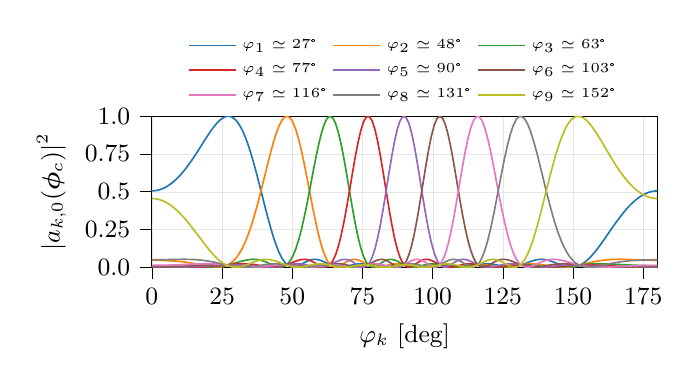
\begin{tikzpicture}

\definecolor{crimson2143940}{RGB}{214,39,40}
\definecolor{darkorange25512714}{RGB}{255,127,14}
\definecolor{forestgreen4416044}{RGB}{44,160,44}
\definecolor{goldenrod18818934}{RGB}{188,189,34}
\definecolor{gray127}{RGB}{127,127,127}
\definecolor{lavender233}{RGB}{233,233,233}
\definecolor{lightgray204}{RGB}{204,204,204}
\definecolor{mediumpurple148103189}{RGB}{148,103,189}
\definecolor{orchid227119194}{RGB}{227,119,194}
\definecolor{sienna1408675}{RGB}{140,86,75}
\definecolor{steelblue31119180}{RGB}{31,119,180}

\begin{axis}[
width=8cm,
height=3.5cm,
legend cell align={left},
legend style={at={(0.5,1.02)}, anchor=south, font=\tiny, draw=none},
legend columns=3,
%transpose legend,
tick align=outside,
tick pos=left,
xlabel={\(\displaystyle \varphi_k\) [deg]},
xmajorgrids,
xmin=0, xmax=180,
xtick={-25,0,25,50,75,100,125,150,175,200},
xticklabels={
  \(\displaystyle {\ensuremath{-}25}\),
  \(\displaystyle {0}\),
  \(\displaystyle {25}\),
  \(\displaystyle {50}\),
  \(\displaystyle {75}\),
  \(\displaystyle {100}\),
  \(\displaystyle {125}\),
  \(\displaystyle {150}\),
  \(\displaystyle {175}\),
  \(\displaystyle {200}\)
},
ylabel={\(\displaystyle |a_{k,0}(\bm{\phi}_c)|^2\)},
ymajorgrids,
ymin=0, ymax=1,
ytick={0,0.25,0.5,0.75,1},
yticklabels={
  \(\displaystyle {0.0}\),
  \(\displaystyle {0.25}\),
  \(\displaystyle {0.5}\),
  \(\displaystyle {0.75}\),
  \(\displaystyle {1.0}\),
}
]
\addplot [semithick, steelblue31119180]
table {%
0 0.505371968059558
1.00558659217877 0.506408608144593
2.01117318435754 0.509519309632246
3.01675977653631 0.514706122818674
4.02234636871508 0.521971484048446
5.02793296089385 0.53131673517447
6.03351955307263 0.542740034080704
7.0391061452514 0.556233644014303
8.04469273743017 0.571780592424018
9.05027932960894 0.589350697884421
10.0558659217877 0.608895977614177
11.0614525139665 0.630345469168378
12.0670391061453 0.653599529050823
13.072625698324 0.678523708933184
14.0782122905028 0.704942357235557
15.0837988826816 0.732632149726398
16.0893854748603 0.761315816547808
17.0949720670391 0.790656402612956
18.1005586592179 0.82025247046676
19.1061452513966 0.849634724748961
20.1117318435754 0.878264599265586
21.1173184357542 0.905535393563618
22.122905027933 0.930776566745304
23.1284916201117 0.953261781804958
24.1340782122905 0.972221233343538
25.1396648044693 0.986858674821584
26.145251396648 0.996373379818496
27.1508379888268 0.99998701943011
28.1564245810056 0.996975113981562
29.1620111731844 0.98670232725067
30.1675977653631 0.968660429097572
31.1731843575419 0.942507281056413
32.1787709497207 0.908104732529133
33.1843575418994 0.8655528961559
34.1899441340782 0.815217951491748
35.195530726257 0.757750463323824
36.2011173184358 0.69409125222153
37.2067039106145 0.625462171575254
38.2122905027933 0.553339764899035
39.2178770949721 0.479410714614247
40.2234636871508 0.405509233242868
41.2290502793296 0.333538036811632
42.2346368715084 0.265376183693859
43.2402234636872 0.202778724528928
44.2458100558659 0.147274619707921
45.2513966480447 0.100070547188386
46.2569832402235 0.0619688484717885
47.2625698324022 0.0333077688033728
48.268156424581 0.0139312120024925
49.2737430167598 0.00319340052751947
50.2793296089386 1.15766218762271e-06
51.2849162011173 0.00289317692215507
52.2905027932961 0.01015189717064
53.2960893854749 0.0199398459917056
54.3016759776536 0.0304490028741272
55.3072625698324 0.0400493398559555
56.3128491620112 0.0474216465575117
57.3184357541899 0.0516603495635942
58.3240223463687 0.0523344229895322
59.3296089385475 0.04949855878036
60.3351955307263 0.0436521722969112
61.340782122905 0.0356499758487714
62.3463687150838 0.0265739940175518
63.3519553072626 0.0175821658874558
64.3575418994413 0.009752259705289
65.3631284916201 0.00394106028156728
66.3687150837989 0.000677313879927379
67.3743016759777 0.000102746296516764
68.3798882681564 0.00196904432664691
69.3854748603352 0.00569083756291851
70.391061452514 0.0104465578189711
71.3966480446927 0.0153118409989782
72.4022346368715 0.0194050568698245
73.4078212290503 0.0220225170870887
74.4134078212291 0.022742380234166
75.4189944134078 0.0214811405133788
76.4245810055866 0.0184941679715897
77.4301675977654 0.0143208798618263
78.4357541899441 0.0096842671565191
79.4413407821229 0.00536211599684286
80.4469273743017 0.00205200392649025
81.4525139664805 0.000253135435489005
82.4581005586592 0.00018507653300445
83.463687150838 0.00175693027169877
84.4692737430168 0.00459158509668591
85.4748603351955 0.00809993995085235
86.4804469273743 0.0115912096101167
87.4860335195531 0.0143991345339076
88.4916201117318 0.0160013031447801
89.4972067039106 0.0161103109582697
90.5027932960894 0.0147208356978718
91.5083798882682 0.0121048940426895
92.5139664804469 0.00875703602585884
93.5195530726257 0.00530026871228962
94.5251396648045 0.0023704266040491
95.5307262569832 0.000500282686486883
96.536312849162 2.43253534198803e-05
97.5418994413408 0.00102096170149574
98.5474860335196 0.00330179687233064
99.5530726256983 0.00644895612218672
100.558659217877 0.00989278644551022
101.564245810056 0.0130152628758377
102.569832402235 0.015260246266761
103.575418994413 0.0162310478267372
104.581005586592 0.015758545311877
105.586592178771 0.0139287326919254
106.59217877095 0.0110659534711147
107.597765363129 0.00767579756874822
108.603351955307 0.00435836958912867
109.608938547486 0.00170724995748734
110.614525139665 0.000211290029394654
111.620111731844 0.000175252229875593
112.625698324022 0.00167158572360081
113.631284916201 0.00453009124420851
114.63687150838 0.00836589998721415
115.642458100559 0.0126401514065036
116.648044692737 0.0167429533789846
117.653631284916 0.0200853182924621
118.659217877095 0.0221861002011615
119.664804469274 0.022741442496056
120.670391061453 0.021667483371579
121.675977653631 0.0191114254235591
122.68156424581 0.015430814511154
123.687150837989 0.011145267824927
124.692737430168 0.00686834455999375
125.698324022346 0.00322936900086494
126.703910614525 0.000795635494134014
127.709497206704 4.61796594339994e-06
128.715083798883 0.00111383361909471
129.720670391061 0.00417325922954661
130.72625698324 0.00902211282298735
131.731843575419 0.0153088237875936
132.737430167598 0.022530480941825
133.743016759777 0.0300862230640983
134.748603351955 0.0373380474672518
135.754189944134 0.0436723651191496
136.759776536313 0.0485562282769491
137.765363128492 0.0515833274291492
138.77094972067 0.052506386985037
139.776536312849 0.0512542643918859
140.782122905028 0.0479336758316469
141.787709497207 0.0428168737030467
142.793296089385 0.0363176780067237
143.798882681564 0.0289589605329934
144.804469273743 0.0213349920734493
145.810055865922 0.0140720239996252
146.815642458101 0.00779015051896706
147.821229050279 0.00306896694881626
148.826815642458 0.000418887194814197
149.832402234637 0.000259289918419415
150.837988826816 0.00290399524892094
151.843575418994 0.00855398381626432
152.849162011173 0.0172967912281748
153.854748603352 0.0291116608183897
154.860335195531 0.0438793177667483
155.86592178771 0.0613951291646616
156.871508379888 0.0813844198671742
157.877094972067 0.103518800987726
158.882681564246 0.127432513028554
159.888268156425 0.152737966064866
160.893854748603 0.179039854842445
161.899441340782 0.20594742041935
162.905027932961 0.233084609469734
163.91061452514 0.260098039030017
164.916201117318 0.286662803442115
165.921787709497 0.312486259839248
166.927374301676 0.337309999484931
167.932960893855 0.360910257098277
168.938547486034 0.383097032665579
169.944134078212 0.40371220428766
170.949720670391 0.422626900689638
171.95530726257 0.439738382206479
172.960893854749 0.454966652966105
173.966480446927 0.468250997717025
174.972067039106 0.479546606698474
175.977653631285 0.488821422930692
176.983240223464 0.496053319514369
177.988826815642 0.501227690666823
178.994413407821 0.504335519521906
180 0.505371968059781
};
\addlegendentry{$\varphi_1 \simeq27$°}
\addplot [semithick, darkorange25512714]
table {%
0 0.046329088038124
1.00558659217877 0.0462605716987796
2.01117318435754 0.0460529592873336
3.01675977653631 0.0457001111713096
4.02234636871508 0.0451919683463674
5.02793296089385 0.0445148312764745
6.03351955307263 0.0436517866800255
7.0391061452514 0.0425833182910534
8.04469273743017 0.0412881471853222
9.05027932960894 0.0397443558774903
10.0558659217877 0.037930857503164
11.0614525139665 0.0358292761215222
12.0670391061453 0.0334263054467838
13.072625698324 0.0307166097703589
14.0782122905028 0.0277063208699055
15.0837988826816 0.0244171665056327
16.0893854748603 0.0208912377808776
17.0949720670391 0.017196362306583
18.1005586592179 0.0134319961641639
19.1061452513966 0.00973547902392744
20.1117318435754 0.00628841327650261
21.1173184357542 0.00332283081388346
22.122905027933 0.00112670305807964
23.1284916201117 4.82361330094407e-05
24.1340782122905 0.000498281492275766
25.1396648044693 0.00295009357053594
26.145251396648 0.00793559382575586
27.1508379888268 0.0160372713141483
28.1564245810056 0.027874882145284
29.1620111731844 0.044086223052019
30.1675977653631 0.0653014660763976
31.1731843575419 0.0921108667209423
32.1787709497207 0.125026105044708
33.1843575418994 0.16443608641301
34.1899441340782 0.210558700962563
35.195530726257 0.263390786939347
36.2011173184358 0.32265931303504
37.2067039106145 0.387777519754847
38.2122905027933 0.457810353420577
39.2178770949721 0.531453889611847
40.2234636871508 0.607033471710209
41.2290502793296 0.682524886895326
42.2346368715084 0.75560198882253
43.2402234636872 0.823712711563589
44.2458100558659 0.884183413449937
45.2513966480447 0.93434901819943
46.2569832402235 0.971703635007812
47.2625698324022 0.994063466145135
48.268156424581 0.999731144607794
49.2737430167598 0.98764852687493
50.2793296089386 0.957523752193232
51.2849162011173 0.909918395980841
52.2905027932961 0.846282036884874
53.2960893854749 0.768924639356974
54.3016759776536 0.680921764620192
55.3072625698324 0.585953494899944
56.3128491620112 0.488084609008591
57.3184357541899 0.391500313646551
58.3240223463687 0.300217914755455
59.3296089385475 0.21779936409069
60.3351955307263 0.14709186375004
61.340782122905 0.0900230722348454
62.3463687150838 0.0474736522442196
63.3519553072626 0.0192430486541022
64.3575418994413 0.00411503540612862
65.3631284916201 1.86864403702759e-05
66.3687150837989 0.00426929758965036
67.3743016759777 0.013863874895731
68.3798882681564 0.0257985427560714
69.3854748603352 0.037371794844291
70.391061452514 0.046438635876347
71.3966480446927 0.0515864524921519
72.4022346368715 0.0522133298848892
73.4078212290503 0.0485022685107469
74.4134078212291 0.0412986177066726
75.4189944134078 0.031911033322495
76.4245810055866 0.0218664314578685
77.4301675977654 0.0126551617193702
78.4357541899441 0.00550301648169024
79.4413407821229 0.0012016112037241
80.4469273743017 1.88777321477881e-05
81.4525139664805 0.0016984495025593
82.4581005586592 0.00554266479471188
83.463687150838 0.010561046662256
84.4692737430168 0.01565651779466
85.4748603351955 0.0198168022726808
86.4804469273743 0.0222791570235175
87.4860335195531 0.0226425194334952
88.4916201117318 0.0209112092519944
89.4972067039106 0.0174666479090806
90.5027932960894 0.0129759674982874
91.5083798882682 0.008256728771075
92.5139664804469 0.00412353350195743
93.5195530726257 0.00124410822704451
94.5251396648045 2.93440106927497e-05
95.5307262569832 0.000574564887735487
96.536312849162 0.00265943300636907
97.5418994413408 0.00580325566856426
98.5474860335196 0.00936296108497901
99.5530726256983 0.012654274418802
100.558659217877 0.0150736894488121
101.564245810056 0.0161999906742632
102.569832402235 0.01585888283713
103.575418994413 0.0141416552700654
104.581005586592 0.0113772863548865
105.586592178771 0.00806542139257457
106.59217877095 0.00478386847681565
107.597765363129 0.00208770555729157
108.603351955307 0.000417388314699408
109.608938547486 3.05833600048099e-05
110.614525139665 0.000967512251758686
111.620111731844 0.00305339893195076
112.625698324022 0.00593531047277286
113.631284916201 0.00914532666849277
114.63687150838 0.0121783668072847
115.642458100559 0.0145715715195883
116.648044692737 0.0159729104909714
117.653631284916 0.0161893259257443
118.659217877095 0.0152086229967294
119.664804469274 0.0131937416469266
120.670391061453 0.010452249109811
121.675977653631 0.00738725950765079
122.68156424581 0.00443809996991752
123.687150837989 0.00201972937362866
124.692737430168 0.000469241540516861
125.698324022346 6.01043795728951e-06
126.703910614525 0.000709549751983815
127.709497206704 0.00251640330744569
128.715083798883 0.00523477430432276
129.720670391061 0.00857347797897635
130.72625698324 0.0121803847749034
131.731843575419 0.0156848998178556
132.737430167598 0.0187391677267668
133.743016759777 0.0210534702722831
134.748603351955 0.0224225054747082
135.754189944134 0.0227406814587269
136.759776536313 0.0220060154270691
137.765363128492 0.0203135203245391
138.77094972067 0.0178399629865328
139.776536312849 0.0148225193996308
140.782122905028 0.0115341221808794
141.787709497207 0.00825822600498787
142.793296089385 0.00526537516922921
143.798882681564 0.00279342907331204
144.804469273743 0.00103267604549248
145.810055865922 0.000116426788491707
146.815642458101 0.000117093878557796
147.821229050279 0.00104728180203947
148.826815642458 0.00286506075626805
149.832402234637 0.00548238535909066
150.837988826816 0.00877553902819433
151.843575418994 0.0125965170419807
152.849162011173 0.0167843801485806
153.854748603352 0.0211757873448919
154.860335195531 0.025614123268198
155.86592178771 0.0299568481228806
156.871508379888 0.0340808968390694
157.877094972067 0.037886125535756
158.882681564246 0.0412969392702313
159.888268156425 0.0442623323966598
160.893854748603 0.0467546325961987
161.899441340782 0.0487672656345947
162.905027932961 0.0503118559141022
163.91061452514 0.0514149545005991
164.916201117318 0.0521146482224944
165.921787709497 0.0524572568406648
166.927374301676 0.0524942754609343
167.932960893855 0.0522796705153013
168.938547486034 0.0518675928460383
169.944134078212 0.0513105326657483
170.949720670391 0.0506579095261757
171.95530726257 0.0499550661731327
172.960893854749 0.0492426180492129
173.966480446927 0.0485560995651779
174.972067039106 0.0479258432036798
175.977653631285 0.0473770270811957
176.983240223464 0.0469298298129761
177.988826815642 0.0465996374944174
178.994413407821 0.0463972556097647
180 0.0463290880381565
};
\addlegendentry{$\varphi_2 \simeq48$°}
\addplot [semithick, forestgreen4416044]
table {%
0 0.01037211066081
1.00558659217877 0.0103258671875362
2.01117318435754 0.0101872049110382
3.01675977653631 0.00995637387196252
4.02234636871508 0.00963394308572096
5.02793296089385 0.00922102966273076
6.03351955307263 0.00871962041633836
7.0391061452514 0.00813298549104426
8.04469273743017 0.0074661815303214
9.05027932960894 0.00672663847472162
10.0558659217877 0.00592481893153242
11.0614525139665 0.00507493193424478
12.0670391061453 0.00419567362917227
13.072625698324 0.00331095593539896
14.0782122905028 0.00245057066733224
15.0837988826816 0.00165072139669604
16.0893854748603 0.000954339222962206
17.0949720670391 0.000411082831668857
18.1005586592179 7.69094619385664e-05
19.1061452513966 1.30939774201967e-05
20.1117318435754 0.000284571003053395
21.1173184357542 0.000957483444466745
22.122905027933 0.0020958433980331
23.1284916201117 0.00375725233095786
24.1340782122905 0.00598768998105283
25.1396648044693 0.00881546831642552
26.145251396648 0.0122445591154183
27.1508379888268 0.0162476398277389
28.1564245810056 0.0207593575469903
29.1620111731844 0.0256704761308801
30.1675977653631 0.0308237327976301
31.1731843575419 0.0360123687092645
32.1787709497207 0.0409823889206739
33.1843575418994 0.0454396224071283
34.1899441340782 0.0490625624589038
35.195530726257 0.0515217423687097
36.2011173184358 0.0525060171350668
37.2067039106145 0.0517555653379414
38.2122905027933 0.0491006990696341
39.2178770949721 0.0445046982821412
40.2234636871508 0.0381079202476765
41.2290502793296 0.0302694555752548
42.2346368715084 0.0216017190099868
43.2402234636872 0.0129927101684463
44.2458100558659 0.00561040521326919
45.2513966480447 0.000883993420570669
46.2569832402235 0.000457579853620839
47.2625698324022 0.00611361915872403
48.268156424581 0.0196657378475845
49.2737430167598 0.0428236622888473
50.2793296089386 0.0770365067466344
51.2849162011173 0.123324385905405
52.2905027932961 0.182111791817308
53.2960893854749 0.253078934383159
54.3016759776536 0.335048779796891
55.3072625698324 0.42592736462812
56.3128491620112 0.522712761547182
57.3184357541899 0.621583666543184
58.3240223463687 0.718072067568704
59.3296089385475 0.807316245638107
60.3351955307263 0.884381166613634
61.340782122905 0.944624131451898
62.3463687150838 0.984075531867625
63.3519553072626 0.999798919996482
64.3575418994413 0.990192433362156
65.3631284916201 0.955195703619808
66.3687150837989 0.896373031112449
67.3743016759777 0.816854547947229
68.3798882681564 0.721131403419341
69.3854748603352 0.614717180839377
70.391061452514 0.503703846243211
71.3966480446927 0.394254386614407
72.4022346368715 0.292083866790011
73.4078212290503 0.201984290777897
74.4134078212291 0.127445478036464
75.4189944134078 0.0704141606307763
76.4245810055866 0.0312176713062822
77.4301675977654 0.00865884141174457
78.4357541899441 0.000267660198013424
79.4413407821229 0.00267578108214886
80.4469273743017 0.0120648917131135
81.4525139664805 0.0246315201139766
82.4581005586592 0.0370103118944929
83.463687150838 0.0466052880830378
84.4692737430168 0.0517929593669801
85.4748603351955 0.0519802435734363
86.4804469273743 0.0475209968044998
87.4860335195531 0.0395144566294492
88.4916201117318 0.0295241015425873
89.4972067039106 0.0192641838402031
90.5027932960894 0.0103024054045695
91.5083798882682 0.00382103066356307
92.5139664804469 0.00046650419531527
93.5195530726257 0.000301620177997394
94.5251396648045 0.00285724454380864
95.5307262569832 0.00726530759159848
96.536312849162 0.0124436042729831
97.5418994413408 0.0172973783267256
98.5474860335196 0.0209032093531169
99.5530726256983 0.0226468028685088
100.558659217877 0.022296453199759
101.564245810056 0.0200061864468184
102.569832402235 0.0162546918187997
103.575418994413 0.0117361205534176
104.581005586592 0.00722521291577041
105.586592178771 0.00344128388497919
106.59217877095 0.000933429537387309
107.597765363129 3.68722478689161e-06
108.603351955307 0.000677074757310245
109.608938547486 0.00271896096647914
110.614525139665 0.00569254652432153
111.620111731844 0.00904353122000405
112.625698324022 0.0121960256552805
113.631284916201 0.0146436202679323
114.63687150838 0.0160219476835726
115.642458100559 0.0161533782312954
116.648044692737 0.0150597654082348
117.653631284916 0.0129444582150033
118.659217877095 0.0101492893941532
119.664804469274 0.00709533902987047
120.670391061453 0.00421766825142007
121.675977653631 0.00190392878449541
122.68156424581 0.000445049969722969
123.687150837989 3.532253825926e-06
124.692737430168 0.000601762655577959
125.698324022346 0.00212972793297489
126.703910614525 0.00436896029448665
127.709497206704 0.00702779452130323
128.715083798883 0.00978217145662639
129.720670391061 0.0123162673207542
130.72625698324 0.0143580161924347
131.731843575419 0.0157059001229888
132.737430167598 0.0162449506121662
133.743016759777 0.0159514888074944
134.748603351955 0.014887524127112
135.754189944134 0.013186788839119
136.759776536313 0.0110350361738521
137.765363128492 0.00864746455934654
138.77094972067 0.00624599722111873
139.776536312849 0.00403872822398931
140.782122905028 0.00220324517553343
141.787709497207 0.000874859058097223
142.793296089385 0.000140105143293841
143.798882681564 3.52972351480309e-05
144.804469273743 0.000549467351935367
145.810055865922 0.00163072622020525
146.815642458101 0.00319493652506109
147.821229050279 0.00513558371728823
148.826815642458 0.00733383024413234
149.832402234637 0.00966791498031588
150.837988826816 0.0120212767221125
151.843575418994 0.0142890086899576
152.849162011173 0.0163824657953231
153.854748603352 0.0182320307766417
154.860335195531 0.0197881891167698
155.86592178771 0.0210211622480253
156.871508379888 0.0219194053799015
157.877094972067 0.0224872954958619
158.882681564246 0.0227423239995605
159.888268156425 0.0227120754271213
160.893854748603 0.0224312267082048
161.899441340782 0.0219387479344988
162.905027932961 0.0212754314413712
163.91061452514 0.0204818256660148
164.916201117318 0.0195966066712952
165.921787709497 0.0186553850073223
166.927374301676 0.0176899192014953
167.932960893855 0.0167276892575854
168.938547486034 0.0157917731530984
169.944134078212 0.0149009651835797
170.949720670391 0.0140700756890759
171.95530726257 0.0133103558393292
172.960893854749 0.0126299974778939
173.966480446927 0.0120346654702258
174.972067039106 0.0115280277224291
175.977653631285 0.0111122554103028
176.983240223464 0.0107884725746496
177.988826815642 0.0105571398730301
178.994413407821 0.0104183618508871
180 0.010372110660771
};
\addlegendentry{$\varphi_3 \simeq63$°}
\addplot [semithick, crimson2143940]
table {%
0 0.00167526583773384
1.00558659217877 0.00165552609164438
2.01117318435754 0.00159692232966114
3.01675977653631 0.00150132069189641
4.02234636871508 0.00137189590932435
5.02793296089385 0.00121322375846471
6.03351955307263 0.00103140167803022
7.0391061452514 0.000834188199558957
8.04469273743017 0.00063114848822041
9.05027932960894 0.000433789542578068
10.0558659217877 0.000255664522764321
11.0614525139665 0.000112421418148779
12.0670391061453 2.17670988478506e-05
13.072625698324 3.31412948989643e-06
14.0782122905028 7.82751180310082e-05
15.0837988826816 0.000268968545818569
16.0893854748603 0.000598101841371227
17.0949720670391 0.00108780289676291
18.1005586592179 0.00175838131024933
19.1061452513966 0.00262681634718431
20.1117318435754 0.00370499073093857
21.1173184357542 0.00499771831285428
22.122905027933 0.00650064923460365
23.1284916201117 0.008198177346884
24.1340782122905 0.0100615192385606
25.1396648044693 0.012047178791866
26.145251396648 0.0140960507727845
27.1508379888268 0.0161334451789809
28.1564245810056 0.0180703232088882
29.1620111731844 0.0198060172917562
30.1675977653631 0.0212326531000855
31.1731843575419 0.0222413934625953
32.1787709497207 0.0227304778026476
33.1843575418994 0.0226148356829256
34.1899441340782 0.0218368149532863
35.195530726257 0.0203772974721656
36.2011173184358 0.0182662011235371
37.2067039106145 0.0155911180928928
38.2122905027933 0.0125026569246554
39.2178770949721 0.00921498660511429
40.2234636871508 0.00600017317860806
41.2290502793296 0.00317519662679069
42.2346368715084 0.00108106815899805
43.2402234636872 5.42435049427759e-05
44.2458100558659 0.000391522490771758
45.2513966480447 0.00231077618655045
46.2569832402235 0.00591104405832843
47.2625698324022 0.011136646721468
48.268156424581 0.0177507834469059
49.2737430167598 0.0253244289983423
50.2793296089386 0.0332460210855952
51.2849162011173 0.0407562866590867
52.2905027932961 0.0470105161910583
53.2960893854749 0.0511676927063013
54.3016759776536 0.0525022851635158
55.3072625698324 0.0505305410344158
56.3128491620112 0.0451392187881568
57.3184357541899 0.0367014539924464
58.3240223463687 0.0261624685501574
59.3296089385475 0.0150776929010086
60.3351955307263 0.00558802488306648
61.340782122905 0.000321610815410449
62.3463687150838 0.00221859611991548
63.3519553072626 0.0142842678168166
64.3575418994413 0.0392860279783683
65.3631284916201 0.0794194944509708
66.3687150837989 0.135977312841179
67.3743016759777 0.209059542659115
68.3798882681564 0.297365501281771
69.3854748603352 0.398102881134326
70.391061452514 0.507040586107346
71.3966480446927 0.61871760181724
72.4022346368715 0.72680264178082
73.4078212290503 0.824580306930747
74.4134078212291 0.905521536593105
75.4189944134078 0.963881833945863
76.4245810055866 0.995262486722366
77.4301675977654 0.997069495291927
78.4357541899441 0.968812902919376
79.4413407821229 0.912205243063546
80.4469273743017 0.831040198073416
81.4525139664805 0.730858566400178
82.4581005586592 0.618434819736982
83.463687150838 0.501140243720594
84.4692737430168 0.386254589952117
85.4748603351955 0.280304897905002
86.4804469273743 0.18850654189349
87.4860335195531 0.114368001497583
88.4916201117318 0.0594992117046345
89.4972067039106 0.0236367076736608
90.5027932960894 0.0048709685283926
91.5083798882682 3.6358505364502e-05
92.5139664804469 0.00520535391622998
93.5195530726257 0.0162187983249176
94.5251396648045 0.0291838223878139
95.5307262569832 0.0408803530549368
96.536312849162 0.0490339742191995
97.5418994413408 0.0524343923054183
98.5474860335196 0.0509014684063186
99.5530726256983 0.0451212969968614
100.558659217877 0.0363903019427302
101.564245810056 0.0263139253600438
102.569832402235 0.0165075488991236
103.575418994413 0.0083413674349638
104.581005586592 0.00275961041613168
105.586592178771 0.000190033172554372
106.59217877095 0.000544491297523424
107.597765363129 0.0032980079512349
108.603351955307 0.00762386476783719
109.608938547486 0.0125569554776577
110.614525139665 0.0171571646146346
111.620111731844 0.0206483272199085
112.625698324022 0.0225152554181616
113.631284916201 0.0225499161870872
114.63687150838 0.0208465856588176
115.642458100559 0.0177533530098093
116.648044692737 0.013792738338564
117.653631284916 0.00956693007330951
118.659217877095 0.00566322084059813
119.664804469274 0.00257301513309063
120.670391061453 0.000633969165078067
121.675977653631 2.09173930199484e-07
122.68156424581 0.000640954840978249
123.687150837989 0.00236391575680042
124.692737430168 0.00485698940063961
125.698324022346 0.00774028697690178
126.703910614525 0.0106203363399998
127.709497206704 0.0131392597015875
128.715083798883 0.01501347466688
129.720670391061 0.0160586432684749
130.72625698324 0.0161998283251133
131.731843575419 0.015467803360076
132.737430167598 0.0139839868938746
133.743016759777 0.0119374228974804
134.748603351955 0.00955759303474808
135.754189944134 0.00708668905275316
136.759776536313 0.00475441535624457
137.765363128492 0.00275757915191073
138.77094972067 0.00124580689910007
139.776536312849 0.000313831474181391
140.782122905028 2.39838537211981e-08
141.787709497207 0.000290260582155958
142.793296089385 0.00112584486509632
143.798882681564 0.00241404621266959
144.804469273743 0.00403983622807684
145.810055865922 0.00587756706770814
146.815642458101 0.0078015888059253
147.821229050279 0.00969510092916627
148.826815642458 0.0114568347746485
149.832402234637 0.0130054377400738
150.837988826816 0.0142816554973123
151.843575418994 0.015248574537193
152.849162011173 0.0158902922386583
153.854748603352 0.016209430055092
154.860335195531 0.0162239065598178
155.86592178771 0.0159633525144039
156.871508379888 0.0154654918070225
157.877094972067 0.0147727412151208
158.882681564246 0.0139292078508513
159.888268156425 0.0129781930564097
160.893854748603 0.0119602503111505
161.899441340782 0.0109117951814215
162.905027932961 0.00986422845670599
163.91061452514 0.00884350899535674
164.916201117318 0.00787009910729055
165.921787709497 0.00695920065458372
166.927374301676 0.00612120233913742
167.932960893855 0.00536226580213062
168.938547486034 0.00468498829374385
169.944134078212 0.00408909121664266
170.949720670391 0.0035720955592564
171.95530726257 0.00312995622713036
172.960893854749 0.00275763696748892
173.966480446927 0.00244961564026774
174.972067039106 0.00220031590406696
175.977653631285 0.00200446599397239
176.983240223464 0.00185738830347994
177.988826815642 0.00175522514640504
178.994413407821 0.00169510658855048
180 0.001675265837739
};
\addlegendentry{$\varphi_4 \simeq77$°}
\addplot [semithick, mediumpurple148103189]
table {%
0 3.50371211491278e-05
1.00558659217877 3.7956285205614e-05
2.01117318435754 4.74116300722816e-05
3.01675977653631 6.54928395415078e-05
4.02234636871508 9.56684268261458e-05
5.02793296089385 0.000142759493390423
6.03351955307263 0.000212893484830375
7.0391061452514 0.000313428686800042
8.04469273743017 0.000452837984963126
9.05027932960894 0.000640538624072977
10.0558659217877 0.000886653560577488
11.0614525139665 0.00120168977892426
12.0670391061453 0.00159611996402554
13.072625698324 0.00207985655470988
14.0782122905028 0.00266161183451654
15.0837988826816 0.00334814470610988
16.0893854748603 0.0041434044313041
17.0949720670391 0.00504759403839742
18.1005586592179 0.00605619120435661
19.1061452513966 0.00715898178450064
20.1117318435754 0.00833917992459865
21.1173184357542 0.00957272747811169
22.122905027933 0.0108278822928848
23.1284916201117 0.0120652172930804
24.1340782122905 0.0132381570666199
25.1396648044693 0.0142941724555817
26.145251396648 0.0151767329125155
27.1508379888268 0.0158280779906171
28.1564245810056 0.016192811044486
29.1620111731844 0.0162222394196128
30.1675977653631 0.0158792878207194
31.1731843575419 0.0151436999673073
32.1787709497207 0.0140171264771365
33.1843575418994 0.0125275864744075
34.1899441340782 0.0107327026762497
35.195530726257 0.00872106346610416
36.2011173184358 0.00661108071980596
37.2067039106145 0.00454680763384202
38.2122905027933 0.00269037077837647
39.2178770949721 0.00121096107835324
40.2234636871508 0.000270713316762906
41.2290502793296 8.26141245762413e-06
42.2346368715084 0.000521247800079368
43.2402234636872 0.00184953251764928
44.2458100558659 0.00396121878534234
45.2513966480447 0.00674380570652463
46.2569832402235 0.0100027149068697
47.2625698324022 0.0134690500419735
48.268156424581 0.016817698762839
49.2737430167598 0.019695782802773
50.2793296089386 0.0217600671735439
51.2849162011173 0.0227203819161154
52.2905027932961 0.0223845797904242
53.2960893854749 0.0206992906083425
54.3016759776536 0.0177800018267164
55.3072625698324 0.013924046953805
56.3128491620112 0.00960111131392529
57.3184357541899 0.00541795493673286
58.3240223463687 0.00205714075502002
59.3296089385475 0.000193399873248908
60.3351955307263 0.000395437321729415
61.340782122905 0.00302489638937183
62.3463687150838 0.00814717488222903
63.3519553072626 0.0154701354565127
64.3575418994413 0.0243258988966143
65.3631284916201 0.0337075131539365
66.3687150837989 0.042366356462858
67.3743016759777 0.0489680826923321
68.3798882681564 0.0522956077190457
69.3854748603352 0.0514782988758557
70.391061452514 0.0462186366642533
71.3966480446927 0.0369826750826025
72.4022346368715 0.0251199267990935
73.4078212290503 0.012882666074864
74.4134078212291 0.00332421473921091
75.4189944134078 6.9876277925745e-05
76.4245810055866 0.00697130437746092
77.4301675977654 0.0276730337996394
78.4357541899441 0.0651360376150526
79.4413407821229 0.121174835796143
80.4469273743017 0.19606958707026
81.4525139664805 0.288311279453759
82.4581005586592 0.394526261011701
83.463687150838 0.509606887303615
84.4692737430168 0.627050231501182
85.4748603351955 0.739479835323908
86.4804469273743 0.83930015781903
87.4860335195531 0.919413473931473
88.4916201117318 0.973917637300646
89.4972067039106 0.998702352808307
90.5027932960894 0.991871889171559
91.5083798882682 0.953942340850237
92.5139664804469 0.887788956671535
93.5195530726257 0.798349908696957
94.5251396648045 0.692122859610875
95.5307262569832 0.576515612638859
96.536312849162 0.459128586723993
97.5418994413408 0.347052739994542
98.5474860335196 0.246261350750725
99.5530726256983 0.16115887394784
100.558659217877 0.0943274446675285
101.564245810056 0.0464849844529584
102.569832402235 0.0166421556754004
103.575418994413 0.00242225823730654
104.581005586592 0.000491470586232651
105.586592178771 0.00703836288748868
106.59217877095 0.0182417984368493
107.597765363129 0.0306743614497623
108.603351955307 0.041602441385049
109.608938547486 0.0491615426200565
110.614525139665 0.0524035315500804
111.620111731844 0.0512288483150905
112.625698324022 0.0462292223138987
113.631284916201 0.038473944309575
114.63687150838 0.0292749240371519
115.642458100559 0.0199630539321713
116.648044692737 0.0117018775609831
117.653631284916 0.00535567060386432
118.659217877095 0.00141933838455233
119.664804469274 8.44275807515524e-06
120.670391061453 0.000900305159508733
121.675977653631 0.00361218365007065
122.68156424581 0.00750023356039651
123.687150837989 0.0118631722524078
124.692737430168 0.0160368062535547
125.698324022346 0.0194691828962891
126.703910614525 0.0217703765886934
127.709497206704 0.0227351401314257
128.715083798883 0.0223403052506227
129.720670391061 0.0207215453271841
130.72625698324 0.0181357515584787
131.731843575419 0.0149158315403145
132.737430167598 0.0114243642034698
133.743016759777 0.00801147370674352
134.748603351955 0.00498079227811258
135.754189944134 0.0025657371723263
136.759776536313 0.000916759420231786
137.765363128492 9.89012984056199e-05
138.77094972067 9.80268950818891e-05
139.776536312849 0.000833502205346037
140.782122905028 0.00217487996479327
141.787709497207 0.00396023282381295
142.793296089385 0.00601409659329599
143.798882681564 0.00816344569304903
144.804469273743 0.0102506428865412
145.810055865922 0.0121428155210749
146.815642458101 0.0137375595039666
147.821229050279 0.0149652282461714
148.826815642458 0.015788312916666
149.832402234637 0.0161985636163978
150.837988826816 0.016212550393181
151.843575418994 0.0158663369615311
152.849162011173 0.0152098599916434
153.854748603352 0.0143014941417434
154.860335195531 0.0132031564752997
155.86592178771 0.011976178678156
156.871508379888 0.0106780625224926
157.877094972067 0.00936014008492376
158.882681564246 0.0080660884748743
159.888268156425 0.00683119947177741
160.893854748603 0.00568227564641977
161.899441340782 0.00463801305548458
162.905027932961 0.00370973264736563
163.91061452514 0.00290233419977525
164.916201117318 0.00221536433333133
165.921787709497 0.0016441108392568
166.927374301676 0.00118065681856501
167.932960893855 0.000814848191832945
168.938547486034 0.000535145874387739
169.944134078212 0.000329348698712827
170.949720670391 0.000185184804613867
171.95530726257 9.07778007947723e-05
172.960893854749 3.49998253302915e-05
173.966480446927 7.72709884500054e-06
174.972067039106 1.51184476217865e-08
175.977653631285 4.21071780908316e-06
176.983240223464 1.40172132567171e-05
177.988826815642 2.45270987140469e-05
178.994413407821 3.22345075285129e-05
180 3.5037121151691e-05
};
\addlegendentry{$\varphi_5 \simeq90$°}
\addplot [semithick, sienna1408675]
table {%
0 0.00275795373031666
1.00558659217877 0.00278228728541802
2.01117318435754 0.00285577108902419
3.01675977653631 0.00297982924291646
4.02234636871508 0.00315675015315515
5.02793296089385 0.0033895564657555
6.03351955307263 0.00368181850044143
7.0391061452514 0.004037407559323
8.04469273743017 0.00446018568199644
9.05027932960894 0.00495362955428851
10.0558659217877 0.00552038856016708
11.0614525139665 0.00616178058338612
12.0670391061453 0.00687723425576652
13.072625698324 0.00766369297100412
14.0782122905028 0.00851500407647164
15.0837988826816 0.0094213259907997
16.0893854748603 0.0103685961313986
17.0949720670391 0.0113381127651937
18.1005586592179 0.0123062932271683
19.1061452513966 0.0132446780709932
20.1117318435754 0.0141202540499421
21.1173184357542 0.0148961665578007
22.122905027933 0.0155328824143016
23.1284916201117 0.015989844862955
24.1340782122905 0.0162276329692067
25.1396648044693 0.0162105965514214
26.145251396648 0.0159098857407453
27.1508379888268 0.0153067330892096
28.1564245810056 0.014395779496121
29.1620111731844 0.0131881687893735
30.1675977653631 0.0117140773477366
31.1731843575419 0.0100243042467369
32.1787709497207 0.00819053481555115
33.1843575418994 0.00630391709857414
34.1899441340782 0.00447166609492539
35.195530726257 0.00281154121312196
36.2011173184358 0.00144422929689325
37.2067039106145 0.000483902809216653
38.2122905027933 2.74953295438577e-05
39.2178770949721 0.000143519703636316
40.2234636871508 0.000861513842350861
41.2290502793296 0.00216339372340421
42.2346368715084 0.00397807745754953
43.2402234636872 0.00618067537701994
44.2458100558659 0.00859728556511188
45.2513966480447 0.0110159764115128
46.2569832402235 0.0132038877267616
47.2625698324022 0.0149295817440664
48.268156424581 0.0159889018242423
49.2737430167598 0.0162317593138985
50.2793296089386 0.0155866013516928
51.2849162011173 0.0140789570218178
52.2905027932961 0.0118405464196267
53.2960893854749 0.00910605984037092
54.3016759776536 0.00619590215830709
55.3072625698324 0.00348489537258632
56.3128491620112 0.00135898763187006
57.3184357541899 0.000164181296358684
58.3240223463687 0.000153840617626448
59.3296089385475 0.00144190775735018
60.3351955307263 0.00396999668988544
61.340782122905 0.00749558206077358
62.3463687150838 0.0116064357703747
63.3519553072626 0.0157631711644155
64.3575418994413 0.0193675477082004
65.3631284916201 0.0218496066935436
66.3687150837989 0.0227624637819307
67.3743016759777 0.0218704705132796
68.3798882681564 0.0192152203439093
69.3854748603352 0.0151450686537385
70.391061452514 0.010297683494548
71.3966480446927 0.00553143519723414
72.4022346368715 0.00180948662632673
73.4078212290503 4.91495521110927e-05
74.4134078212291 0.000957013079827847
75.4189944134078 0.00487602123402655
76.4245810055866 0.0116727388777012
77.4301675977654 0.0206905935916301
78.4357541899441 0.0307876748482924
79.4413407821229 0.0404662712142377
80.4469273743017 0.0480871021236943
81.4525139664805 0.0521461945417169
82.4581005586592 0.051578998840688
83.463687150838 0.0460470706700976
84.4692737430168 0.0361594817186801
85.4748603351955 0.023585256809553
86.4804469273743 0.0110246531371018
87.4860335195531 0.002024859052884
88.4916201117318 0.000647419712967359
89.4972067039106 0.0110172853089791
90.5027932960894 0.0368033470800797
91.5083798882682 0.0806943927477055
92.5139664804469 0.143940044457549
93.5195530726257 0.226022115301474
94.5251396648045 0.324508088599827
95.5307262569832 0.435116744519964
96.536312849162 0.551999265871643
97.5418994413408 0.668211216058013
98.5474860335196 0.776325608444251
99.5530726256983 0.869118501213818
100.558659217877 0.940248824596267
101.564245810056 0.98485478755923
102.569832402235 0.999999989142516
103.575418994413 0.984921578771085
104.581005586592 0.941057609204994
105.586592178771 0.871857555303068
106.59217877095 0.782405153763619
107.597765363129 0.678902999378293
108.603351955307 0.56808133441773
109.608938547486 0.456597976405747
110.614525139665 0.350492386451294
111.620111731844 0.254745673023022
112.625698324022 0.172981918847015
113.631284916201 0.107327177806365
114.63687150838 0.0584234711286252
115.642458100559 0.0255784850699714
116.648044692737 0.007019218517049
117.653631284916 0.000210572399104093
118.659217877095 0.00219803499841121
119.664804469274 0.0099366941767578
120.670391061453 0.0205757385617813
121.675977653631 0.0316770003016157
122.68156424581 0.0413564492363337
123.687150837989 0.0483474933710919
124.692737430168 0.0519933704098796
125.698324022346 0.0521820998079124
126.703910614525 0.0492410765958535
127.709497206704 0.0438094716792772
128.715083798883 0.0367055007787828
129.720670391061 0.0288028760921831
130.72625698324 0.0209269930901093
131.731843575419 0.0137772560286586
132.737430167598 0.00787795416938826
133.743016759777 0.00355667889766847
134.748603351955 0.000946678493725625
135.754189944134 7.88903310857864e-06
136.759776536313 0.000560632785331702
137.765363128492 0.00232601726871606
138.77094972067 0.00496771546117817
139.776536312849 0.00813085204193639
140.782122905028 0.0114749586012832
141.787709497207 0.014699216586232
142.793296089385 0.0175593452974639
143.798882681564 0.0198764244626791
144.804469273743 0.0215386221244689
145.810055865922 0.0224972221095745
146.815642458101 0.022758533344126
147.821229050279 0.0223732567234692
148.826815642458 0.0214247344569427
149.832402234637 0.0200172635381909
150.837988826816 0.0182653665183127
151.843575418994 0.0162846181260244
152.849162011173 0.0141843545350215
153.854748603352 0.0120623620580532
154.860335195531 0.0100014633749672
155.86592178771 0.00806779411380638
156.871508379888 0.00631048717276591
157.877094972067 0.00476244943123828
158.882681564246 0.00344191644021275
159.888268156425 0.00235449583716069
160.893854748603 0.00149545072636898
161.899441340782 0.000852022468719845
162.905027932961 0.000405642171482451
163.91061452514 0.000133927257291739
164.916201117318 1.24009524317463e-05
165.921787709497 1.59068314092188e-05
166.927374301676 0.000119717196839826
167.932960893855 0.000300353338219873
168.938547486034 0.000536148379593192
169.944134078212 0.000807590553140769
170.949720670391 0.00109748748445012
171.95530726257 0.00139099158167673
172.960893854749 0.00167552390953364
173.966480446927 0.00194062986917327
174.972067039106 0.00217779528734474
175.977653631285 0.00238024665703537
176.983240223464 0.00254275462440922
177.988826815642 0.00266145559512631
178.994413407821 0.00273370264065498
180 0.00275795373030967
};
\addlegendentry{$\varphi_6 \simeq103$°}
\addplot [semithick, orchid227119194]
table {%
0 0.0126305937689744
1.00558659217877 0.0126763074318849
2.01117318435754 0.0128132555339679
3.01675977653631 0.013040816747748
4.02234636871508 0.0133578144095521
5.02793296089385 0.013762308847843
6.03351955307263 0.0142513150885622
7.0391061452514 0.0148204553637751
8.04469273743017 0.0154635598520546
9.05027932960894 0.0161722338935513
10.0558659217877 0.016935415539316
11.0614525139665 0.0177389535663276
12.0670391061453 0.0185652427215091
13.072625698324 0.0193929594787529
14.0782122905028 0.020196947322943
15.0837988826816 0.0209483046460655
16.0893854748603 0.0216147297057628
17.0949720670391 0.0221611745544353
18.1005586592179 0.0225508521616074
19.1061452513966 0.0227466269330579
20.1117318435754 0.0227127975213353
21.1173184357542 0.0224172516929433
22.122905027933 0.0218339362048751
23.1284916201117 0.0209455411772811
24.1340782122905 0.0197462505153675
25.1396648044693 0.0182443609985964
26.145251396648 0.016464527577904
27.1508379888268 0.0144493573283941
28.1564245810056 0.0122600565104902
29.1620111731844 0.00997584183042332
30.1675977653631 0.00769186541529065
31.1731843575419 0.00551547888735412
32.1787709497207 0.00356077815499267
33.1843575418994 0.0019415259344529
34.1899441340782 0.000762737010531837
35.195530726257 0.000111418970646543
36.2011173184358 4.71691185505811e-05
37.2067039106145 0.000593510929958938
38.2122905027933 0.00173098076244435
39.2178770949721 0.00339301605609963
40.2234636871508 0.0054656209897422
41.2290502793296 0.00779157313103176
42.2346368715084 0.0101795767673909
43.2402234636872 0.0124182753430102
44.2458100558659 0.01429443892155
45.2513966480447 0.0156139986860239
46.2569832402235 0.0162239868083991
47.2625698324022 0.0160329499610285
48.268156424581 0.0150271370730538
49.2737430167598 0.0132798065029974
50.2793296089386 0.0109514187426607
51.2849162011173 0.00827929940875188
52.2905027932961 0.00555653778167369
53.2960893854749 0.00310132716461134
54.3016759776536 0.00121948897547407
55.3072625698324 0.000164334784002186
56.3128491620112 9.90643012673486e-05
57.3184357541899 0.00106733596492514
58.3240223463687 0.00297729487663237
59.3296089385475 0.00560310983421517
60.3351955307263 0.00860599736076604
61.340782122905 0.0115739874265712
62.3463687150838 0.0140766523799025
63.3519553072626 0.0157281334832875
64.3575418994413 0.0162495714792857
65.3631284916201 0.0155209666732684
66.3687150837989 0.0136129290057552
67.3743016759777 0.0107908901955563
68.3798882681564 0.00748802442524845
69.3854748603352 0.00424794691780075
70.391061452514 0.00164354338619828
71.3966480446927 0.00018315088238309
72.4022346368715 0.000218830902181223
73.4078212290503 0.00187283051388923
74.4134078212291 0.00499698306019677
75.4189944134078 0.00917564983930161
76.4245810055866 0.0137762486027235
77.4301675977654 0.0180433545819035
78.4357541899441 0.0212240909931125
79.4413407821229 0.0227055433112218
80.4469273743017 0.0221406686686124
81.4525139664805 0.0195387210394376
82.4581005586592 0.0153000791269284
83.463687150838 0.0101833033897679
84.4692737430168 0.00520323607119375
85.4748603351955 0.00147130034936055
86.4804469273743 7.44224274786155e-07
87.4860335195531 0.00150824515952699
88.4916201117318 0.00624721548608887
89.4972067039106 0.013906203736657
90.5027932960894 0.0235978167316281
91.5083798882682 0.0339504987812529
92.5139664804469 0.0432991760290533
93.5195530726257 0.049953776751022
94.5251396648045 0.052509816282755
95.5307262569832 0.0501552159276693
96.536312849162 0.0429242500449167
97.5418994413408 0.0318538759808609
98.5474860335196 0.0190093514727298
99.5530726256983 0.00736342599089224
100.558659217877 0.000533974596143985
101.564245810056 0.00240562783630718
102.569832402235 0.0166785818562629
103.575418994413 0.0463996469982013
104.581005586592 0.0935348965356593
105.586592178771 0.158639362342358
106.59217877095 0.240667690934757
107.597765363129 0.336952243649963
108.603351955307 0.443354342585843
109.608938547486 0.55457317615385
110.614525139665 0.664578173111623
111.620111731844 0.767116835349336
112.625698324022 0.856242681739457
113.631284916201 0.92680770402021
114.63687150838 0.974870173144353
115.642458100559 0.997980494177316
116.648044692737 0.995323206260202
117.653631284916 0.967709978501232
118.659217877095 0.917434409498913
119.664804469274 0.848012761964294
120.670391061453 0.763844147580561
121.675977653631 0.66982845325472
122.68156424581 0.570980448480929
123.687150837989 0.472074580824214
124.692737430168 0.377347917839802
125.698324022346 0.290279731273728
126.703910614525 0.21345659678088
127.709497206704 0.148522741118481
128.715083798883 0.0962076163113191
129.720670391061 0.0564169186873155
130.72625698324 0.0283697768474501
131.731843575419 0.0107635828103837
132.737430167598 0.00194866826096638
133.743016759777 9.73002752390577e-05
134.748603351955 0.00335477110470468
135.754189944134 0.0099641589831519
136.759776536313 0.0183601682688837
137.765363128492 0.0272309386244852
138.77094972067 0.0355495814296478
139.776536312849 0.0425793136718492
140.782122905028 0.0478573798706243
141.787709497207 0.051163533231908
142.793296089385 0.0524788017836205
143.798882681564 0.0519397422765541
144.804469273743 0.0497925438214962
145.810055865922 0.0463503361670201
146.815642458101 0.0419560142845826
147.821229050279 0.0369519124259125
148.826815642458 0.0316568162156511
149.832402234637 0.0263501295591828
150.837988826816 0.0212625270247178
151.843575418994 0.0165721145076962
152.849162011173 0.0124049699664475
153.854748603352 0.00883891227937555
154.860335195531 0.00590941720716547
155.86592178771 0.00361673328861403
156.871508379888 0.00193341901040744
157.877094972067 0.000811702627928986
158.882681564246 0.000190240109715929
159.888268156425 2.94906868823924e-09
160.893854748603 0.000169159098110182
161.899441340782 0.000626914186723159
162.905027932961 0.00130635672026042
163.91061452514 0.00214640246544444
164.916201117318 0.00309296335642282
165.921787709497 0.00409947917925834
166.927374301676 0.00512695026446335
167.932960893855 0.00614360035672014
168.938547486034 0.00712428413457795
169.944134078212 0.00804973627134943
170.949720670391 0.00890574058206734
171.95530726257 0.00968228018608383
172.960893854749 0.0103727137226613
173.966480446927 0.0109730090418016
174.972067039106 0.0114810546793042
175.977653631285 0.0118960608074819
176.983240223464 0.0122180550576742
177.988826815642 0.0124474743671201
178.994413407821 0.0125848514981056
180 0.0126305937690159
};
\addlegendentry{$\varphi_7 \simeq116$°}
\addplot [semithick, gray127]
table {%
0 0.0492432762805038
1.00558659217877 0.0492935627745562
2.01117318435754 0.0494421310256901
3.01675977653631 0.0496820849604594
4.02234636871508 0.0500018618849924
5.02793296089385 0.0503851472532138
6.03351955307263 0.0508107920859005
7.0391061452514 0.0512527685541826
8.04469273743017 0.0516802074487779
9.05027932960894 0.0520575677772819
10.0558659217877 0.0523449928810093
11.0614525139665 0.0524989085402917
12.0670391061453 0.0524729156856318
13.072625698324 0.0522190227155852
14.0782122905028 0.05168924922854
15.0837988826816 0.0508376135704038
16.0893854748603 0.049622490597975
17.0949720670391 0.0480092935778956
18.1005586592179 0.0459733958381092
19.1061452513966 0.0435031651692245
20.1117318435754 0.0406029393923296
21.1173184357542 0.0372957283677152
22.122905027933 0.0336253904008791
23.1284916201117 0.0296580047773254
24.1340782122905 0.0254821529198856
25.1396648044693 0.0212078344741826
26.145251396648 0.0169637870724696
27.1508379888268 0.0128930539238786
28.1564245810056 0.00914675381296489
29.1620111731844 0.00587615240711855
30.1675977653631 0.00322330665652807
31.1731843575419 0.00131074528942386
32.1787709497207 0.000230842499966566
33.1843575418994 3.57184777602492e-05
34.1899441340782 0.00072863507564328
35.195530726257 0.00225792129341101
36.2011173184358 0.00451443582495291
37.2067039106145 0.00733343159775423
38.2122905027933 0.0105014175830137
39.2178770949721 0.0137682165932661
40.2234636871508 0.0168639112676809
41.2290502793296 0.0195197897979232
42.2346368715084 0.0214918030957531
43.2402234636872 0.0225844974670887
44.2458100558659 0.0226729734944862
45.2513966480447 0.0217202262601214
46.2569832402235 0.0197873172844504
47.2625698324022 0.0170342635442791
48.268156424581 0.0137103151484516
49.2737430167598 0.0101333937732729
50.2793296089386 0.00665978767623467
51.2849162011173 0.00364660222773806
52.2905027932961 0.00141076159375864
53.2960893854749 0.000189339877734812
54.3016759776536 0.000106467948212407
55.3072625698324 0.00115185562514868
56.3128491620112 0.00317500392261588
57.3184357541899 0.00589747977424855
58.3240223463687 0.00894332956504347
59.3296089385475 0.0118850830012572
60.3351955307263 0.0143002098348823
61.340782122905 0.0158307579539305
62.3463687150838 0.0162376333363808
63.3519553072626 0.0154409097070248
64.3575418994413 0.0135388543089364
65.3631284916201 0.0108009920001531
66.3687150837989 0.00763423180394671
67.3743016759777 0.00452535223119575
68.3798882681564 0.00196732016162635
69.3854748603352 0.000380267816184444
70.391061452514 3.97928240094368e-05
71.3966480446927 0.00102508502712733
72.4022346368715 0.00319703245137494
73.4078212290503 0.00621210830340269
74.4134078212291 0.00957207055695405
75.4189944134078 0.0127032208850486
76.4245810055866 0.0150532663806801
77.4301675977654 0.0161898043908833
78.4357541899441 0.0158829992123455
79.4413407821229 0.0141566310300647
80.4469273743017 0.0112963304603882
81.4525139664805 0.00781084897893379
82.4581005586592 0.0043505308286316
83.463687150838 0.00159528613954165
84.4692737430168 0.000130779428806431
85.4748603351955 0.000334916700857471
86.4804469273743 0.00229619768394048
87.4860335195531 0.00578093910724082
88.4916201117318 0.0102583703910284
89.4972067039106 0.0149824450291127
90.5027932960894 0.0191186725699423
91.5083798882682 0.021895300389783
92.5139664804469 0.0227525116056145
93.5195530726257 0.0214621709787877
94.5251396648045 0.0181944720206712
95.5307262569832 0.0135161437491955
96.536312849162 0.00831634976824421
97.5418994413408 0.00366911582324254
98.5474860335196 0.000652831264937274
99.5530726256983 0.00015597832699078
100.558659217877 0.00270214563209499
101.564245810056 0.00832577085102995
102.569832402235 0.0165230723744102
103.575418994413 0.0262913396008299
104.581005586592 0.0362559655402197
105.586592178771 0.0448705582832274
106.59217877095 0.0506634329713996
107.597765363129 0.0524956916207823
108.603351955307 0.0497932134824129
109.608938547486 0.0427176212530869
110.614525139665 0.032249183363324
111.620111731844 0.0201664008721325
112.625698324022 0.00892089852285482
113.631284916201 0.00142013967516408
114.63687150838 0.000742446616830047
115.642458100559 0.00981724316219364
116.648044692737 0.0311073499051865
117.653631284916 0.0663292558723775
118.659217877095 0.116241952861857
119.664804469274 0.18052611476848
120.670391061453 0.257764486212133
121.675977653631 0.345522828869125
122.68156424581 0.440520115471861
123.687150837989 0.538868065136932
124.692737430168 0.636354400840507
125.698324022346 0.728741756044869
126.703910614525 0.812054898571209
127.709497206704 0.882832437159138
128.715083798883 0.938324721899872
129.720670391061 0.97662639235927
130.72625698324 0.996739096206071
131.731843575419 0.998566514753151
132.737430167598 0.9828493754518
133.743016759777 0.951052202512444
134.748603351955 0.905215975600858
135.754189944134 0.84779165767001
136.759776536313 0.781468906414289
137.765363128492 0.709012503505663
138.77094972067 0.633116484977502
139.776536312849 0.556283006975732
140.782122905028 0.480729973408881
141.787709497207 0.408328664396346
142.793296089385 0.340570238143575
143.798882681564 0.27855815424659
144.804469273743 0.223022327957794
145.810055865922 0.174350154053493
146.815642458101 0.132629369990063
147.821229050279 0.0976979654413116
148.826815642458 0.069196879835297
149.832402234637 0.0466219516318279
150.837988826816 0.0293723932872744
151.843575418994 0.0167938812330965
152.849162011173 0.00821510771181583
153.854748603352 0.00297729841016605
154.860335195531 0.000456732769492333
155.86592178771 8.07049363177386e-05
156.871508379888 0.00133763717159105
157.877094972067 0.0037822174839813
158.882681564246 0.0070364977619256
159.888268156425 0.0107878784571697
160.893854748603 0.014784841536402
161.899441340782 0.0188311938748453
162.905027932961 0.0227794646918623
163.91061452514 0.0265239760055676
164.916201117318 0.029993984111112
165.921787709497 0.0331471794203639
166.927374301676 0.0359637356553833
167.932960893855 0.0384410192183086
168.938547486034 0.0405890057986892
169.944134078212 0.042426403005894
170.949720670391 0.0439774433623612
171.95530726257 0.0452692893483643
172.960893854749 0.0463299791807385
173.966480446927 0.047186836562363
174.972067039106 0.0478652678806978
175.977653631285 0.0483878746400664
176.983240223464 0.0487738159628285
177.988826815642 0.0490383647909272
178.994413407821 0.0491926111737391
180 0.0492432762804642
};
\addlegendentry{$\varphi_8 \simeq131$°}
\addplot [semithick, goldenrod18818934]
table {%
0 0.454953333164848
1.00558659217877 0.453932081085003
2.01117318435754 0.450871218207153
3.01675977653631 0.445779692846949
4.02234636871508 0.438673306152156
5.02793296089385 0.429576018818503
6.03351955307263 0.418521730732028
7.0391061452514 0.405556480814793
8.04469273743017 0.390740995342162
9.05027932960894 0.3741534915394
10.0558659217877 0.355892619427203
11.0614525139665 0.336080399071876
12.0670391061453 0.31486498347619
13.072625698324 0.29242305072144
14.0782122905028 0.268961604547019
15.0837988826816 0.244718942877701
16.0893854748603 0.219964541917266
17.0949720670391 0.194997602862152
18.1005586592179 0.170144022833063
19.1061452513966 0.145751585166628
20.1117318435754 0.122183220204828
21.1173184357542 0.0998082689575708
22.122905027933 0.0789917898149839
23.1284916201117 0.0600820823081412
24.1340782122905 0.0433967585733338
25.1396648044693 0.0292078663355091
26.145251396648 0.0177267469967193
27.1508379888268 0.0090894851132329
28.1564245810056 0.00334395401401186
29.1620111731844 0.00043956650250972
30.1675977653631 0.000220877961536594
31.1731843575419 0.00242614054553398
32.1787709497207 0.00669175320898292
33.1843575418994 0.0125632806735865
34.1899441340782 0.0195133218017579
35.195530726257 0.0269660031953826
36.2011173184358 0.0343272809416358
37.2067039106145 0.0410195922540271
38.2122905027933 0.0465187651549604
39.2178770949721 0.0503905375451018
40.2234636871508 0.0523236345190581
41.2290502793296 0.0521561827065291
42.2346368715084 0.0498923714749009
43.2402234636872 0.0457067509113038
44.2458100558659 0.0399344010469456
45.2513966480447 0.0330463886974511
46.2569832402235 0.0256113713835979
47.2625698324022 0.018245785768604
48.268156424581 0.0115566006532686
49.2737430167598 0.00608192192779357
50.2793296089386 0.00223560166118849
51.2849162011173 0.000262239522375192
52.2905027932961 0.000208438705151684
53.2960893854749 0.00191484067179322
54.3016759776536 0.00503137095255579
55.3072625698324 0.0090554587112937
56.3128491620112 0.0133900366237571
57.3184357541899 0.0174152648590824
58.3240223463687 0.0205655785372642
59.3296089385475 0.0224022415900702
60.3351955307263 0.0226714272456461
61.340782122905 0.0213391118014879
62.3463687150838 0.0185967370028931
63.3519553072626 0.0148354121729149
64.3575418994413 0.0105909172586766
65.3631284916201 0.00646629114185995
66.3687150837989 0.00304262419512869
67.3743016759777 0.00079113209984596
68.3798882681564 1.39145984375555e-07
69.3854748603352 0.000728983398373575
70.391061452514 0.00279716013354819
71.3966480446927 0.00581170060913907
72.4022346368715 0.00922962392380339
73.4078212290503 0.0124463013764774
74.4134078212291 0.014895791888684
75.4189944134078 0.0161465666877229
76.4245810055866 0.0159761483628136
77.4301675977654 0.0144111947417847
78.4357541899441 0.011725092678427
79.4413407821229 0.00839233152516395
80.4469273743017 0.00500657876196263
81.4525139664805 0.00217610352075885
82.4581005586592 0.000414707354103969
83.463687150838 4.76929200847921e-05
84.4692737430168 0.0011502434821859
85.4748603351955 0.00353016091751855
86.4804469273743 0.00675910828007346
87.4860335195531 0.0102477013823806
88.4916201117318 0.0133516084405068
89.4972067039106 0.0154898000538547
90.5027932960894 0.0162534306144609
91.5083798882682 0.0154851080489432
92.5139664804469 0.0133133695237498
93.5195530726257 0.010135153589941
94.5251396648045 0.00654850480600553
95.5307262569832 0.00324692640645368
96.536312849162 0.000894000832725242
97.5418994413408 7.72985609372953e-07
98.5474860335196 0.00082819680353391
99.5530726256983 0.00333269635781373
100.558659217877 0.00716535185463321
101.564245810056 0.0117257548100741
102.569832402235 0.0162618939812238
103.575418994413 0.0199992660589392
104.581005586592 0.022277189733844
105.586592178771 0.0226689260847186
106.59217877095 0.021064864000451
107.597765363129 0.0177041979841107
108.603351955307 0.0131490932255568
109.608938547486 0.00820480663521554
110.614525139665 0.00379801547472756
111.620111731844 0.000832274176727218
112.625698324022 4.3058761037622e-05
113.631284916201 0.00187480662370172
114.63687150838 0.00639885750907765
115.642458100559 0.0132849301441156
116.648044692737 0.0218308048034424
117.653631284916 0.0310464979916154
118.659217877095 0.0397816665326033
119.664804469274 0.0468793088688479
120.670391061453 0.0513357329953862
121.675977653631 0.0524464994416578
122.68156424581 0.0499204649236647
123.687150837989 0.0439486278810557
124.692737430168 0.0352204421023292
125.698324022346 0.0248867362169964
126.703910614525 0.0144744939869015
127.709497206704 0.00576378908062666
128.715083798883 0.000640622374643691
129.720670391061 0.000941031178420766
130.72625698324 0.00830163559863792
131.731843575419 0.0240299851792533
132.737430167598 0.0490050571006932
133.743016759777 0.0836145125959564
134.748603351955 0.127731335171741
135.754189944134 0.180728702360369
136.759776536313 0.241528741144575
137.765363128492 0.308678427672367
138.77094972067 0.380444431207745
139.776536312849 0.45491817093874
140.782122905028 0.530122657217107
141.787709497207 0.604113663227344
142.793296089385 0.675069218666004
143.798882681564 0.741363123934669
144.804469273743 0.801619956129767
145.810055865922 0.854750712341651
146.815642458101 0.899969688247686
147.821229050279 0.936794342254477
148.826815642458 0.965030711702416
149.832402234637 0.984747428982127
150.837988826816 0.996241561479808
151.843575418994 0.999999419105002
152.849162011173 0.996655196346883
153.854748603352 0.986949904660174
154.860335195531 0.971692564471408
155.86592178771 0.951725115521153
156.871508379888 0.927892010790485
157.877094972067 0.901015012985174
158.882681564246 0.871873332763325
159.888268156425 0.841188944286609
160.893854748603 0.809616687999107
161.899441340782 0.777738618568935
162.905027932961 0.746061969309716
163.91061452514 0.715020072409164
164.916201117318 0.68497558527983
165.921787709497 0.656225415803369
166.927374301676 0.629006802622081
167.932960893855 0.603504081872188
168.938547486034 0.579855751371394
169.944134078212 0.558161521624677
170.949720670391 0.538489115953783
171.95530726257 0.52088064693133
172.960893854749 0.505358451654269
173.966480446927 0.491930313651374
174.972067039106 0.480594034569528
175.977653631285 0.471341344867432
176.983240223464 0.464161160529893
177.988826815642 0.459042203420924
178.994413407821 0.455975007523751
180 0.454953333164632
};
\addlegendentry{$\varphi_{9} \simeq152$°}
\end{axis}

\end{tikzpicture}

    \caption{Visualization of the \gls{AF} using the codebook design in~\eqref{eq:codebook-design}, with $\tau = 0.5$, $x_\tau = 1.391$, and $N_x=8$.}
    \label{fig:codebook-design}
\end{figure}

\section{Resource allocation} \label{sec:scheduling}
In this section, we present the allocation scheduling process based on the proposed framework.

Given the set of configurations $\mc{C}$, the set of available of \glspl{RB}, and the position information of each user, 
we know the value of the deterministic part of the \gls{SNR} for all the \glspl{UE}, \glspl{RB} and time-slots. Nevertheless, the actual \gls{SNR} is a random variable: to provide a feasible communication rate, the \gls{SE} set for the data transmission must be lower than the achievable capacity. 
%Let us define $\epsilon$ as the probability of success of sending data in any time-frequency resource. 
To overcome this issue, we define the $\epsilon$-robust \gls{SE} $r_{k,f,c}^\epsilon$ as the \gls{SE} that assures that the data transmitted by \gls{UE} $k$ on \gls{RB} $f$ and under configuration $c\in\mc{C}$ are successfully decoded with probability $\epsilon$, i.e., the \gls{SE} satisfying
\begin{equation}
    \mc{P}\left[r_{k,f,c}^\epsilon \le \log_2\left( 1 + \gamma_{k,f,c}\right) \right] \le 1 - \epsilon.
\end{equation}
%The value of $r_{k,f,c}^\epsilon$ is given by the following Lemma.
\begin{lemma}
Following Assumption~\ref{assu:channel}, the  $\epsilon$-robust \gls{SE} is
\begin{equation}
    r_{k,f,c}^\epsilon = \log_2\left(1 + \frac{P_k}{2\sigma^2(\kappa +1)} F^{-1}_{\tilde{\gamma}_{k,f,c}}(1 - \epsilon) \right)
\end{equation}
where $F^{-1}_{\tilde{\gamma}_{k,f,c}}(\cdot)$ is the inverse \gls{CDF} function of $\tilde{\gamma}_{k,f,c} \sim \chi_2^{2}(\xi_{k,f,c})$, where $\xi_{k,f,c}$ is given in eq.~\eqref{eq:nc} at the top of next page.
\end{lemma}
%
\begin{figure*}[bt]
    \centering
\begin{equation} \label{eq:nc}
\xi_{k,f,c} = 2\left(\kappa + \frac{\kappa + 1}{\beta(r_{b,k})} |g_{f,k}(\mb{\phi}_c)|^2 + 2 \sqrt{\frac{\kappa + 1}{\beta(r_{b,k})}} \Re\{ d_{f}(r_{k,b}) g_{k,f}(\mb{\phi}_c)\} \right)
\end{equation}
\par\noindent\rule{\textwidth}{0.4pt}
\end{figure*}
%
\begin{proof}
The proof comes directly from the definition of the channels~\eqref{eq:channel:direct}-\eqref{eq:channel:reflected} after few manipulations. %, we have $h_{k,f} + g_{k,f}(\bm{\phi}_c) \sim \mc{CN}(\sqrt{\beta_k(r_{b,k}) \kappa / (\kappa + 1)} d_{f} + g_{k,f}, \beta_k(r_{b,k}) / (\kappa + 1))$. 
\end{proof}

In practice, knowing the deterministic part of the \gls{SNR} allows us to compute the $\epsilon$-robust \gls{SE} for all the resources and use it to optimize the allocation.
To this purpose, we further define the allocation variable $\rho_{k,f,c}\in\{0,1\}$, mapping each user with the corresponding time-frequency resource. Accordingly, the total \gls{SE} of user $k$ is
\begin{equation} \label{eq:rk}
    r_k = \sum_{c\in\mc{C}} \sum_{f\in\mc{F}} \rho_{k,f,c} r_{k,f,c}^\epsilon
\end{equation}
To evaluate the system performance with different metrics, we focus on two classical problems: maximize the overall rate, and maximize the minimum rate.

\paragraph{Max-Rate}
In order to maximize the overall communication throughput, we define the following optimization problem:
\begin{align}
    \max_{\bm{\rho}} & \sum_{k\in\mc{K}} r_k \label{eq:max-rate}\\    
    \text{s.t.} \quad & \rho_{k,f,c} \in \{0,1\}, \tag{\ref{eq:max-rate}.a} \quad \forall f \in \mc{F}, \label{eq:max-rate:integer}\\
    & \sum_{k\in\mc{K}} \rho_{k,f,c} \le 1, \tag{\ref{eq:max-rate}.b} \quad \forall f \in \mc{F}, \, \forall c\in\mc{C}, \label{eq:max-rate:rho}
\end{align}
where constraint~\eqref{eq:max-rate:integer} enforces the integer condition on the allocation variable, and constraint~\eqref{eq:max-rate:rho} assures that each time-frequency resource is allocated to at most one user.

The optimal solution of problem~\eqref{eq:max-rate} is trivial: each \gls{RB} of each slot is given to the \gls{UE} providing the highest $\epsilon$-robust \gls{SE}, i.e.,
\begin{equation} \label{eq:allovar}
    \rho_{k,f,c} =
    \begin{cases}
    1, \quad f = \argmax_{k\in\mc{K}} r_{k,f,c}^\epsilon,  \\
    0, \quad\text{othewise},
    \end{cases}
    \, \forall c\in\mc{C}.
\end{equation}

\paragraph{Max-min}
In order to maximize the minimum rate between the users, we define the following optimization problem:
\begin{equation} \label{eq:max-min}
\begin{aligned}
    &\max_{\bm{\rho}} \min_{k\in\mc{K}}~r_k  
    &\text{s.t} \quad \eqref{eq:max-rate:integer}, \, \eqref{eq:max-rate:rho}.
\end{aligned}    
\end{equation}

In this case, the problem is not trivial, and an optimal solution is hard to achieve. Therefore, we resort to a heuristic scheme that iteratively allocates the \gls{RB} to the \gls{UE} with the smallest rate~\cite{Radunovic2007maxmin}. The procedure is given in Algorithm~\ref{alg:max-min}, where $A = F C$, and $a$ represents the double index $(f,c)$ in lexicographic order.

\setlength{\textfloatsep}{0pt}
\begin{algorithm}[t]
\caption{Max-min allocation}
\label{alg:max-min}
\footnotesize
 \textbf{Initialize}: $r_k = 0$, $\forall k \in\mc{K}$, $\mc{A} = \{1, \dots, A\}$\; 
 \tcc{Assign at least one \gls{RB}}
   \For{$k\in\mc{K}$}{
    $\hat{a} = \argmax_{a\in\mc{A}} r_{k,:,:}^\epsilon$\;
    $\rho_{k,\hat{a}} = 1$\;     
    $\mc{A} = \mc{A} \setminus \{\hat{a}\}$\;
    update $r_k$ by~\eqref{eq:rk}\;
   }
   \tcc{Distribute the remaining \glspl{RB}}
   \While{$\mc{A} \neq \empty$}{
   $\hat{k} = \argmin_{k\in\mc{K}} r_k$\;
    $\hat{a} = \argmax_{a\in\mc{A}} r_{\hat{k},:,:}^\epsilon$\;
    $\rho_{\hat{k},\hat{a}} = 1$\;
    update $r_k$ by~\eqref{eq:rk}\;
   }   
   % \Return{$\bm{\rho}$, $\mb{r}$}
\end{algorithm}

\subsection{Joint vs. sequential allocation}
The scheduling procedure described performs both the $\epsilon$-robust rates evaluation and the allocation operation on the entire dimension of the tensor $K \times F \times C$. While the optimization problems presented here are relatively simple, performing more complicated resource allocation schemes may be computationally infeasible in a real application. 
In those cases, we can resort to a sequential allocation: time slot allocation first, followed by \gls{RB} allocation.

The time slot allocation is determined by comparing the angular position of the user with the angular pointing of the various configuration.
Denoting as $c_k$ the configuration employed by user $k$, we have
\begin{equation} \label{eq:conf-allocation}
    c_k = \argmin_c \left\{ |\varphi_c - \varphi_k|\right\},
\end{equation}
and the time slot allocation is obtained straightforwardly. 

For the \gls{RB} allocation, let us denote as $\mc{K}_c \subseteq \mc{K}$ the subset of the users allocated to configuration $c\in\mc{C}$. Consequently, we can apply eq.~\eqref{eq:allovar} for a max-rate allocation, taking care of substituting $\mc{K}_c$ to $\mc{K}$ in the rule.
Similarly, Algorithm~\ref{alg:max-min} can be applied for max-min allocations, where now $A = F$, and $a$ represents the index~$f$.


\section{Numerical results} \label{sec:results}

\setlength{\textfloatsep}{15pt}
\begin{table}[tb]
    \centering
    \caption{Simulation parameters.}\vspace{-0.2cm}
    \footnotesize
    {\renewcommand{\arraystretch}{1}
    \begin{tabular}{@{}lcc@{}}
    \toprule
    Parameter & Symbol & Value \\ \midrule
    %\multicolumn{3}{c}{\textbf{Geometry}} \\ \midrule
    Outer/inner radius & $R_\mathrm{out}, R_\mathrm{inn}$ & $30/9$~m\\     
    BS position (Cartesian) & $\mb{r}_b$ & $[10, 100, 0]\T$~m\\
    RIS element spacing & $d_x = d_z $ & $\lambda / 2$\\
    Number of RIS elements & $N_x = N_z$ & 10\\    
    %\midrule
     %\multicolumn{3}{c}{\textbf{Communication system}}\\ %\midrule     
     Central frequency & $f_0$ & 1.8 GHz\\
     Bandwidth & $\Delta_F$ & $180$~kHz\\
     \glspl{RB} & $F$ & 50 \\
     Time slots/Configurations & $S=C$ & $11$\\
     OFDM symbols & $\tau_\mathrm{OFDM}$ & 14 \\
     OFDM data/localization symbols & $\tau_d, \tau_\ell$ & 7, 7 \\
     Success probability & $\epsilon$ & $95$\% \\     
     Antenna gains &$G_b \cdot G_k$ & $12.85$~dB\\     
     Path loss exponent &$\varepsilon$ &$2.7$\\
     Reference path gain & $\beta_0$ & $-31.53$~dB\\     
     \bottomrule
    \end{tabular}\vspace{-0.4cm}}
    \label{tab:params}
\end{table}

In this section, we present our numerical results. 
To perform the simulations, we have deployed the $K$ users randomly in a ring having inner radius $R_\mathrm{inn}$ and outer radius $R_\mathrm{out}$. The parameters we used are listed in Table~\ref{tab:params}.
As a benchmark, we consider the \gls{CSI}-based approach working as follows: before the communication data phase, minimal length pilot sequences~\cite{Wang2020ce} are sent by the \glspl{UE} to perform \gls{CE}, one complex symbol per \gls{OFDM} symbol to cover all the \glspl{RB}. The estimation is assumed to be \emph{noise-free}, i.e., the \gls{BS} has perfect \gls{CSI} after the \gls{CE} ends. In the following, we label \texttt{csi} the performance obtained by the \gls{CSI}-based scheme, while \texttt{jnt} and \texttt{seq} the localization-based joint and sequential allocation performance.
The main performance metrics used are the average total throughput obtained by the system, and Jain's fairness index, given by
\begin{equation} \label{eq:metrics}
\begin{aligned}
    \bar{r} = \eta^{(i)} \frac{\Delta_F}{S} \sum_{k\in\mc{K}} r_k, \quad
    J = \frac{\left(\sum_{k\in\mc{K}} r_k\right)^2}{\sum_{k\in\mc{K}} r_k^2}
\end{aligned}
\end{equation}
In eq.~\eqref{eq:metrics}, $\eta^{(i)}$ represent the efficiency of the $i$-th communication scheme given by $\eta^{(\texttt{jnt})} = \eta^{(\texttt{seq})} = \epsilon \frac{\tau_d}{\tau_d + \tau_\ell}$ and $\eta^{(\texttt{csi})} =  \frac{S \tau_\mathrm{OFDM}}{S \tau_\mathrm{OFDM} + \tau_\mathrm{csi}}$,
% \begin{equation}
% \eta = 
%     \begin{cases}
%         \epsilon \frac{\tau_d}{\tau_d + \tau_\ell}, \quad i \in\{\texttt{jnt}, \texttt{seq}\}, \\
%         \frac{S \tau_\mathrm{OFDM}}{S \tau_\mathrm{OFDM} + \tau_\mathrm{csi}}, \quad i = \texttt{csi},
%     \end{cases}
% \end{equation}
where $\tau_\mathrm{csi} = \lceil K (N_x + 1)\rceil$~\cite{Wang2020ce}.

\begin{figure}[thb]
    \centering
    \begin{subfigure}[t]{.45\columnwidth}
    \centering
    % This file was created with tikzplotlib v0.10.1.
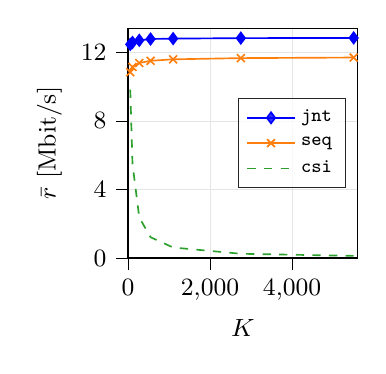
\begin{tikzpicture}

\definecolor{darkorange25512714}{RGB}{255,127,14}
\definecolor{forestgreen4416044}{RGB}{44,160,44}
\definecolor{lavender233}{RGB}{233,233,233}
\definecolor{lightgray204}{RGB}{204,204,204}
\definecolor{steelblue31119180}{RGB}{31,119,180}

\begin{axis}[
height=4.5cm,
width=4.5cm,
legend cell align={left},
legend style={
  at={(0.95,0.5)},
  anchor=east,
},
tick align=outside,
tick pos=left,
xlabel={\(\displaystyle K\)},
xmajorgrids,
xmin=0, xmax=5600,
ylabel={$\bar{r}$ [Mbit/s]},
ymajorgrids,
ymin=0, ymax=13.4,
ytick={0,4,8,12,16},
yticklabels={
  \(\displaystyle {0}\),  
  \(\displaystyle {4}\),  
  \(\displaystyle {8}\),  
  \(\displaystyle {12}\),  
  \(\displaystyle {16}\)
}
]
% kappa -9
\addplot [semithick, blue, mark=diamond*, mark size=2, mark options={solid}]
table {%
55 12.4591638807284
110 12.5701536588773
275 12.6935160461787
550 12.7707188464804
1100 12.7940235664421
2750 12.8223251573294
5500 12.8347220016408
};
\addlegendentry{\texttt{jnt}}
\addplot [semithick, darkorange25512714, mark=x, mark size=2, mark options={solid}]
table {%
55 10.833729732105
110 11.1402765877564
275 11.3707952474629
550 11.5018852764772
1100 11.5867252518525
2750 11.6571920560123
5500 11.6912288290793
};
\addlegendentry{\texttt{seq}}
\addplot [semithick, forestgreen4416044, dashed]
table {%
55 9.82513393032722
110 5.47815589153312
275 2.36519895283018
550 1.21233467996489
1100 0.613706141716637
2750 0.248056895571638
5500 0.124500295417333
};
\addlegendentry{\texttt{csi}}

% \draw[rounded corners=4.5pt, draw=black] (axis cs:900, 12.8) rectangle (axis cs:1300, 15.3);
% \node[align=left] at (axis cs:1000, 15.8) {$\kappa = 0$ dB};


\end{axis}
\end{tikzpicture}

    \vspace{-0.6cm}
    \caption{$\kappa = -9$ dB}
    \end{subfigure}
    ~
    \begin{subfigure}[t]{.45\columnwidth}
    % This file was created with tikzplotlib v0.10.1.
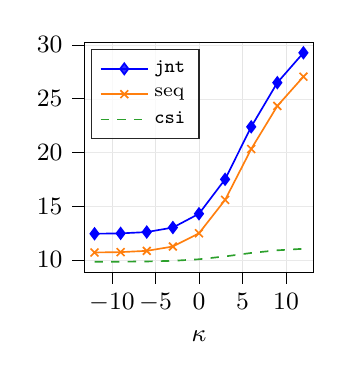
\begin{tikzpicture}

\definecolor{darkorange25512714}{RGB}{255,127,14}
\definecolor{forestgreen4416044}{RGB}{44,160,44}
\definecolor{lavender233}{RGB}{233,233,233}
\definecolor{lightgray204}{RGB}{204,204,204}
\definecolor{steelblue31119180}{RGB}{31,119,180}

\begin{axis}[
width=4.5cm,
height=4.5cm,
legend cell align={left},
legend style={
  at={(0.03,0.97)},
  anchor=north west,
},
tick align=outside,
tick pos=left,
xlabel={\(\displaystyle \kappa\)},
xmajorgrids,
xmin=-13.2, xmax=13.2,
xtick style={color=black},
xtick={-15,-10,-5,0,5,10,15},
xticklabels={
  \(\displaystyle {\ensuremath{-}15}\),
  \(\displaystyle {\ensuremath{-}10}\),
  \(\displaystyle {\ensuremath{-}5}\),
  \(\displaystyle {0}\),
  \(\displaystyle {5}\),
  \(\displaystyle {10}\),
  \(\displaystyle {15}\)
},
y grid style={lavender233},
% ylabel={throughput [Mbit/s]},
ymajorgrids,
ymin=8.85151856515297, ymax=30.2401732554369,
% ytick={7.5,10,12.5,15,17.5,20,22.5,25,27.5,30,32.5},
% yticklabels={
%   \(\displaystyle {7.5}\),
%   \(\displaystyle {10.0}\),
%   \(\displaystyle {12.5}\),
%   \(\displaystyle {15.0}\),
%   \(\displaystyle {17.5}\),
%   \(\displaystyle {20.0}\),
%   \(\displaystyle {22.5}\),
%   \(\displaystyle {25.0}\),
%   \(\displaystyle {27.5}\),
%   \(\displaystyle {30.0}\),
%   \(\displaystyle {32.5}\)
% }
]
\addplot [semithick, blue, mark=diamond*, mark size=2, mark options={solid}]
table {%
-12 12.4253106471137
-9 12.4591638807284
-6 12.582139971413
-3 13.0008775582797
0 14.2841671286686
3 17.4916631555555
6 22.3769478059178
9 26.486869304421
12 29.2679616786058
};
\addlegendentry{\texttt{jnt}}
\addplot [semithick, darkorange25512714, mark=x, mark size=2, mark options={solid}]
table {%
-12 10.6815308282906
-9 10.7148854519774
-6 10.833729732105
-3 11.2353867488805
0 12.4677671770795
3 15.5742720350395
6 20.3118302410626
9 24.3174212523339
12 27.0461267749496
};
\addlegendentry{seq}
\addplot [semithick, forestgreen4416044, dashed]
table {%
-12 9.82373014198406
-9 9.82513393032722
-6 9.84433921682666
-3 9.90570822272558
0 10.0498429168162
3 10.3158027189047
6 10.6369015559041
9 10.8840136701281
12 11.0271133097424
};
\addlegendentry{\texttt{csi}}
\end{axis}

\end{tikzpicture}

    \vspace{-0.15cm}
    \caption{$K = 55$}
    \end{subfigure}
    \caption{Max-rate performance.}
    \label{fig:max-rate}
\end{figure}

Fig.~\ref{fig:max-rate} shows the performance obtained by the max-rate allocation schemes. Fig.~\ref{fig:max-rate}(a) presents the throughput as a function of the number of users $K$ when $\kappa = -9$ dB, while Fig.~\ref{fig:max-rate}(b) as a function of the Rician $\kappa$ factor when $K = 55$. Both localization-based paradigms outperform the CSI-based scheme. In particular, when the system is in an overloaded state, i.e., $K > F S$, the \gls{CE} overhead increases in a prohibitive manner. Interestingly, even with a low number of users, the localization-based schemes achieve superior performance for every value of $\kappa$ under test.


\begin{figure}[thb]
    \centering
    \begin{subfigure}[t]{.45\columnwidth}
    \centering
    % This file was created with tikzplotlib v0.10.1.
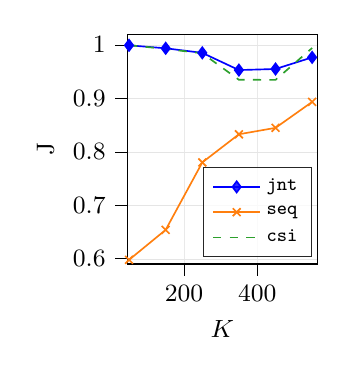
\begin{tikzpicture}

\definecolor{darkorange25512714}{RGB}{255,127,14}
\definecolor{forestgreen4416044}{RGB}{44,160,44}
\definecolor{lavender233}{RGB}{233,233,233}
\definecolor{lightgray204}{RGB}{204,204,204}
\definecolor{steelblue31119180}{RGB}{31,119,180}

\begin{axis}[
width=4cm,
height=4.5cm,
legend cell align={left},
legend style={    
  at={(0.97,0.03)},
  anchor=south east,  
},
tick align=outside,
tick pos=left,
x grid style={lavender233},
xlabel={\(\displaystyle K\)},
xmajorgrids,
xmin=45, xmax=565,
% xtick={0,100,200,300,400,500,600},
% xticklabels={
%   \(\displaystyle {0}\),
%   \(\displaystyle {100}\),
%   \(\displaystyle {200}\),
%   \(\displaystyle {300}\),
%   \(\displaystyle {400}\),
%   \(\displaystyle {500}\),
%   \(\displaystyle {600}\)
% },
ylabel={J},
ymajorgrids,
ymin=0.59, ymax=1.02,
% ytick={0.55,0.6,0.65,0.7,0.75,0.8,0.85,0.9,0.95,1,1.05},
% yticklabels={
%   \(\displaystyle {0.55}\),
%   \(\displaystyle {0.60}\),
%   \(\displaystyle {0.65}\),
%   \(\displaystyle {0.70}\),
%   \(\displaystyle {0.75}\),
%   \(\displaystyle {0.80}\),
%   \(\displaystyle {0.85}\),
%   \(\displaystyle {0.90}\),
%   \(\displaystyle {0.95}\),
%   \(\displaystyle {1.00}\),
%   \(\displaystyle {1.05}\)
% }
]
\addplot [semithick, blue, mark=diamond*, mark size=2, mark options={solid}]
table {%
50 0.999243175182723
150 0.993687367218431
250 0.985143131611637
350 0.952952148422242
450 0.954962947982503
550 0.976677116758078
};
\addlegendentry{\texttt{jnt}}
\addplot [semithick, darkorange25512714, mark=x, mark size=2, mark options={solid}]
table {%
50 0.597780849098348
150 0.653956906662436
250 0.780085171473543
350 0.832804255726962
450 0.844830327950017
550 0.893363834964714
};
\addlegendentry{\texttt{seq}}
\addplot [semithick, forestgreen4416044, dashed]
table {%
50 0.99954520334938
150 0.992487928448371
250 0.984377203977808
350 0.934768614966926
450 0.934606977131258
550 0.994244305910316
};
\addlegendentry{\texttt{csi}}
\end{axis}

\end{tikzpicture}

    \vspace{-0.2cm}
    \caption{$\kappa = -9$ dB}
    \end{subfigure}
    ~
    \begin{subfigure}[t]{.45\columnwidth}
    % This file was created with tikzplotlib v0.10.1.
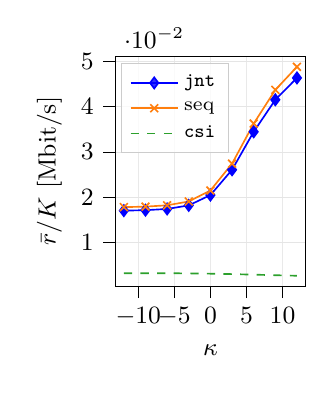
\begin{tikzpicture}

\definecolor{darkorange25512714}{RGB}{255,127,14}
\definecolor{forestgreen4416044}{RGB}{44,160,44}
\definecolor{lavender233}{RGB}{233,233,233}
\definecolor{lightgray204}{RGB}{204,204,204}
\definecolor{steelblue31119180}{RGB}{31,119,180}

\begin{axis}[
width=4cm,
height=4.5cm,
legend cell align={left},
legend style={
  fill opacity=0.8,
  draw opacity=1,
  text opacity=1,
  at={(0.03,0.97)},
  anchor=north west,
  draw=lightgray204
},
tick align=outside,
tick pos=left,
x grid style={lavender233},
xlabel={\(\displaystyle \kappa\)},
xmajorgrids,
xmin=-13.2, xmax=13.2,
xtick style={color=black},
xtick={-15,-10,-5,0,5,10,15},
xticklabels={
  \(\displaystyle {\ensuremath{-}15}\),
  \(\displaystyle {\ensuremath{-}10}\),
  \(\displaystyle {\ensuremath{-}5}\),
  \(\displaystyle {0}\),
  \(\displaystyle {5}\),
  \(\displaystyle {10}\),
  \(\displaystyle {15}\)
},
ylabel={$\bar{r} / K$ [Mbit/s]},
ymajorgrids,
ymin=0.000300957579279767, ymax=0.0510836953745609,
ytick={0,0.01,0.02,0.03,0.04,0.05,0.06},
yticklabels={
  \(\displaystyle {0}\),
  \(\displaystyle {1}\),
  \(\displaystyle {2}\),
  \(\displaystyle {3}\),
  \(\displaystyle {4}\),
  \(\displaystyle {5}\),
  \(\displaystyle {6}\)
}
]
\addplot [semithick, blue, mark=diamond*, mark size=2, mark options={solid}]
table {%
-12 0.017000251648027
-9 0.0171010964796189
-6 0.0173696568632962
-3 0.0181577285664528
0 0.0204351952958227
3 0.0260241969197762
6 0.0344228229243866
9 0.0414986771419747
12 0.0463304628823666
};
\addlegendentry{\texttt{jnt}}
\addplot [semithick, darkorange25512714, mark=x, mark size=2, mark options={solid}]
table {%
-12 0.0177732295279551
-9 0.0178857928732386
-6 0.018178492661637
-3 0.0190242933067968
0 0.0214514239847763
3 0.0273758130754146
6 0.0362343673946174
9 0.0436866553580576
12 0.048775389111139
};
\addlegendentry{seq}
\addplot [semithick, forestgreen4416044, dashed]
table {%
-12 0.00317995938227601
-9 0.00317558316780354
-6 0.00316296850567068
-3 0.00313080517468929
0 0.00306783547733286
3 0.00297246980402384
6 0.00285335995232013
9 0.00272741471281966
12 0.00260926384270163
};
\addlegendentry{\texttt{csi}}
\end{axis}

\end{tikzpicture}

    \vspace{-0.2cm}
    \caption{$K = 550$}
    \end{subfigure}
    \caption{Min-max performance.}
    \label{fig:min-max}
\end{figure}

Fig.~\ref{fig:min-max} shows the performance of the min-max allocation schemes. Fig.~\ref{fig:min-max}(a) presents the fairness as a function of the number of users $K$ when $\kappa = -9$ dB, while Fig.~\ref{fig:min-max}(b) the average throughput per user as a function of the Rician $\kappa$ factor when $K = 550$. In this case, the fairness performance of \texttt{jnt} and the \texttt{csi} are comparable, both outperforming \texttt{seq} for every $K$. Regarding the average throughput per user, the localization-based schemes outperform \texttt{csi}. In particular, \texttt{jnt} has a clear advantage to \texttt{csi} reaching similar fairness, but with an average rate more than doubled.


\section{Conclusions} \label{sec:conclusions}
This paper proposed an \gls{OFDM} framework for \gls{RIS}-aided communications that exploit localization information to perform a robust resource allocation in a multi-user scenario. The results presented show the effectiveness of the proposed approach w.r.t. \gls{CE}-based solutions.
While the proposed solution is promising, the impact of localization accuracy needs to be studied by investigating the trade-off of transmitting data and localization symbols.


%============================
% References
%============================
\bibliographystyle{IEEEtran}
\bibliography{loca.bib}
\end{document}
